% TODO: MOSTRAR FOTO DEL BOTON PINGPONG

\documentclass{article}
\usepackage[utf8]{inputenc}
\usepackage[spanish]{babel}
\usepackage{graphicx}	%Si se quiere compilar con las imagenes
% \usepackage[draft]{graphicx}	%Si NO se quiere compilar con las imagenes porque tarda mucho
\usepackage{graphics, float, fancyhdr, titling, caption, subcaption}
\usepackage{listings}
\usepackage[a4paper, total={6in, 9.5in}]{geometry}
\usepackage{fancyhdr}
\usepackage{hyperref}   %para que funcione addcontentsline debe ser la ultima que se cargue
\usepackage{amsmath}
%\setcounter{secnumdepth}{-2}       %Poner solo esto si no se quieren numero delante de las secciones y niveles inferiores.

\renewcommand{\footrulewidth}{0.4pt}
\title{

\includegraphics[width=1.75in]{imagenes/UGR-Logo.png} \\
\vspace*{1in}
\textbf{Memoria de la práctica 3} \\
Animación por Ordenador \\
\vspace*{0.5in}}
\author{Andrés Merlo Trujillo \\
andresmerlo@correo.ugr.es \\
77147239H \\ 
\vspace*{0.5in} \\
E.T.S. de Ingenierías Informática y de Telecomunicación \\
\textbf{Universidad de Granada}} \date{\today}

\hypersetup{
    colorlinks=true,
    linkcolor=black,
    citecolor=black
}

\renewcommand\maketitlehooka{\null\mbox{}\vfill}
\renewcommand\maketitlehookd{\vfill\null}

\begin{document}
\begin{titlingpage}
\maketitle
\end{titlingpage}

\tableofcontents

\newpage

\pagestyle{fancy}   %a partir de comienza el header (se salta el indice y portada)
\fancyhead[L]{Andrés Merlo Trujillo}
\fancyhead[R]{Animación por Ordenador}
%\section{Ejercicio 1}
%\begin{figure}[H]
%    \centering
%    \includegraphics[width=\textwidth]{imagenes/passwdfile.png}
%    \vspace{10pt}
%    \footnotesize{Fuente: https://...}
%\end{figure}

% \begin{figure}[H]
%     \centering 
% 	\begin{subfigure}[t]{0.48\textwidth}
% 	    \centering
% 	    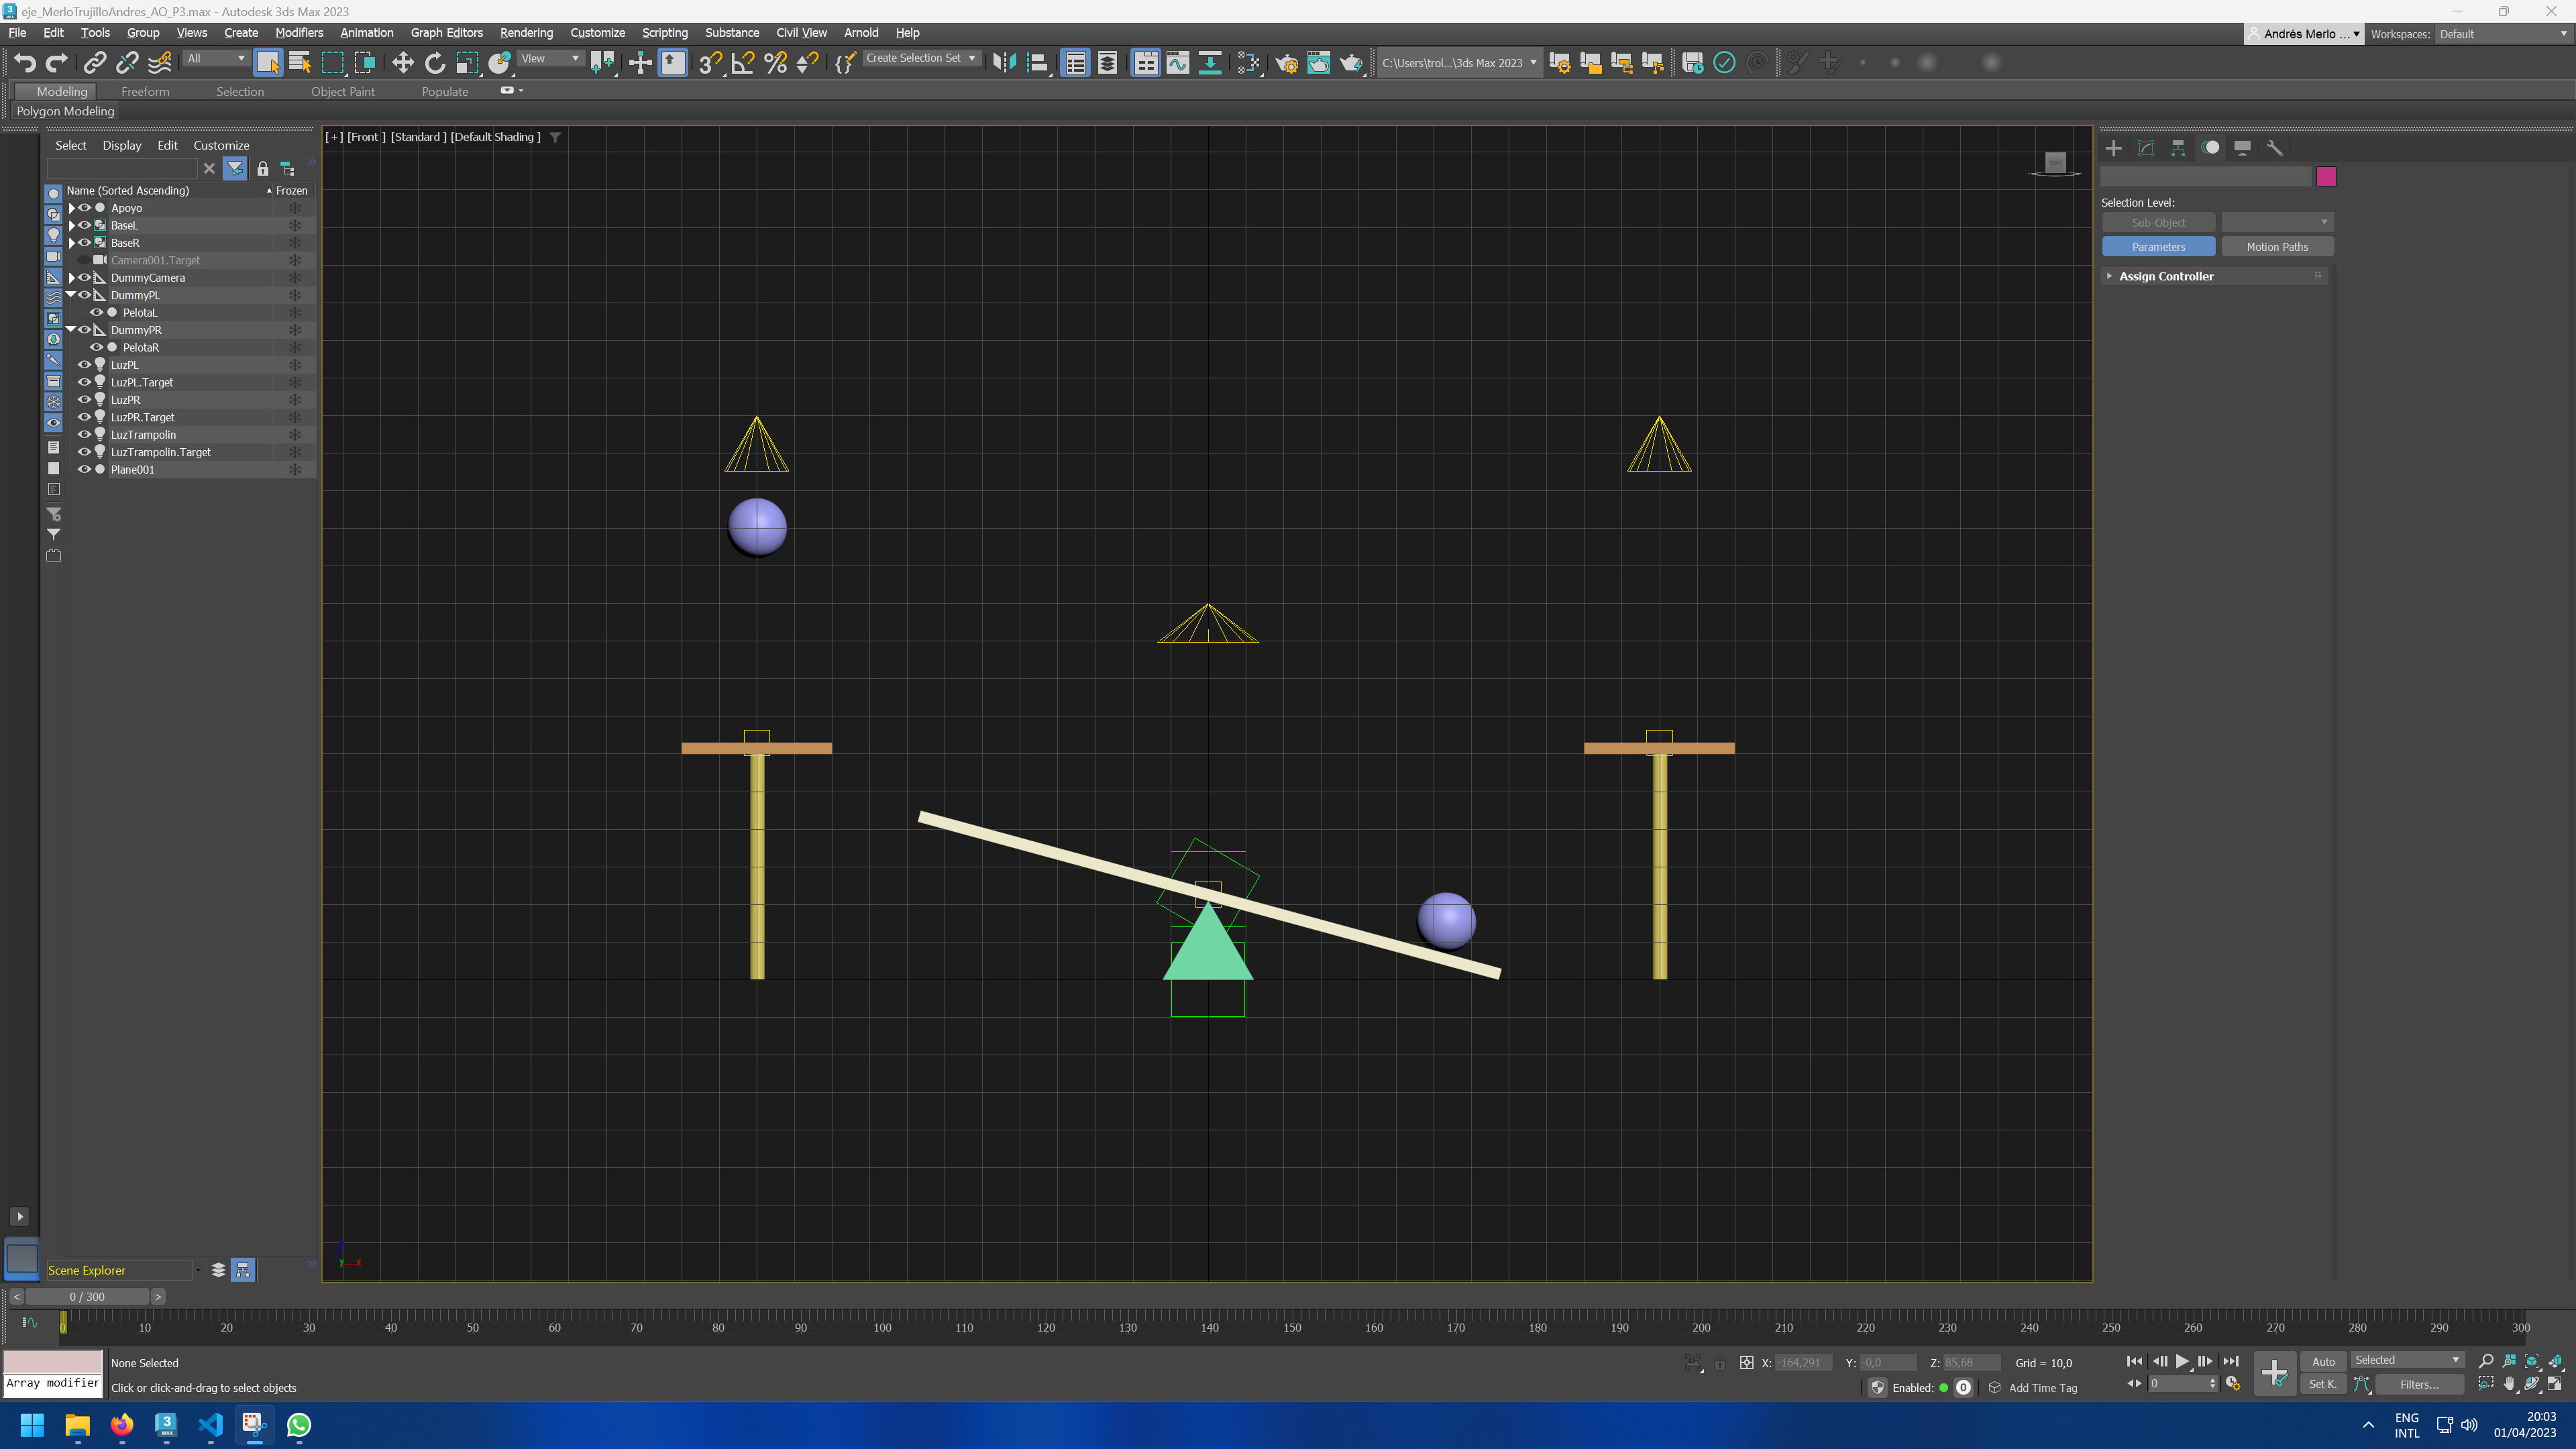
\includegraphics[width=\textwidth]{imagenes/Ejercicio 1/keyframes/0.png}
%         \caption{Pelotas en el instante 0.}
%     \end{subfigure}
%     \hfill
%     %\par\bigskip %si se desea dejar un margen entre la imagen de arriba y de abajo
% 	\begin{subfigure}[t]{0.48\textwidth}
% 	    \centering
% 	    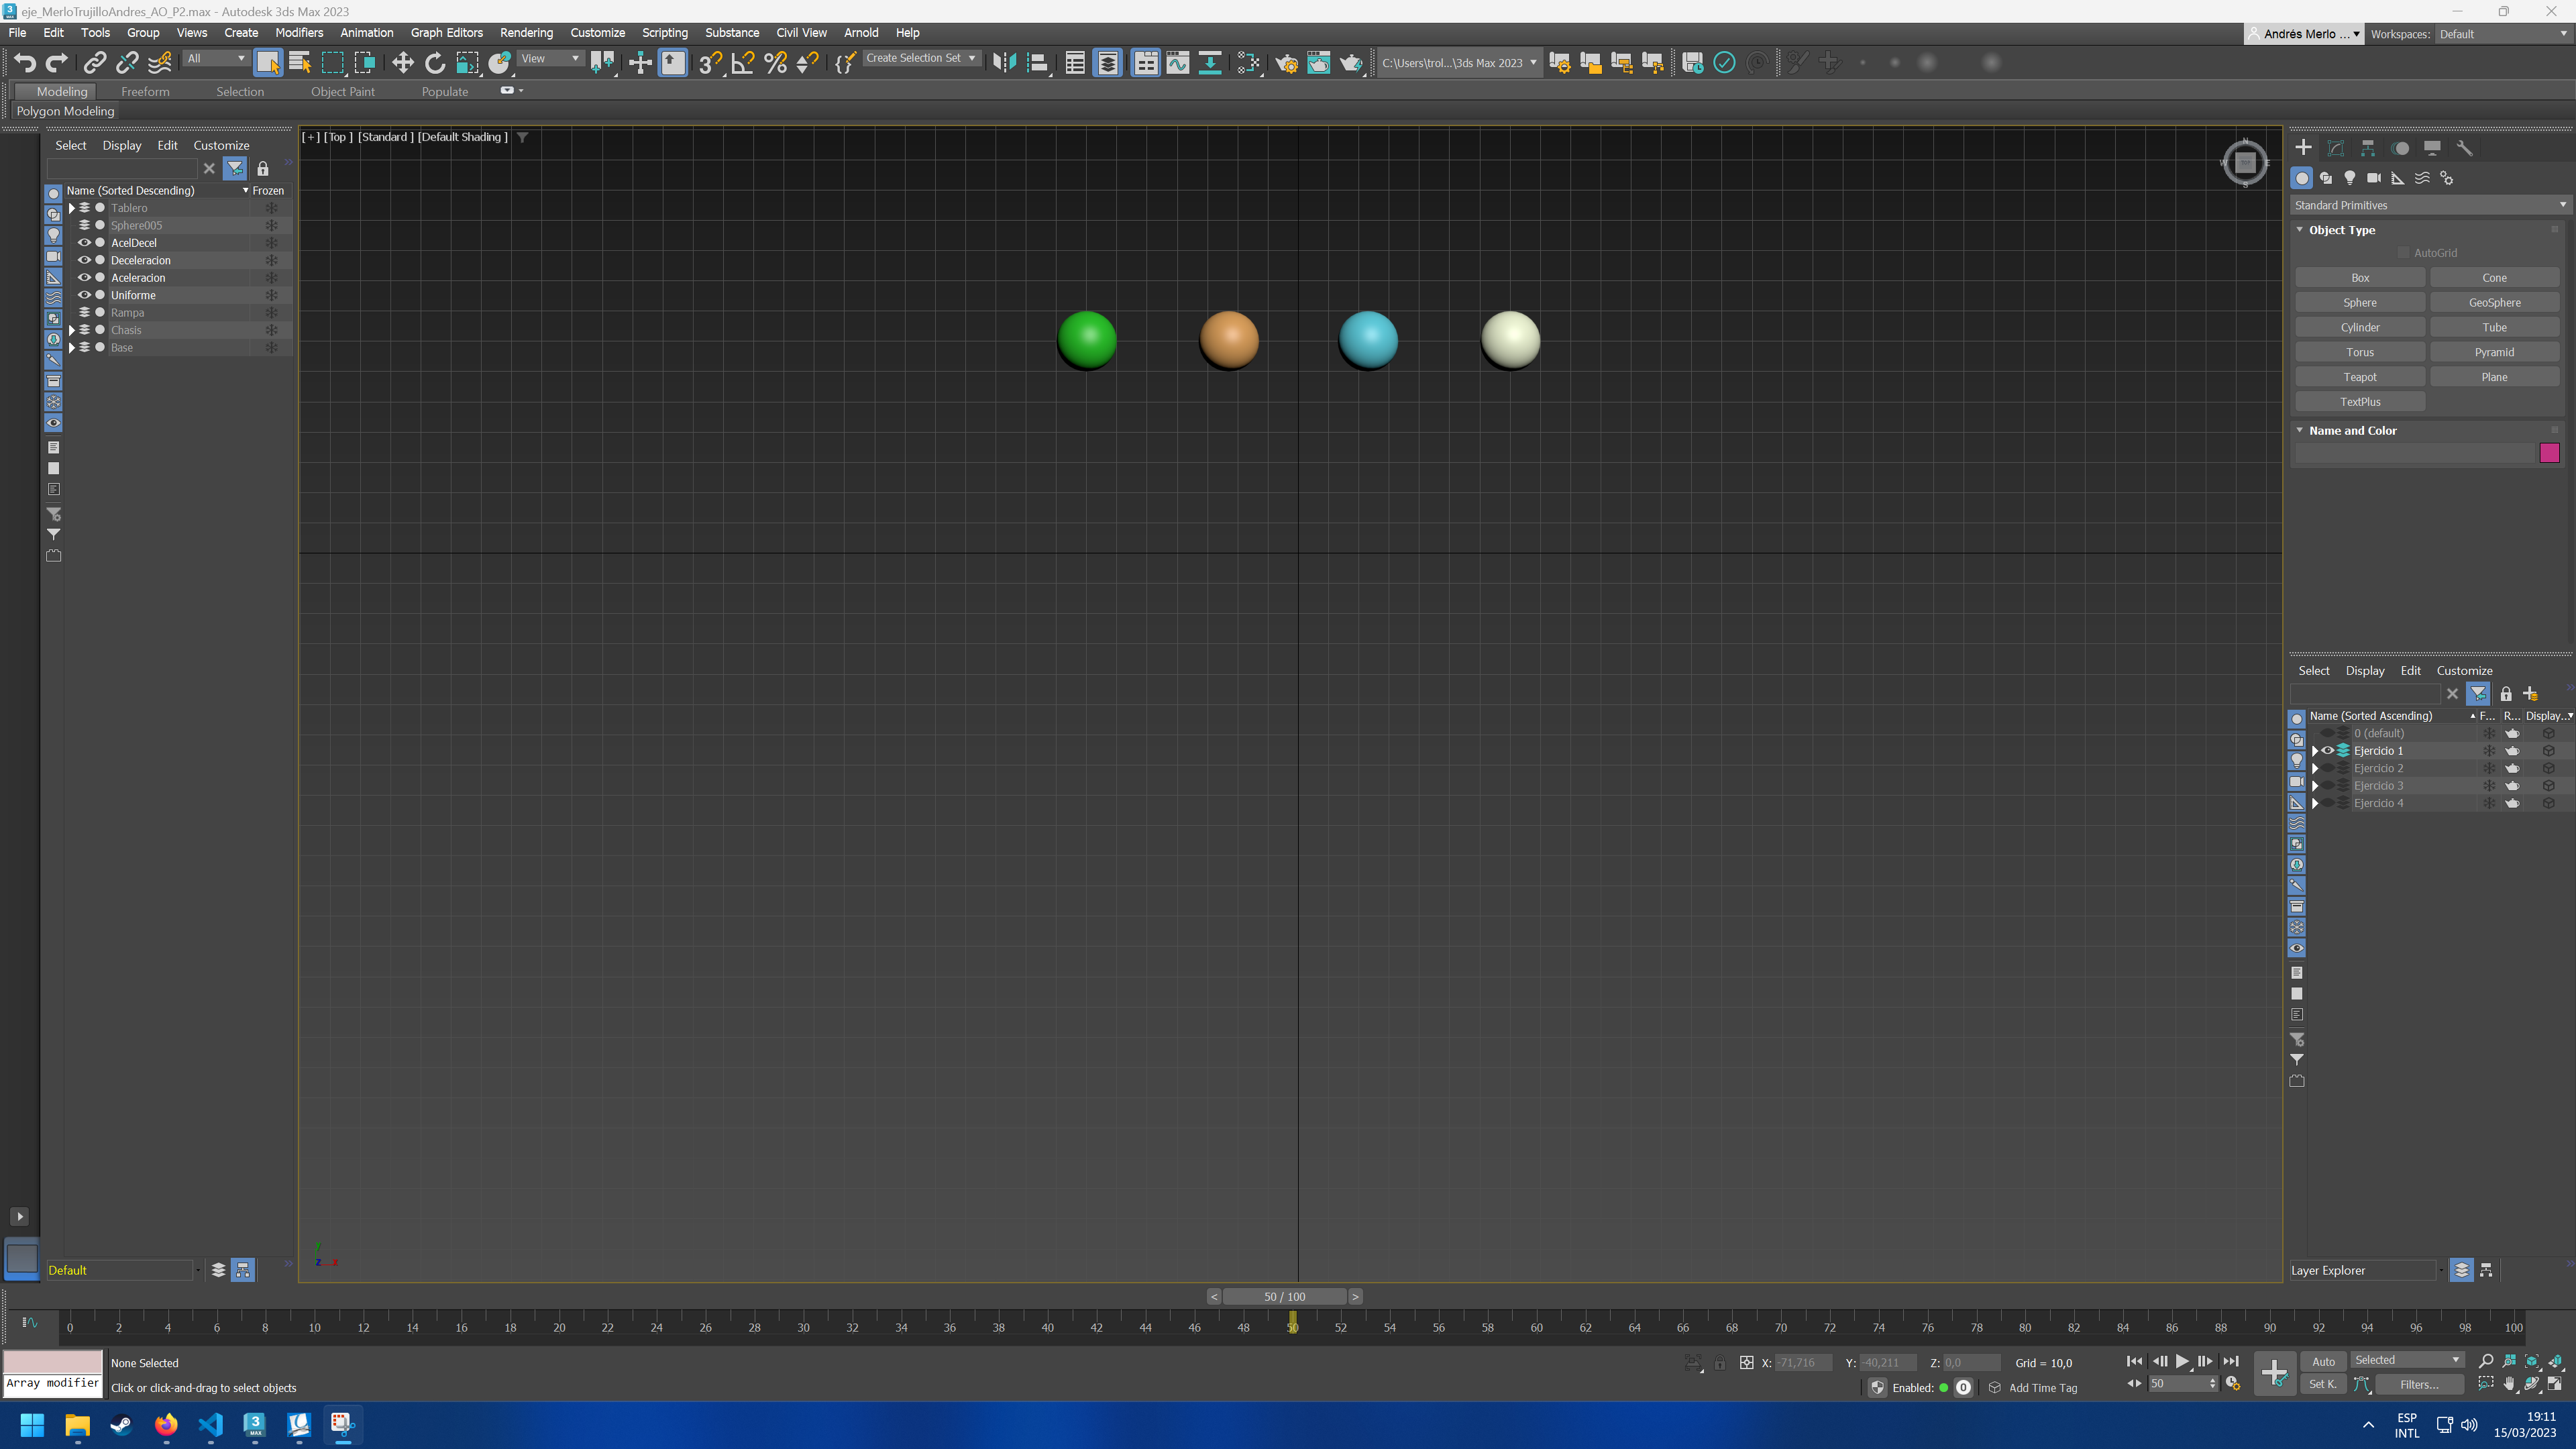
\includegraphics[width=\textwidth]{imagenes/Ejercicio 1/keyframes/50.png}
%         \caption{Pelotas en el instante 50.}
%     \end{subfigure}    
% \end{figure}


\section{Introducción}
En esta práctica se pide animar dos bolas. La primera bola botará varias veces y caerá a un trampolín, haciendo que la segunda bola, posada sobre dicho trampolín, sea lanzada y caiga sobre una plataforma. También se debe animar un conjunto de luces que iluminará la parte de la escena que está en movimiento actualmente y una cámara, que rotará alrededor de la escena.

\bigskip

Todo lo mencionado anteriormente se debe repetir de forma invertida, de manera que cuando acabe la animación vuelva a realizarse, pero al revés, comenzando por el final y acabando por el principio.

\bigskip

En esta memoria, voy a dividir cada una de las partes que he realizado en secciones, las cuales se presentarán a continuación.

\section{Duración de la escena}

% rescribir
En la práctica se pedía que la animación durara 5 segundos, seguidos de otros 5 segundos para la animación inversa. 

\bigskip

En mi caso, he utilizado 30 fotogramas por segundo, que es el valor por defecto en 3ds Max. Por lo tanto, los cálculos necesarios para obtener el número de fotogramas son los siguientes:

\bigskip

$30 \text{ fps} \times 2 \times 5 \text{ segundos} = 300 \text{ fotogramas} $

\bigskip

Cabe destacar que este valor hay que ponerlo en la casilla \textit{Length}, ya que es la que indica la longitud de tiempo que va a tener la escena. Además, la animación debe acabar en el instante 150, para dar paso a la animación inversa y que esta se complete antes de comenzar de nuevo por el principio.

\bigskip

La ventana con la configuración es la siguiente:

\begin{figure}[H]
   \centering
   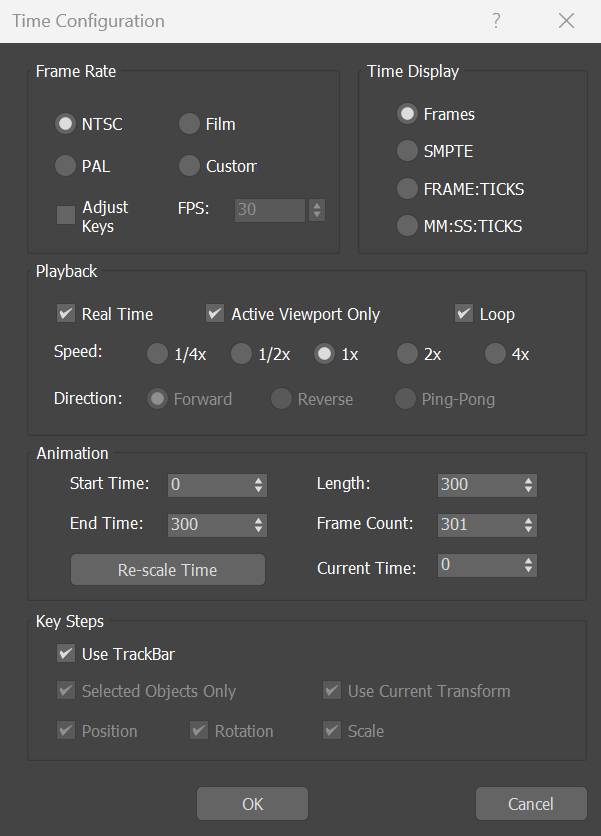
\includegraphics[width=0.5\textwidth]{imagenes/misc/duracion.png}
   \caption{Configuración de la duración de la escena.}
\end{figure}

Como se puede observar, \textit{Frame Count} indica un valor de 301, pero, según la documentación (\href{https://help.autodesk.com/view/3DSMAX/2022/ENU/?guid=GUID-9473CAF3-AF73-4127-A98C-58ACEF01ACAC}{Enlace}), siempre será la longitud más 1, por lo que realmente no hay que fijarse en este valor. Otra forma de comprobar que es correcto es cambiar el \textit{Time Display} a ``MM:SS:TICKS'' y mirando las casillas \textit{End Time} y \textit{Length}, que indican 10 segundos.
\section{Composición de los objetos}

Los distintos objetos de la escena se han construido de la siguiente forma:

\begin{itemize}
    \item \textbf{Trampolín: }He utilizado un cubo achatado y estirado para hacer la tabla y para el punto de apoyo he usado un cilindro con una base de 3 aristas, haciendo que sea un triángulo.
    
    Además, he modificado el pivote del tablero para que se encuentre justo en la unión del punto de apoyo con la tabla, con el objetivo de que gire de manera realista.

    Cabe destacar que he realizado una jerarquía en la que el punto de apoyo es el padre.

    \begin{figure}[H]
      \centering
      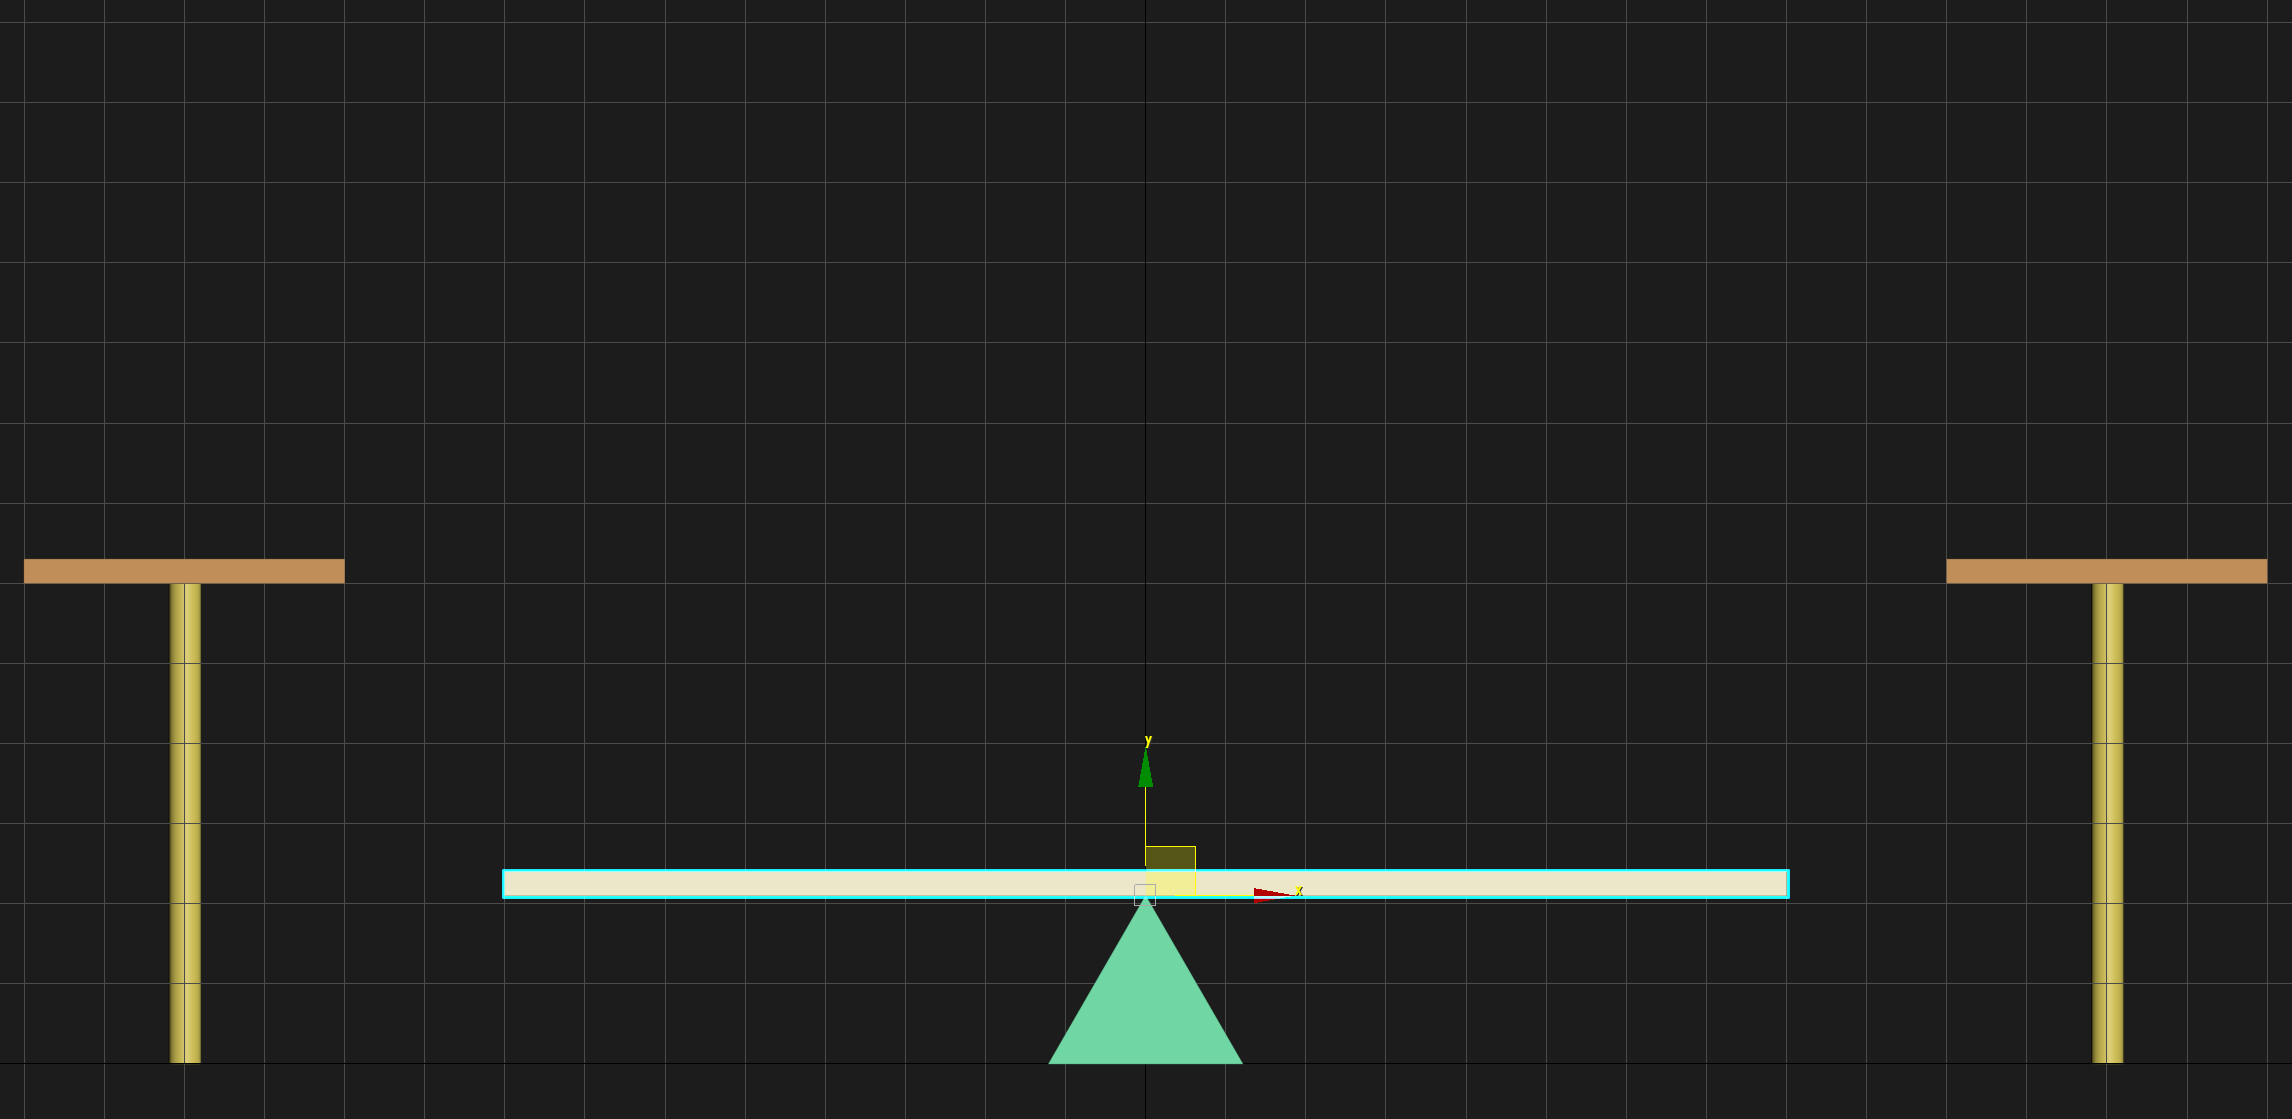
\includegraphics[width=0.7\textwidth]{imagenes/misc/PivotTrampolin.png}
      \caption{Pivote de la plataforma del trampolín.}
   \end{figure}

    \item \textbf{Bases: }Para las bases he utilizado un cubo achatado y un cilindro para el soporte, uniendo ambos en un grupo.
\end{itemize}

\newpage

\section{Animación de la escena}

La animación la he realizado algo distinta a la que se pedía en el guion, ya que le comenté al profesor que el resultado final era muy lento y me dijo que podía añadir algunos rebotes antes de comenzar la animación pedida. Para dar simetría, he animado dos rebotes al principio de la animación y al final y en ambas pelotas, para que la repetición inversa sea igual. 

\bigskip

Además, se pide hacer que los últimos 5 segundos realice la misma animación, pero al revés. Esto se realiza usando la forma ping-pong, accesible desde la ventana para el editor de curvas.

\begin{figure}[H]
   \centering
   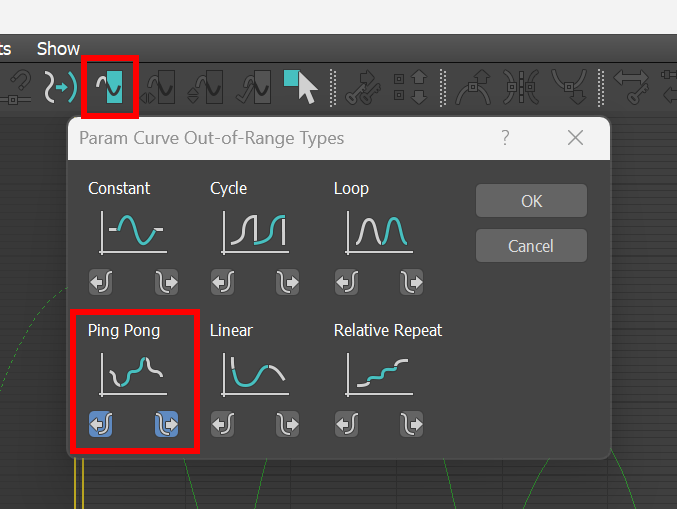
\includegraphics[width=0.5\textwidth]{imagenes/misc/ping-pong.png}
   \caption{Pasos necesarios para seleccionar el tipo ping-pong.}
\end{figure}

Esta forma obliga a repetir \textit{keyframes} en los instantes 0 y 150; es decir, no va a haber cambio con el \textit{keyframe} siguiente o anterior. Esto es necesario porque hay animaciones que no duran lo mismo, como el balancín, que su animación es más corta y si no se hiciera daría como resultado un giro prematuro, haciendo que la animación no sea correcta en los últimos 5 segundos.

\bigskip

% rescribir
Para animar el movimiento de las pelotas, he usado un objeto \textit{Dummy} con centro en la superficie donde tocan las pelotas el balancín y centrado en el eje X. Este objeto será padre de las pelotas en la jerarquía.

\bigskip

Asimismo, para que la trayectoria que realicen no se vea afectada por la rotación del \textit{Dummy}, este se debe encontrar sin ninguna rotación en el momento en el que salen/entran al trampolín. Si no se siguiera esto, la trayectoria seguida en los saltos estaría rotada, de acuerdo al ángulo que tenga el \textit{Dummy} en ese momento.

\bigskip

% Ahora bien, como puede haber confusión sobre los distintos \textit{keyframes} para los objetos de la escena, voy a dividir cada objeto junto a su \textit{Dummy}, si lo tiene, en subsecciones:

Voy a dividir cada parte de la escena animada en subsecciones, que se encuentran a continuación.

\subsection{Pelota de la izquierda}

Los \textit{keyframes} para la pelota de la izquierda son:

\begin{itemize}
    \item \textbf{Instante 0: }La pelota se encuentra sobre su base, a cierta altura de la misma para realizar varios rebotes.
    \item \textbf{Instante 14: }La pelota se encuentra tocando la superficie de la base, debido a la caída de la pelota.
    \item \textbf{Instante 26: }La pelota se encuentra en el aire, con la misma altura que en el instante 0. No disminuyo la altura del rebote para que la animación ping-pong funcione de manera más o menos realista.
    \item \textbf{Instante 38: }La pelota se encuentra sobre la superficie de la base, esta vez lista para saltar al trampolín.
    \item \textbf{Instante 48: }La pelota se encuentra en su punto más alto del salto hacia el trampolín.
    \item \textbf{Instante 58: }La pelota ha caído y se encuentra sobre el trampolín.
    \item \textbf{Instante 150: }Exactamente igual que el instante anterior, para que la animación se pueda repetir correctamente.
\end{itemize}

\bigskip

Las curvas de animación para la pelota son:

\begin{figure}[H]
   \centering
   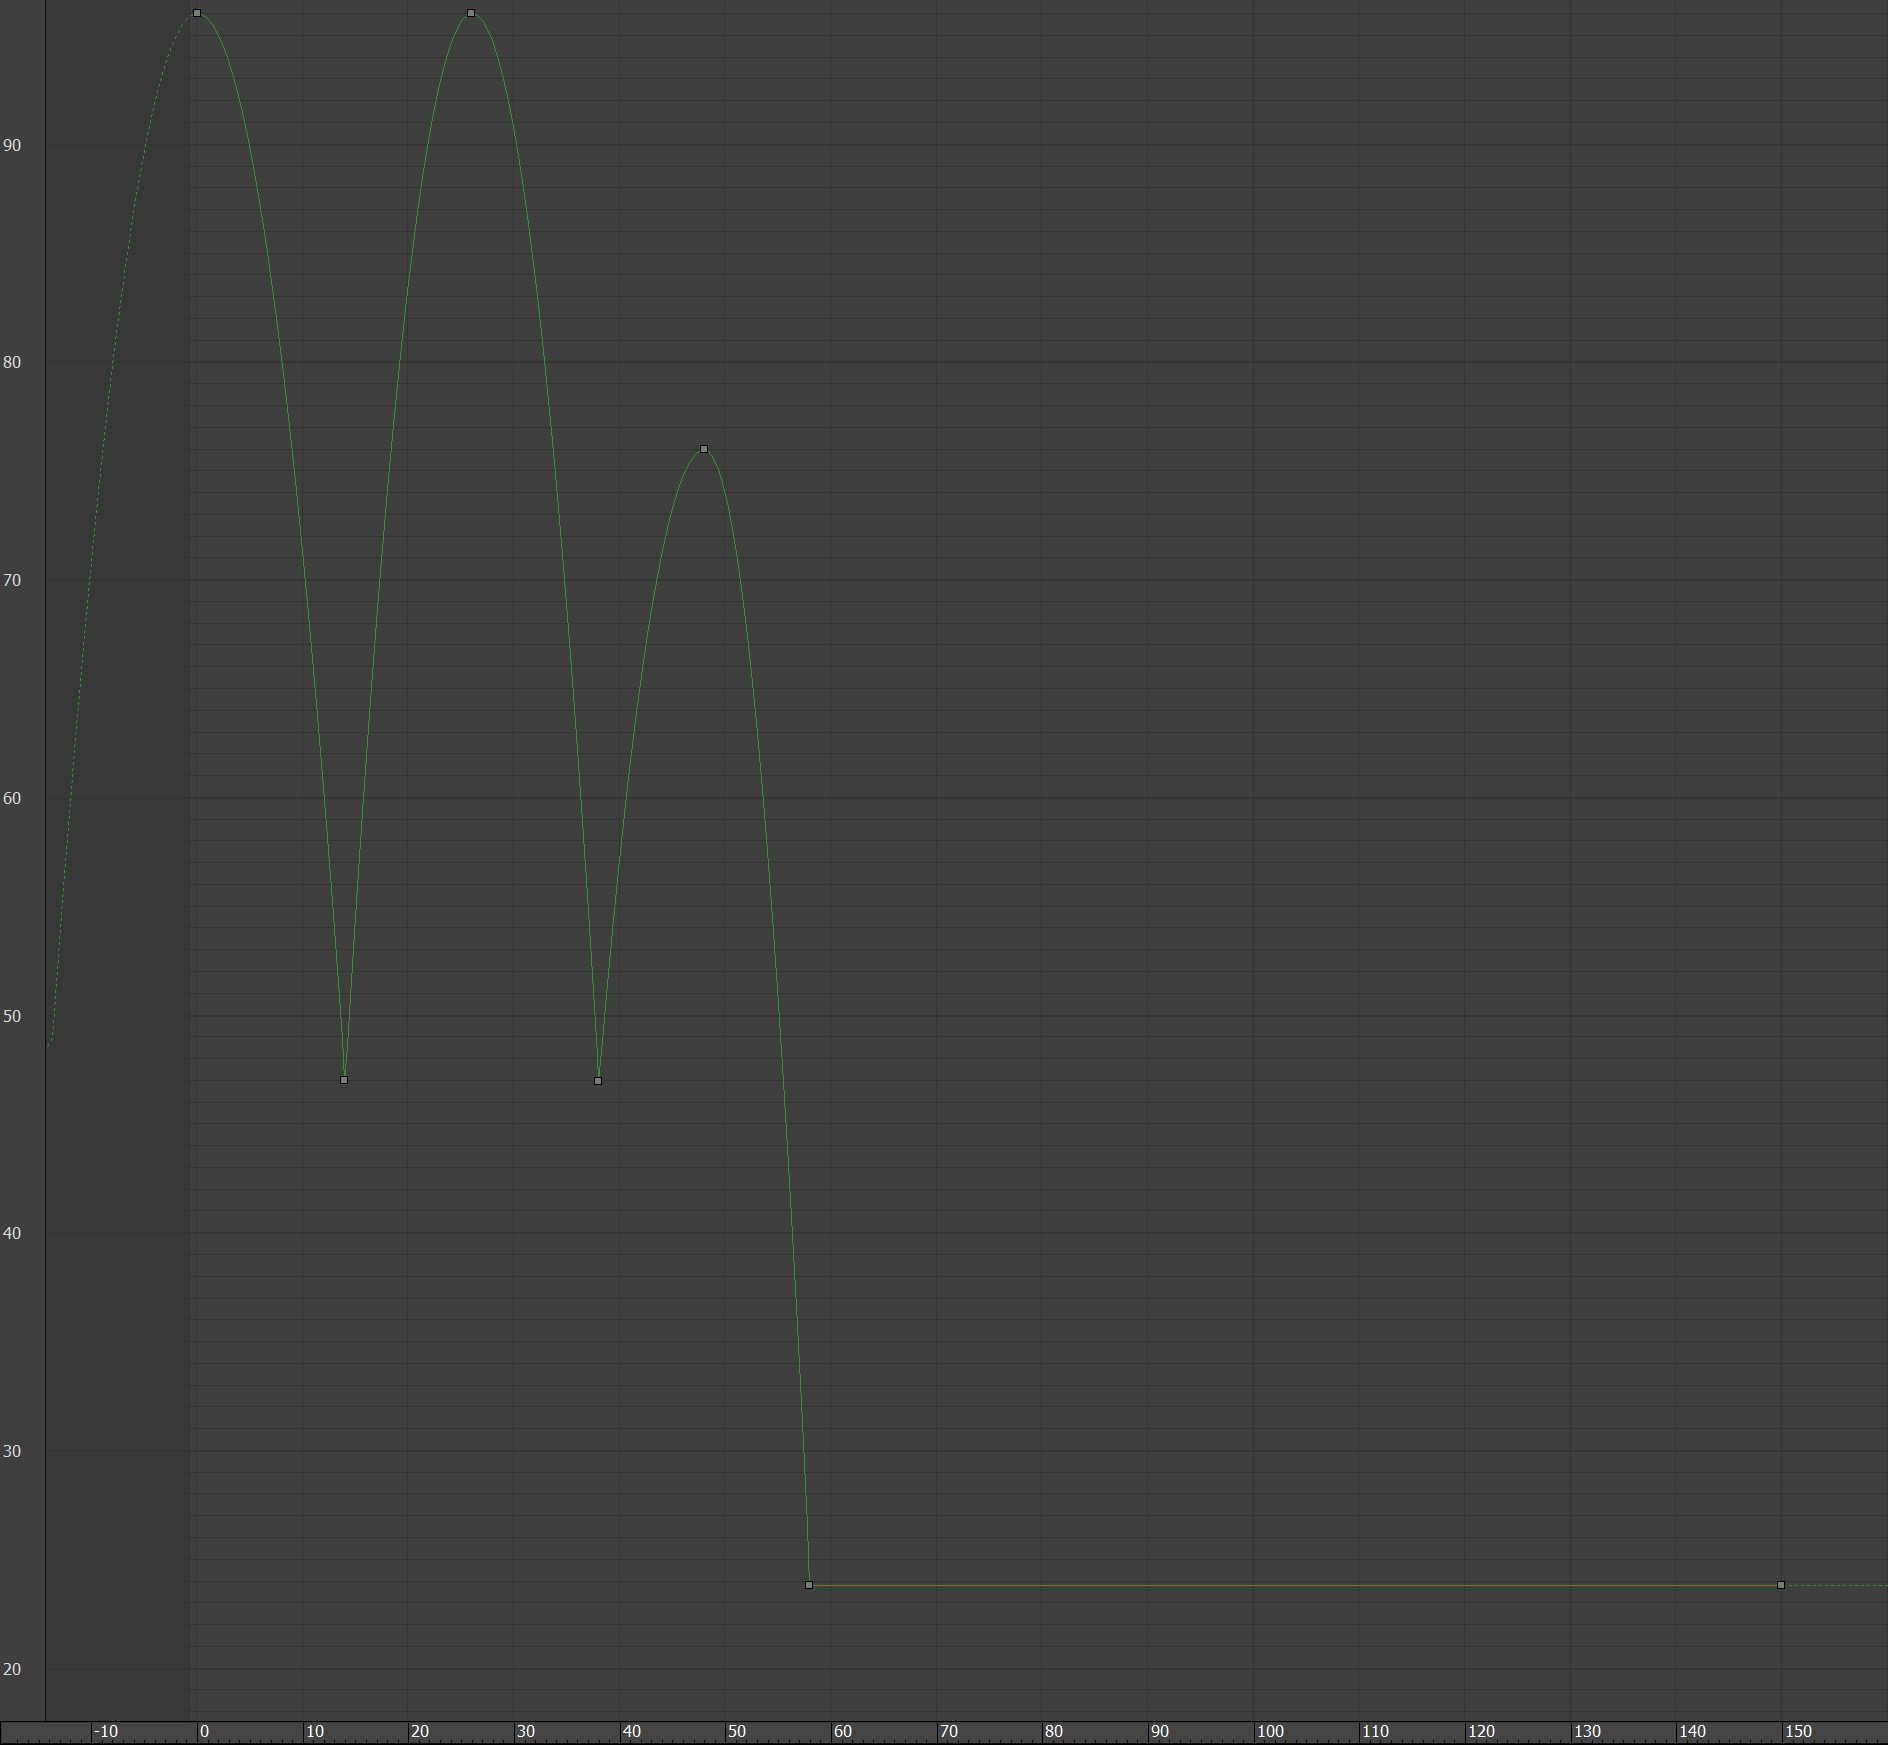
\includegraphics[width=0.6\textwidth]{imagenes/curvas/PL/pelota/green.png}
   \caption{Curva que representa la posición en el eje Y de la pelota con respecto el tiempo.}
\end{figure}

Esta curva representa la posición en el eje Y de la pelota con respecto el tiempo. Realmente se ve reflejado en un cambio en el eje Z en coordenadas del mundo, pero a causa de usar los \textit{dummies}, este eje cambia. Sabiendo esto, se puede ver como la curva realiza una forma parabólica, simulando los efectos que tiene la gravedad sobre la pelota para acelerarla en la bajada y desacelerarla en la subida. Finalmente se queda parada sobre el trampolín y dicho estado se extiende hasta el instante 150, para que la animación inversa funcione.

\begin{figure}[H]
   \centering
   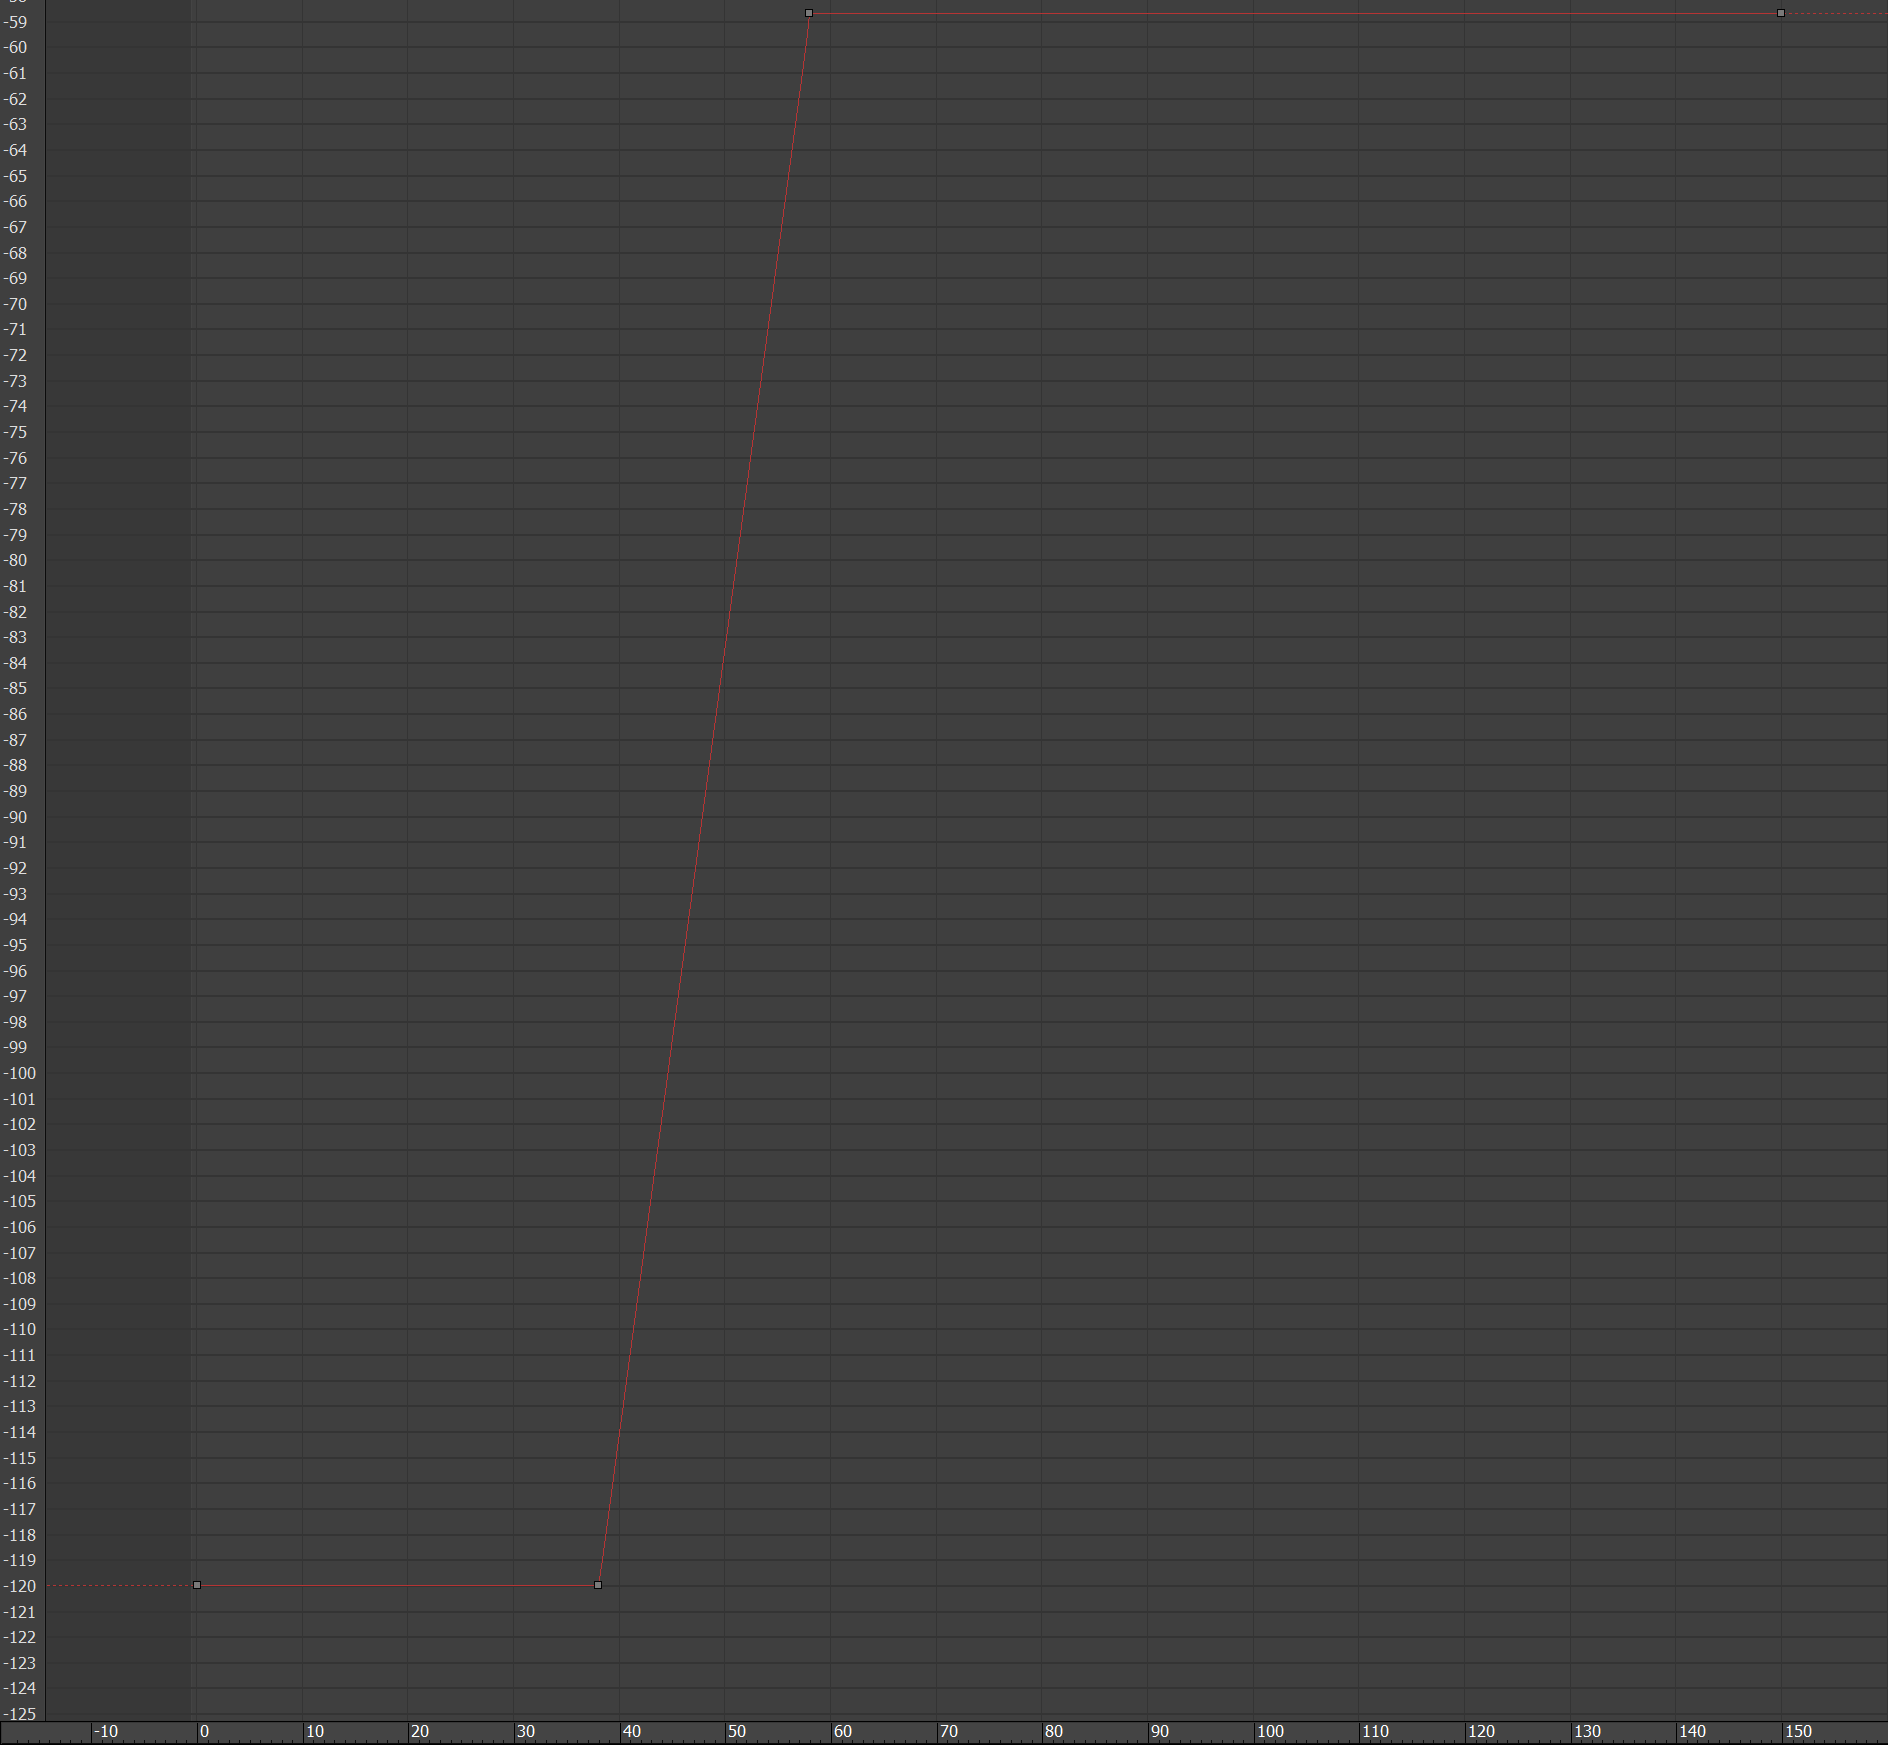
\includegraphics[width=0.6\textwidth]{imagenes/curvas/PL/pelota/red.png}
   \caption{Curva que representa la posición en el eje X con respecto el tiempo.}
\end{figure}

% rescribir
Esta curva representa la posición en el eje X con respecto el tiempo, solo desde la posición de la base hasta en el momento que toca por primera vez el trampolín, ya que las siguientes animaciones las realiza el \textit{Dummy} correspondiente. He elegido una función lineal porque es la que me ha parecido más realista de todas las opciones, dentro de lo que cabe. 

\bigskip

Los \textit{keyframes} para el \textit{Dummy} de la pelota de la izquierda son:

\begin{itemize}
    \item \textbf{Instante 0: }Se encuentra en su posición inicial, sin ninguna rotación para hacer que la trayectoria de la pelota sea correcta. Se hace para que la animación inversa funcione de manera correcta.
    \item \textbf{Instante 58: }Exactamente igual que el anterior \textit{keyframe}.
    \item \textbf{Instante 92: }El \textit{Dummy} se encuentra rotado hacia la izquierda, para animar el balanceo del balancín de manera correcta.
    \item \textbf{Instante 150: }Exactamente igual que el instante anterior, se hace para que la animación ping-pong comience al unísono con las demás.
\end{itemize}

\newpage

Las curva de animación para el \textit{Dummy} son:

\begin{figure}[H]
    \centering
    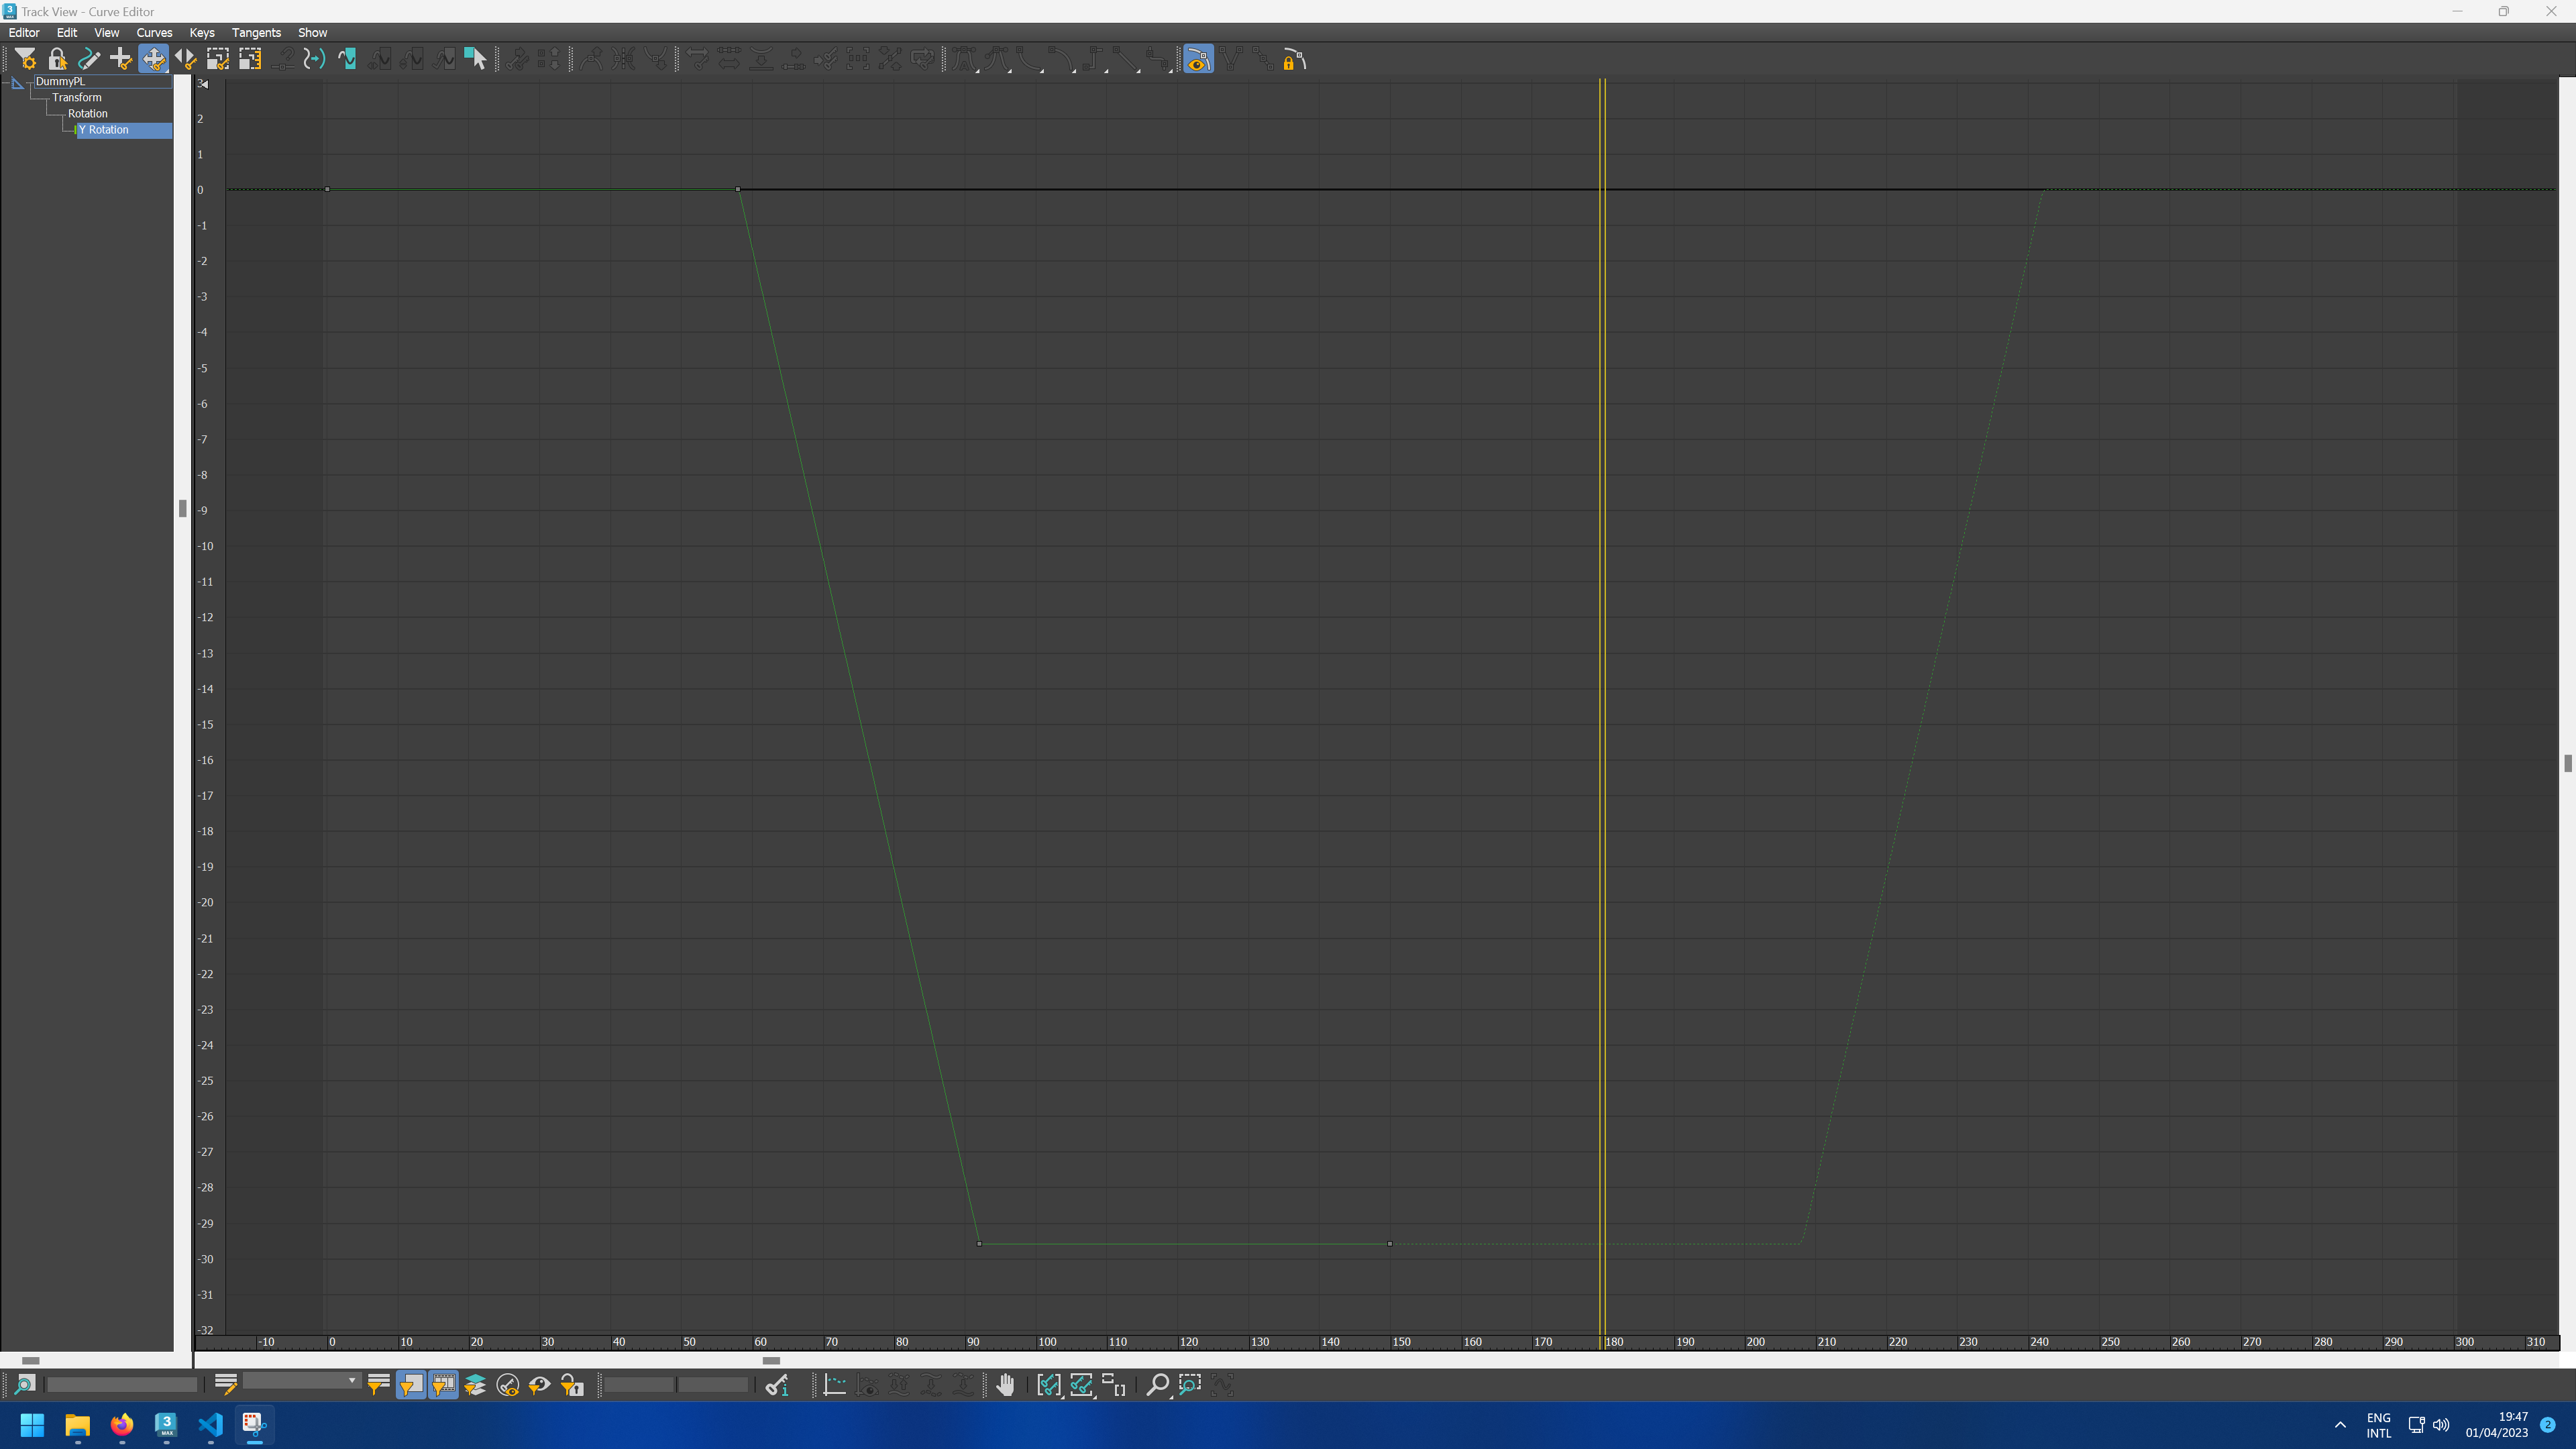
\includegraphics[width=0.6\textwidth]{imagenes/curvas/PL/dummy/green.png}
    \caption{Curva que representa la rotación en el eje Y con respecto el tiempo.}
 \end{figure}

 % rescribir, muy repetido trampolín y pelota
% Esta curva representa la rotación del \textit{dummy} con respecto al tiempo. La he animado de forma lineal porque, al seguir la animación del trampolín, esta debe seguirla también; es decir, como la energía potencial que tiene la pelota se le transfiere al trampolín, haciendo que el trampolín tenga la misma velocidad que la que tenía la pelota y no teniendo tiempo para acelerar.

Esta curva debe seguir la forma que la del trampolín, en este caso lineal, ya que debe girar al mismo tiempo ambos. La curva es lineal porque la pelota le transfiere la energía al trampolín, sin darle la oportunidad de acelerar y adquiriendo la velocidad que la bola tenía.

\bigskip

Todo esto que he dicho es aplicable al trampolín, por lo que la explicación correspondiente va a ser muy similar.

\bigskip

La pelota y su \textit{Dummy} se encuentran en la escena de la siguiente forma:

\begin{figure}[H]
   \centering
   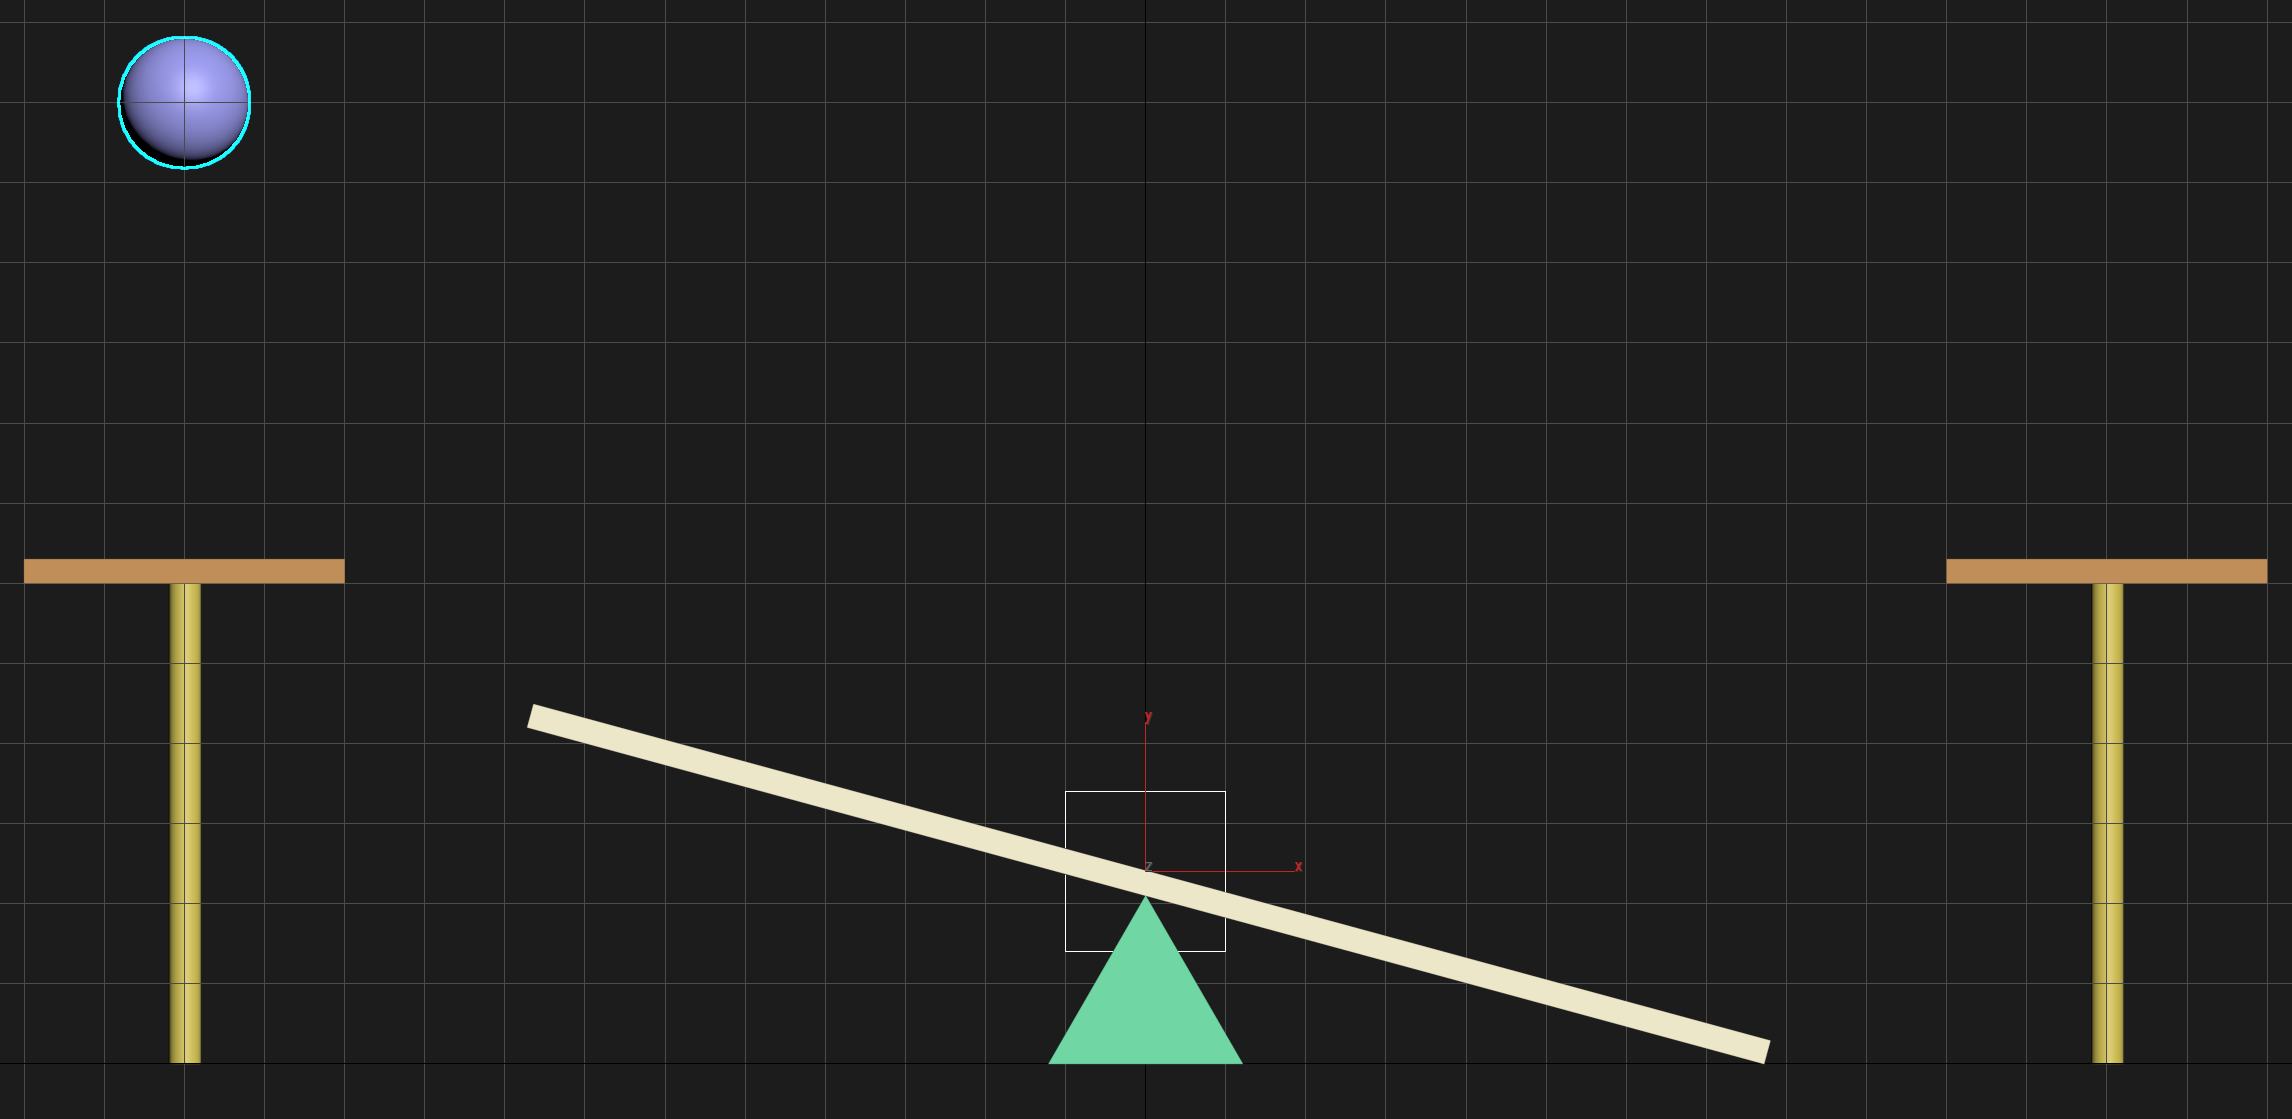
\includegraphics[width=0.7\textwidth]{imagenes/misc/PLDummy.png}
   \caption{Pelota izquierda junto a su \textit{Dummy}.}
\end{figure}


\newpage
\subsection{Pelota de la derecha}
Los \textit{keyframes} de la pelota de la derecha son:

\begin{itemize}
    \item \textbf{Instante 0: }La pelota se encuentra sobre la superficie del trampolín. Este instante solo es una extensión para que la animación ping-pong funcione correctamente y al mismo tiempo.
    \item \textbf{Instante 92: }Exactamente igual que el instante anterior.
    \item \textbf{Instante 102: }La pelota se encuentra sobre el punto más alto de la trayectoria hacia la base.
    \item \textbf{Instante 112: }La pelota ha acabado de realizar la trayectoria y se encuentra sobre la superficie de la base.
    \item \textbf{Instante 124: }La pelota se encuentra en el aire porque ha realizado un rebote.
    \item \textbf{Instante 136: }Ahora la pelota ha caído al suelo.
    \item \textbf{Instante 150: }Finalmente, la pelota da otro rebote y se encuentra en el aire de nuevo.
\end{itemize}

\bigskip

Las curvas de animación es:

\begin{figure}[H]
    \centering
    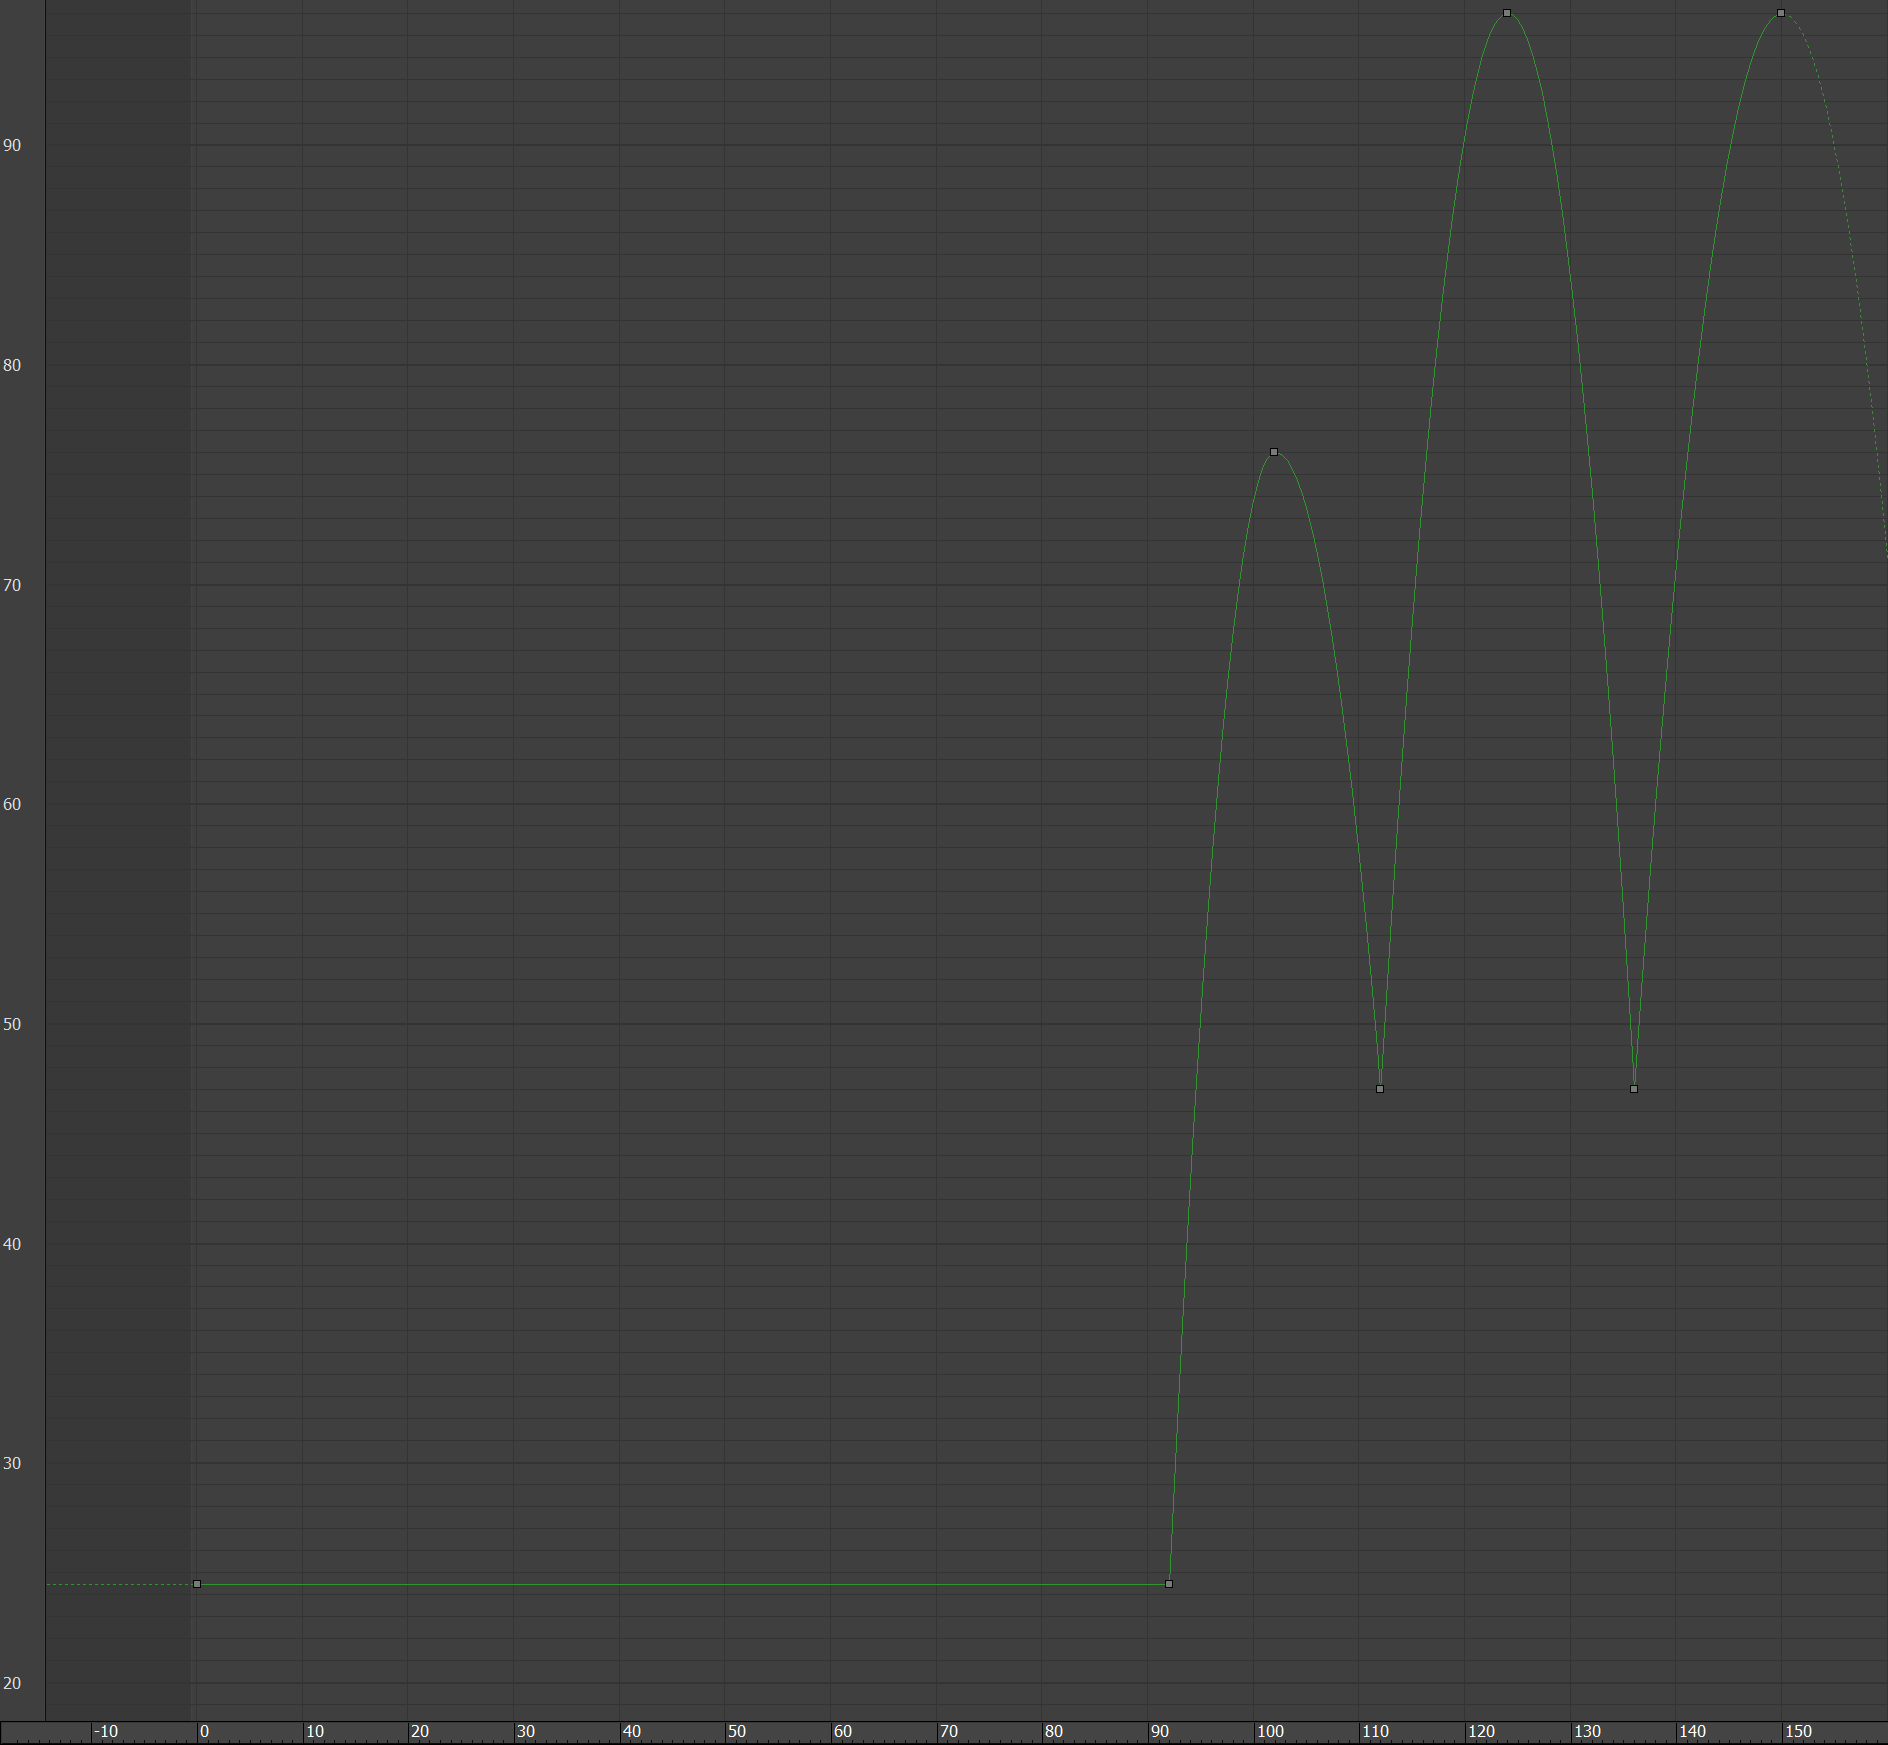
\includegraphics[width=0.6\textwidth]{imagenes/curvas/PR/pelota/green.png}
    \caption{Curva que representa la posición en el eje Y con respecto el tiempo.}
 \end{figure}

 Al igual que con la pelota de la izquierda, debido al \textit{Dummy} el eje Z pasa a ser el eje Y, pero en coordenadas del mundo sigue siendo el Z. Además, ocurre exactamente igual que en la pelota de la izquierda, se utilizan parábolas para simular los efectos de la gravedad sobre la pelota y que produzca un resultado natural, tanto en la trayectoria como en las subidas y caídas.

 \begin{figure}[H]
    \centering
    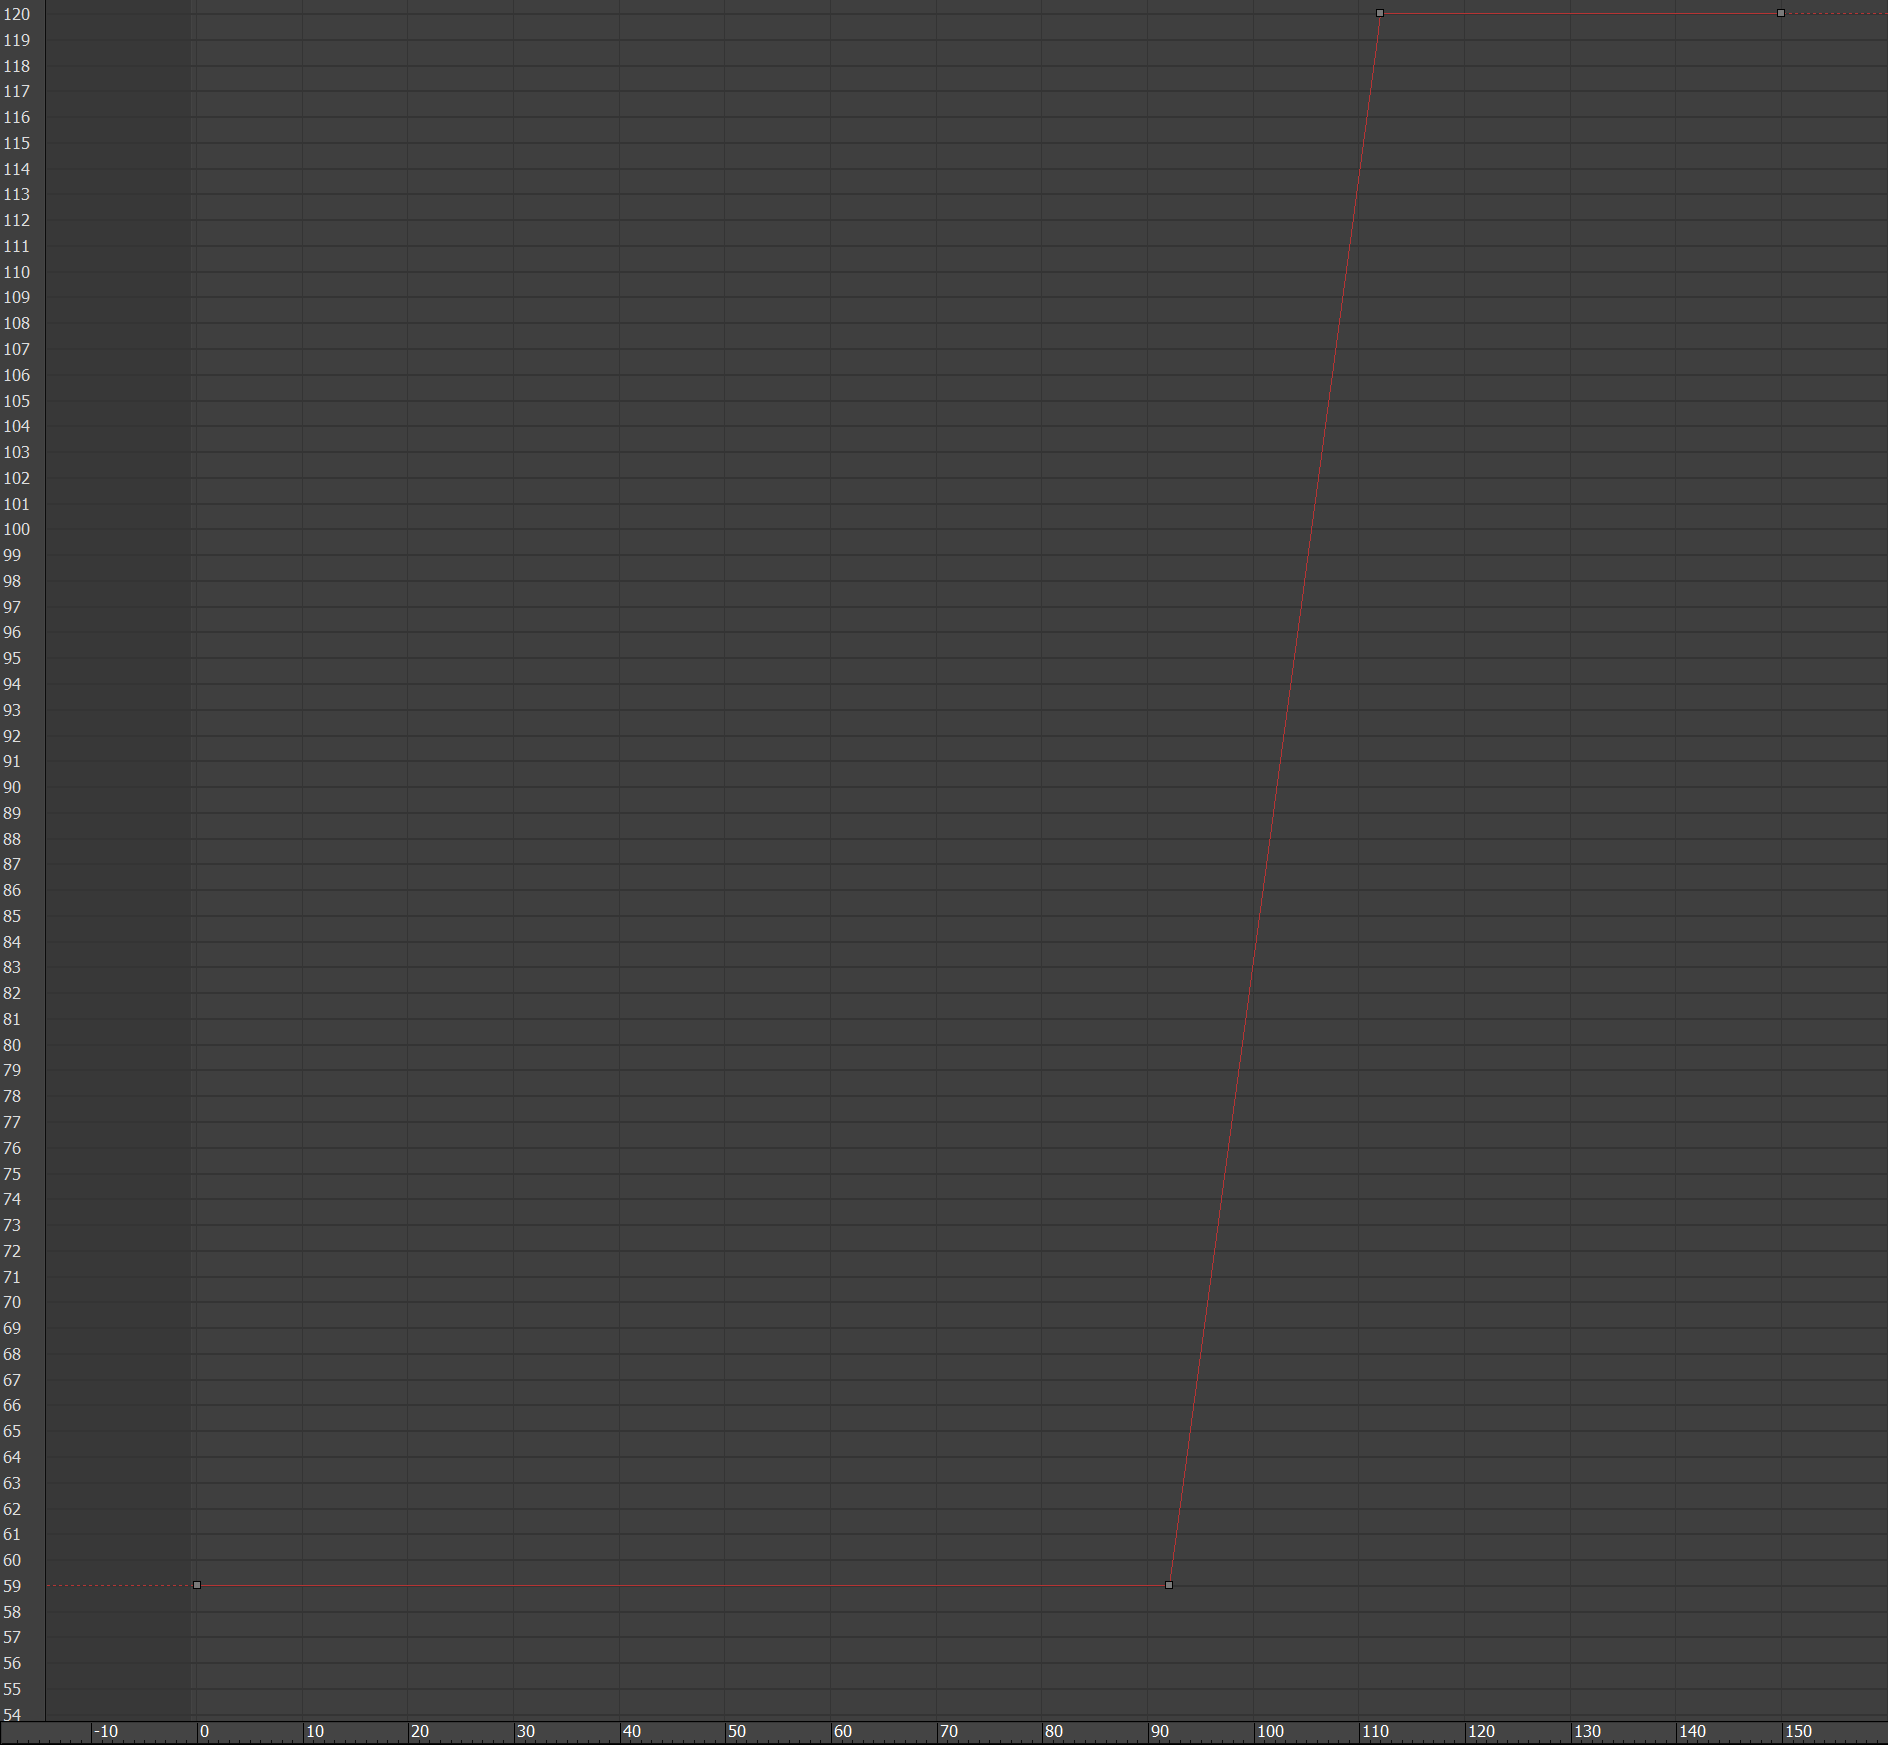
\includegraphics[width=0.6\textwidth]{imagenes/curvas/PR/pelota/red.png}
    \caption{Curva que representa la posición en el eje X con respecto el tiempo.}
 \end{figure}

Esta curva representa la posición en el eje X con respecto al tiempo. Ocurre de manera similar que con la pelota izquierda, he utilizado una función lineal porque era la que me parecía más realista.

\bigskip

Mientras que los \textit{keyframes} para su \textit{Dummy} son:

\begin{itemize}
    \item \textbf{Instante 0: }El \textit{Dummy} se encuentra rotado para que la pelota se encuentre sobre el trampolín. Al igual que con la pelota, se debe hacer para que la animación inversa se haga al mismo tiempo.
    \item \textbf{Instante 58: }No ha habido cambios en la animación, es igual que el instante anterior.
    \item \textbf{Instante 92: }Ahora el \textit{Dummy} se encuentra rotado en la posición original; es decir, sin ninguna rotación aplicada para que la trayectoria de la pelota sea correcta.
    \item \textbf{Instante 150: }Ningún cambio realizado, solo es para que la animación inversa comience a la misma vez.
\end{itemize}

\newpage

La curva de animación para el \textit{Dummy} es:

\begin{figure}[H]
    \centering
    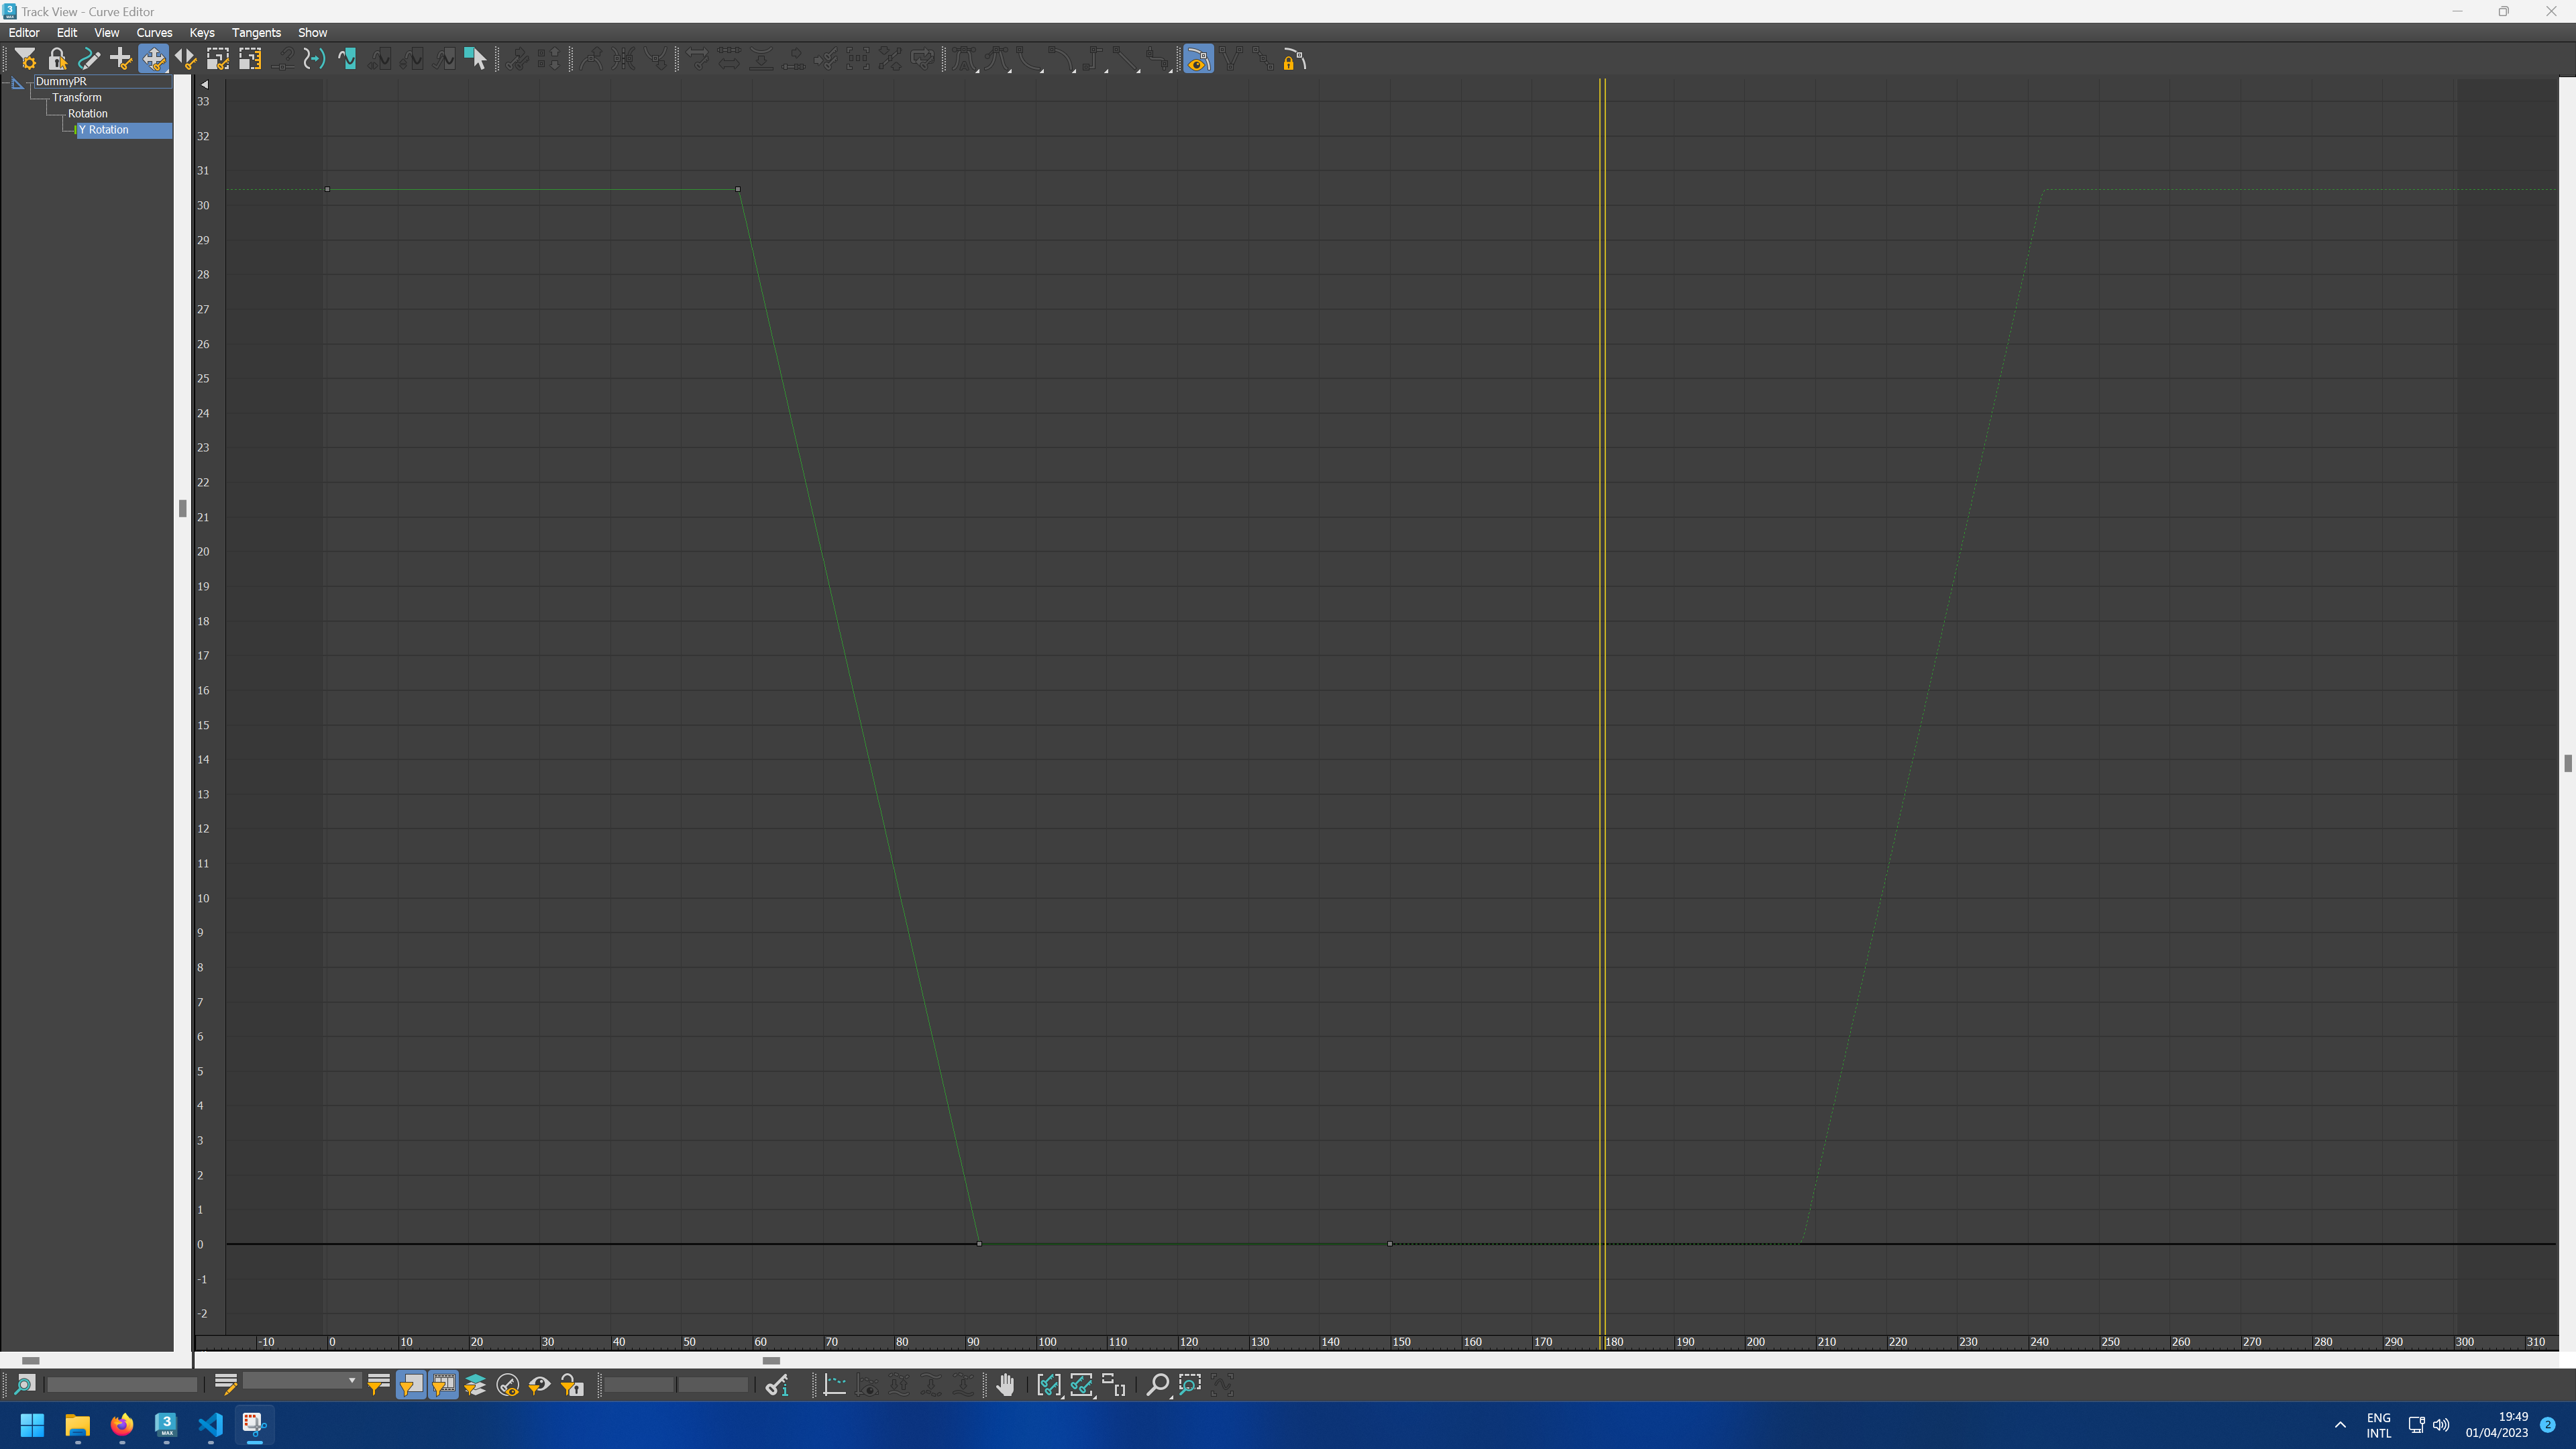
\includegraphics[width=0.6\textwidth]{imagenes/curvas/PR/dummy/green.png}
    \caption{Curva que representa la rotación en el eje Y con respecto el tiempo.}
 \end{figure}

De nuevo, ocurre de manera similar que con el \textit{Dummy} de la otra pelota. La curva es lineal, ya que la pelota le transfiere al trampolín toda la energía potencial que tenía, haciendo que no tenga tiempo de acelerar y se ponga a la velocidad máxima directamente.

\bigskip

Además, esta pelota sigue el mismo espaciado en los \textit{keyframes} que la otra, pero comenzando desde el instante 150 y hacia la izquierda; es decir, es como si fuera un ``reflejo'' de la otra. Esto resultará en que la pelota comience sobre el trampolín y acabe dando saltos sobre la plataforma, así se puede repetir la animación inversa de manera fluida.

\bigskip

La pelota y su \textit{Dummy} se encuentran en la escena de la siguiente forma:

\begin{figure}[H]
   \centering
   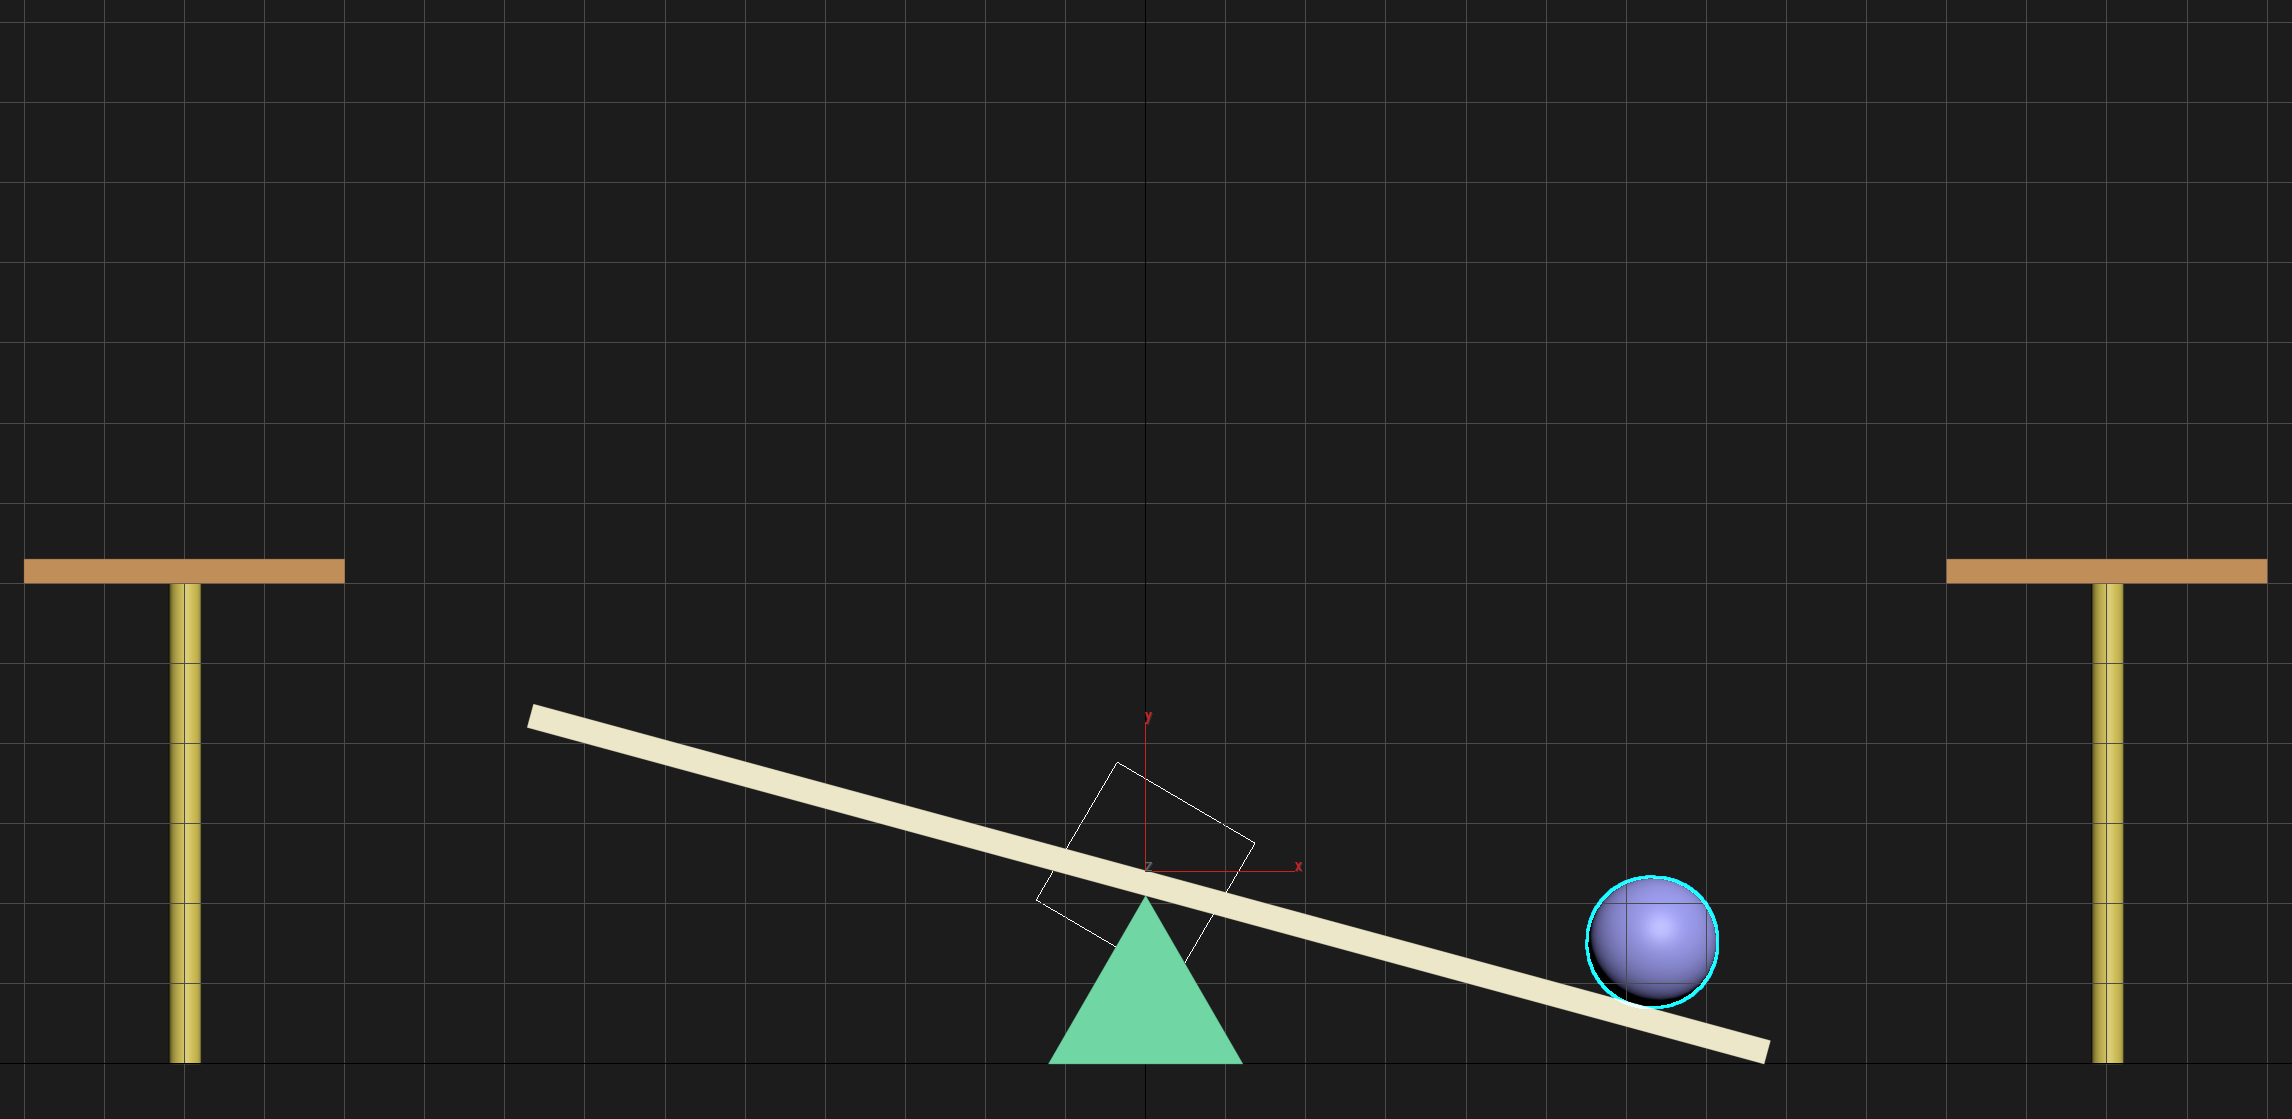
\includegraphics[width=0.7\textwidth]{imagenes/misc/PRDummy.png}
   \caption{Pelota derecha junto a su \textit{Dummy}.}
\end{figure}

\newpage
\subsection{Trampolín}
Para realizar el giro de la curva del trampolín es necesario sincronizar los instantes iniciales y finales de los \textit{dummies} de las pelotas, para que giren conjuntamente.

\bigskip

Los \textit{keyframes} para realizar la animación del trampolín son los siguientes:

\begin{itemize}
    \item \textbf{Instante 0: }Se encuentra girado hacia la derecha, con la pelota derecha sobre el trampolín. Como se ha dicho anteriormente, este instante es para sincronizar las animaciones con la parte en la que se realiza de forma inversa.
    \item \textbf{Instante 58: }Exactamente igual que el anterior instante.
    \item \textbf{Instante 92: }El trampolín ahora se encuentra girado hacia el otro lado debido a la energía que le transfiere la pelota izquierda.
    \item \textbf{Instante 150: }No varía nada de la animación con respecto al instante anterior. Ocurre exactamente igual que en el instante 0.
\end{itemize}

\bigskip

Y la curva de animación es:

\begin{figure}[H]
    \centering
    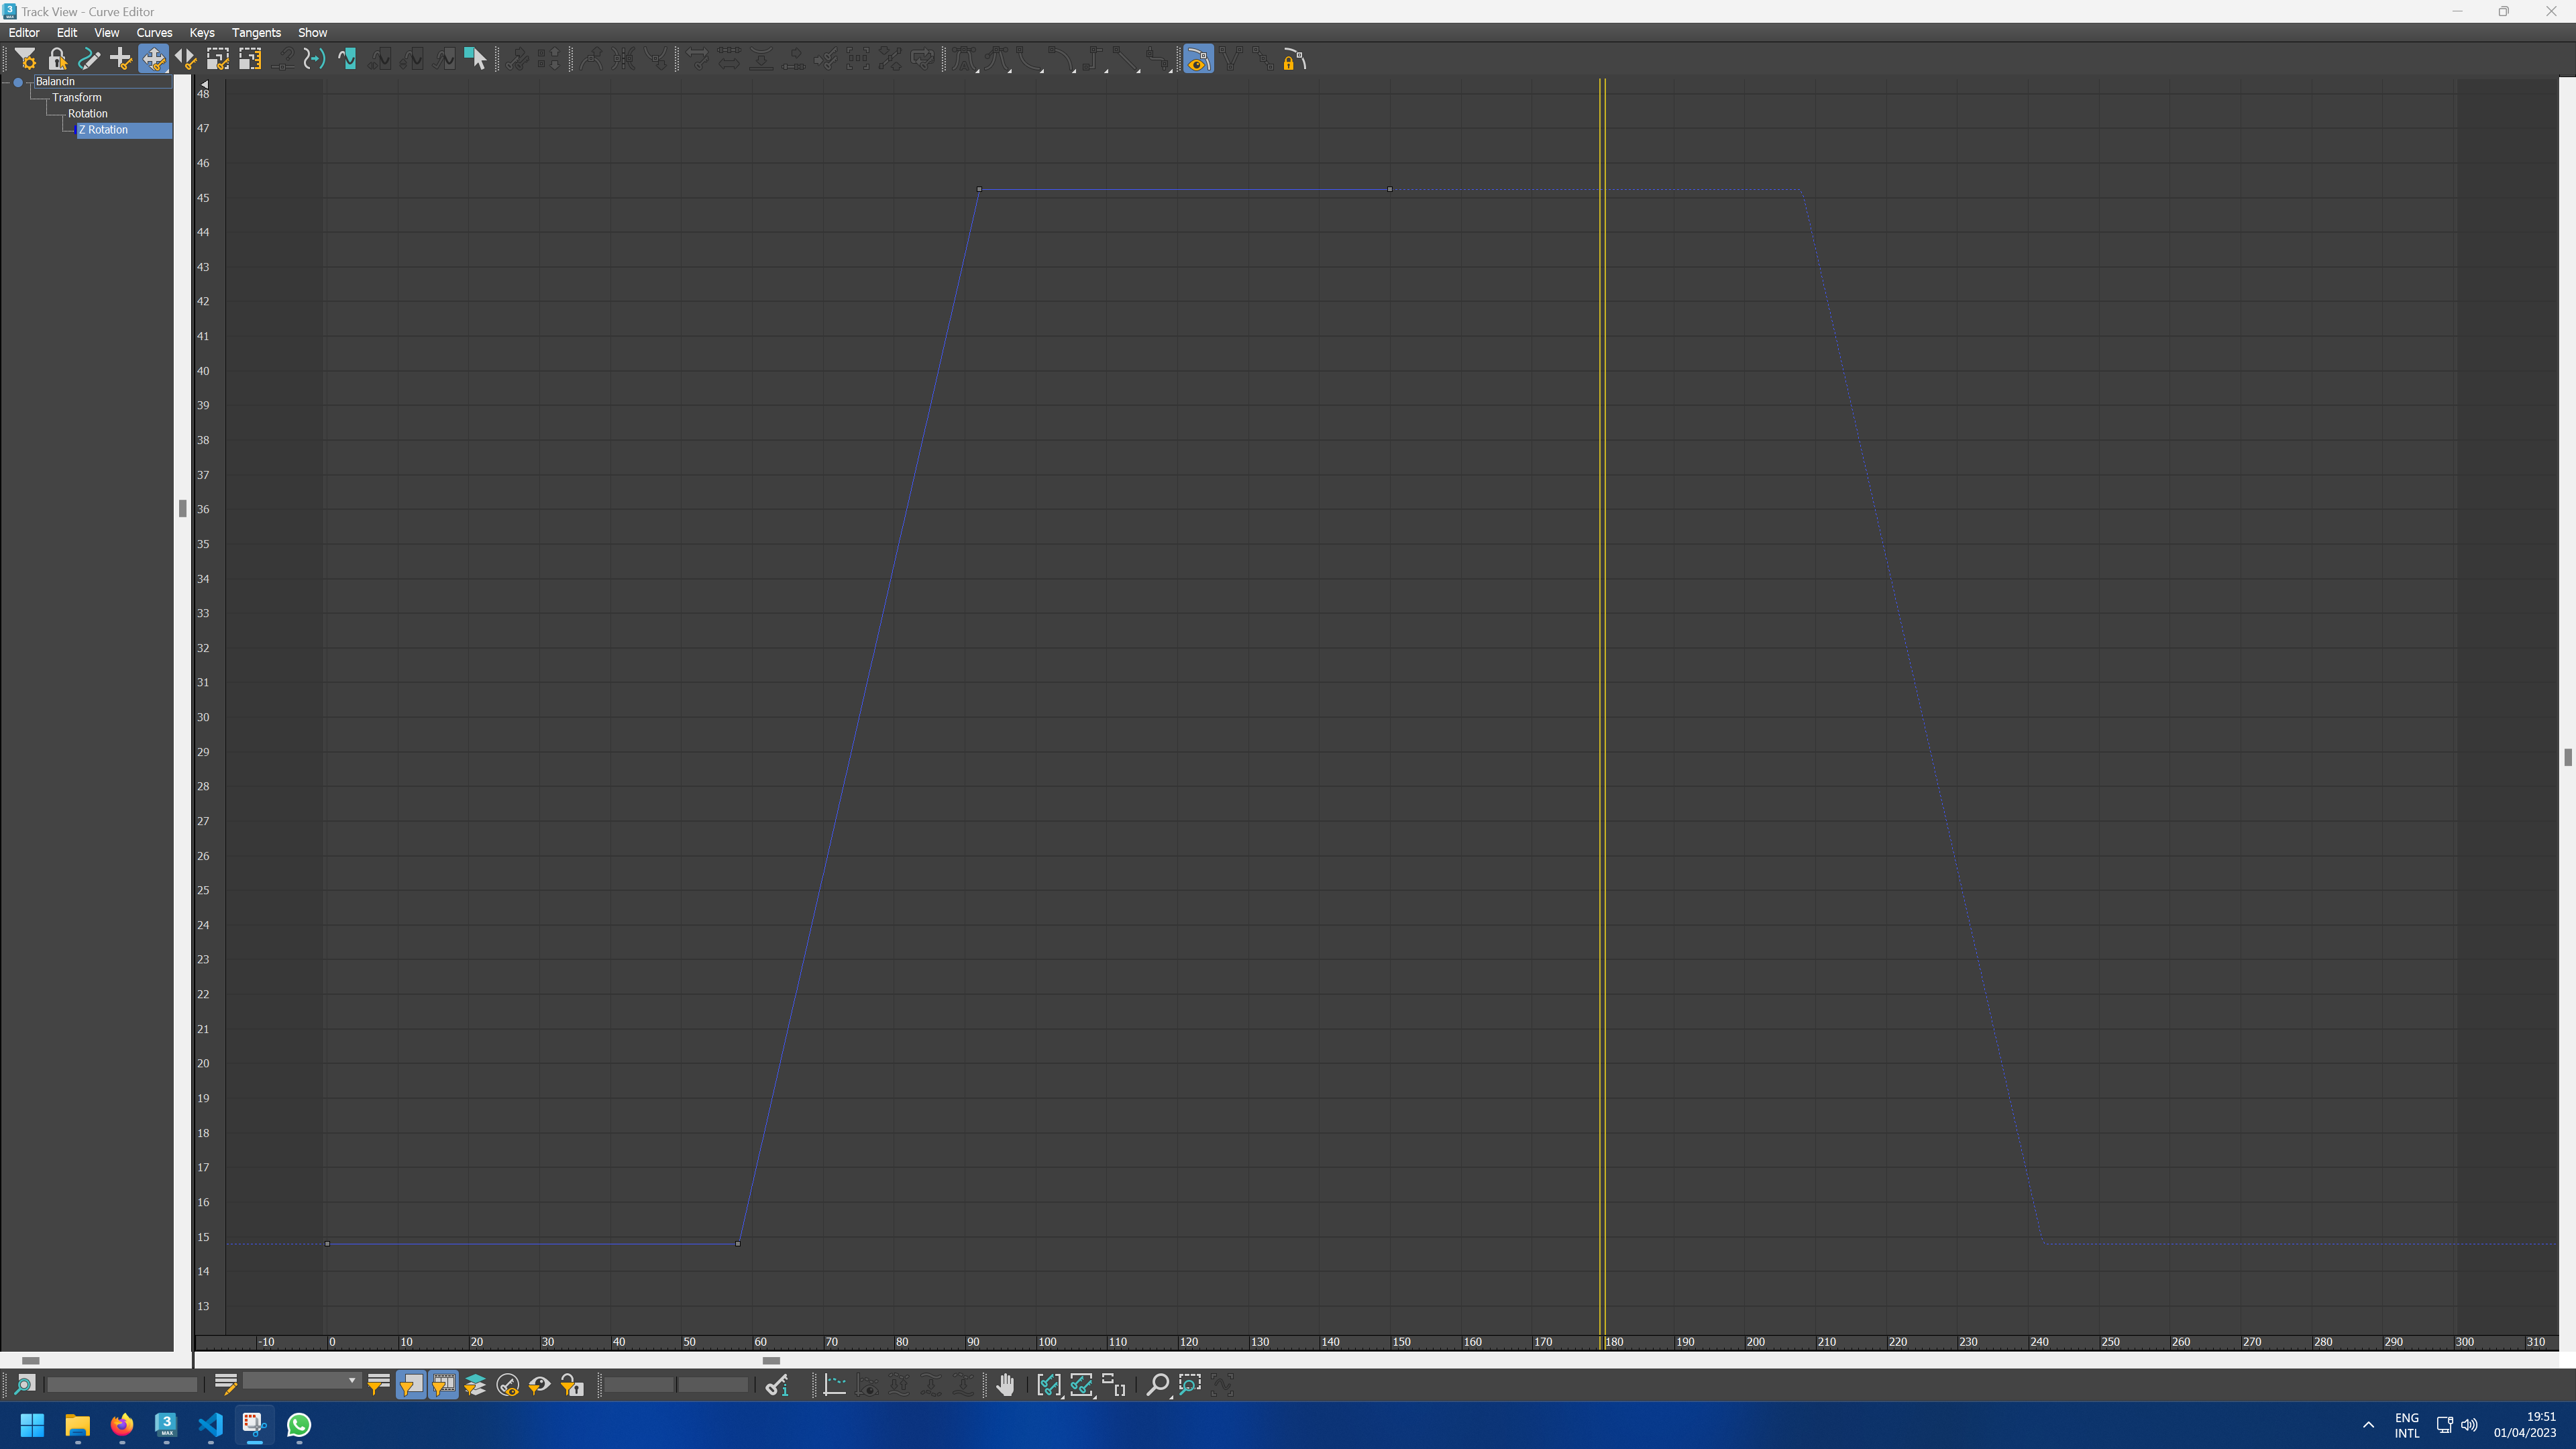
\includegraphics[width=0.6\textwidth]{imagenes/curvas/Trampolin/blue.png}
    \caption{Curva que representa la rotación en el eje Z con respecto al tiempo.}
 \end{figure}

 Al igual que las pelotas, como el balancín es hijo del punto de apoyo, la rotación realmente se ve reflejada en el eje Y en coordenadas del mundo, ya que el padre actúa de manera similar a los \textit{dummies}. Al igual que estos, el trampolín utiliza una curva lineal, ya que la energía potencial de la pelota que se encuentra en el aire, al tocarlo se la transfiere, sin la posibilidad de que acelere poco a poco.

 \newpage
\section{Iluminación de la escena}
Para la iluminación de la escena he utilizado una combinación de 3 luces, como se pedía en el guion, y de un cambio del color de fondo para que las zonas que no son iluminadas sean visibles.

\bigskip

Voy a dividir en subsecciones las explicaciones del color de fondo y de la iluminación:

\subsection{Color de fondo}

% rescribir
El color de fondo por defecto que tienen las escenas es el negro, haciendo que cuando se utiliza iluminación, las zonas no iluminadas por los puntos de luz aparezcan negros por completo. Para solucionar esto es necesario modificar el color de fondo por un gris oscuro, para que se pueda ver toda la escena.

\bigskip

Para ello, es necesario irse a los menús de arriba y darle clic a ``Rendering'' $\rightarrow$ ``Environment''.

\begin{figure}[H]
    \centering
    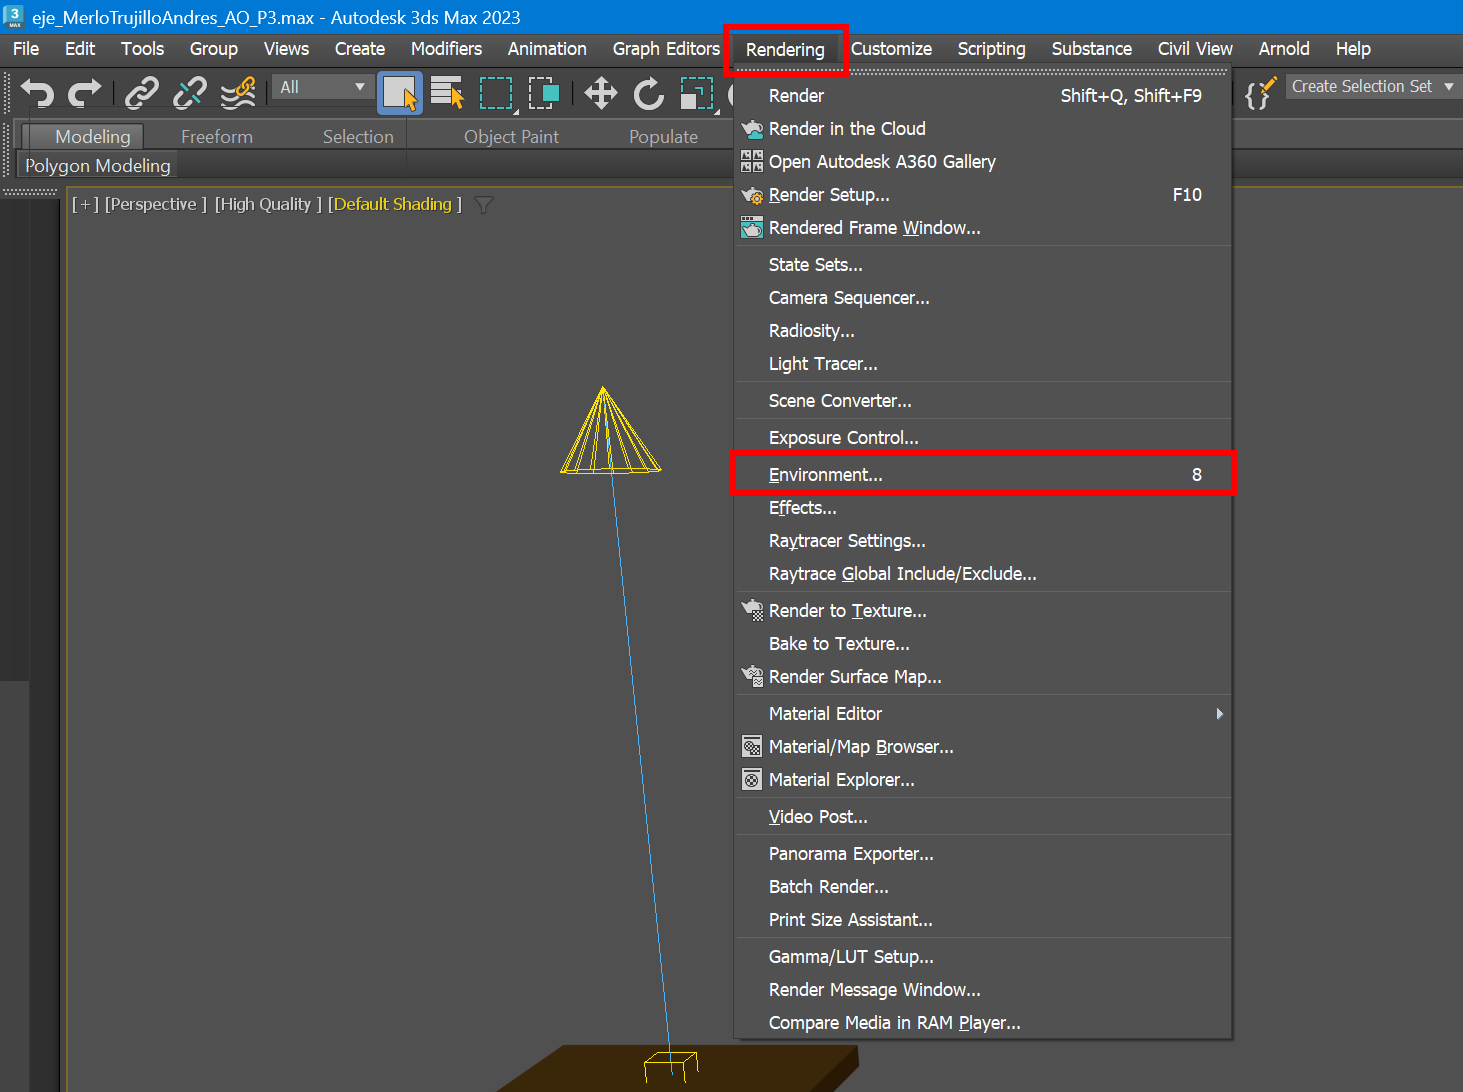
\includegraphics[width=0.7\textwidth]{imagenes/misc/bg-color1.png}
    \caption{Ubicación de la opción para cambiar el color de fondo.}
 \end{figure}

Se abrirá una ventana a la que hay que darle al rectángulo de selección de color de la sección ``Background'' y elegir un tono más claro.

\begin{figure}[H]
    \centering
    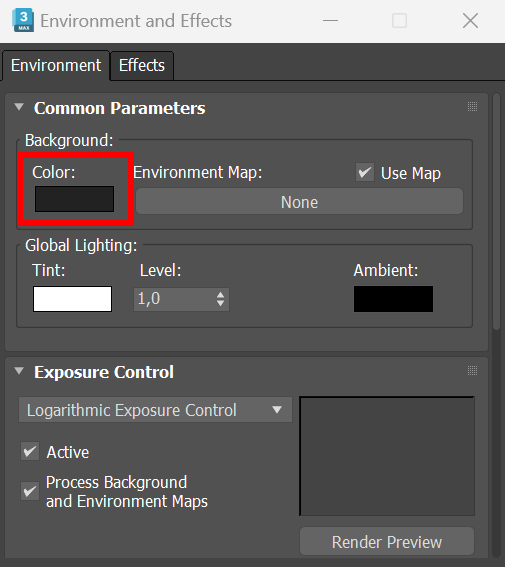
\includegraphics[width=0.5\textwidth]{imagenes/misc/bg-color2.png}
    \caption{Ventana con la opción para cambiar el color de fondo.}
 \end{figure}

\subsection{Puntos de luz de la escena}
Para la iluminación de la escena he utilizado 3 \textit{Target Lights} junto a una distribución de luz de tipo \textit{Spotlight}, permitiéndome modificar el cono de luz para que solo ilumine las bases, para el caso de las luces de los extremos, y el trampolín, para el caso de la luz intermedia.

\bigskip

Esta subsección la voy a dividir a su vez en distintas subsecciones, una para cada luz puesta en la escena.

\subsubsection{Luz de la izquierda}
% rescribir

Los \textit{keyframes} para el foco de la izquierda son:

\begin{itemize}
    \item \textbf{Instante 0: }La luz ahora mismo se encuentra encendida y de color blanco. Se hace para que la animación inversa funcione correctamente.
    \item \textbf{Instante 38: }La luz se encuentra exactamente igual que en el instante anterior.
    \item \textbf{Instante 58: }La luz pasa a tener color rojo y apagarse (intensidad a 0) porque la pelota ha saltado de la plataforma.
    \item \textbf{Instante 150: }Exactamente igual que en el instante anterior. Se realiza para hacer que la animación inversa funcione bien y porque la pelota no está en la base.
\end{itemize}

\newpage

Las curvas de animación son las siguientes:

\begin{figure}[H]
    \centering
    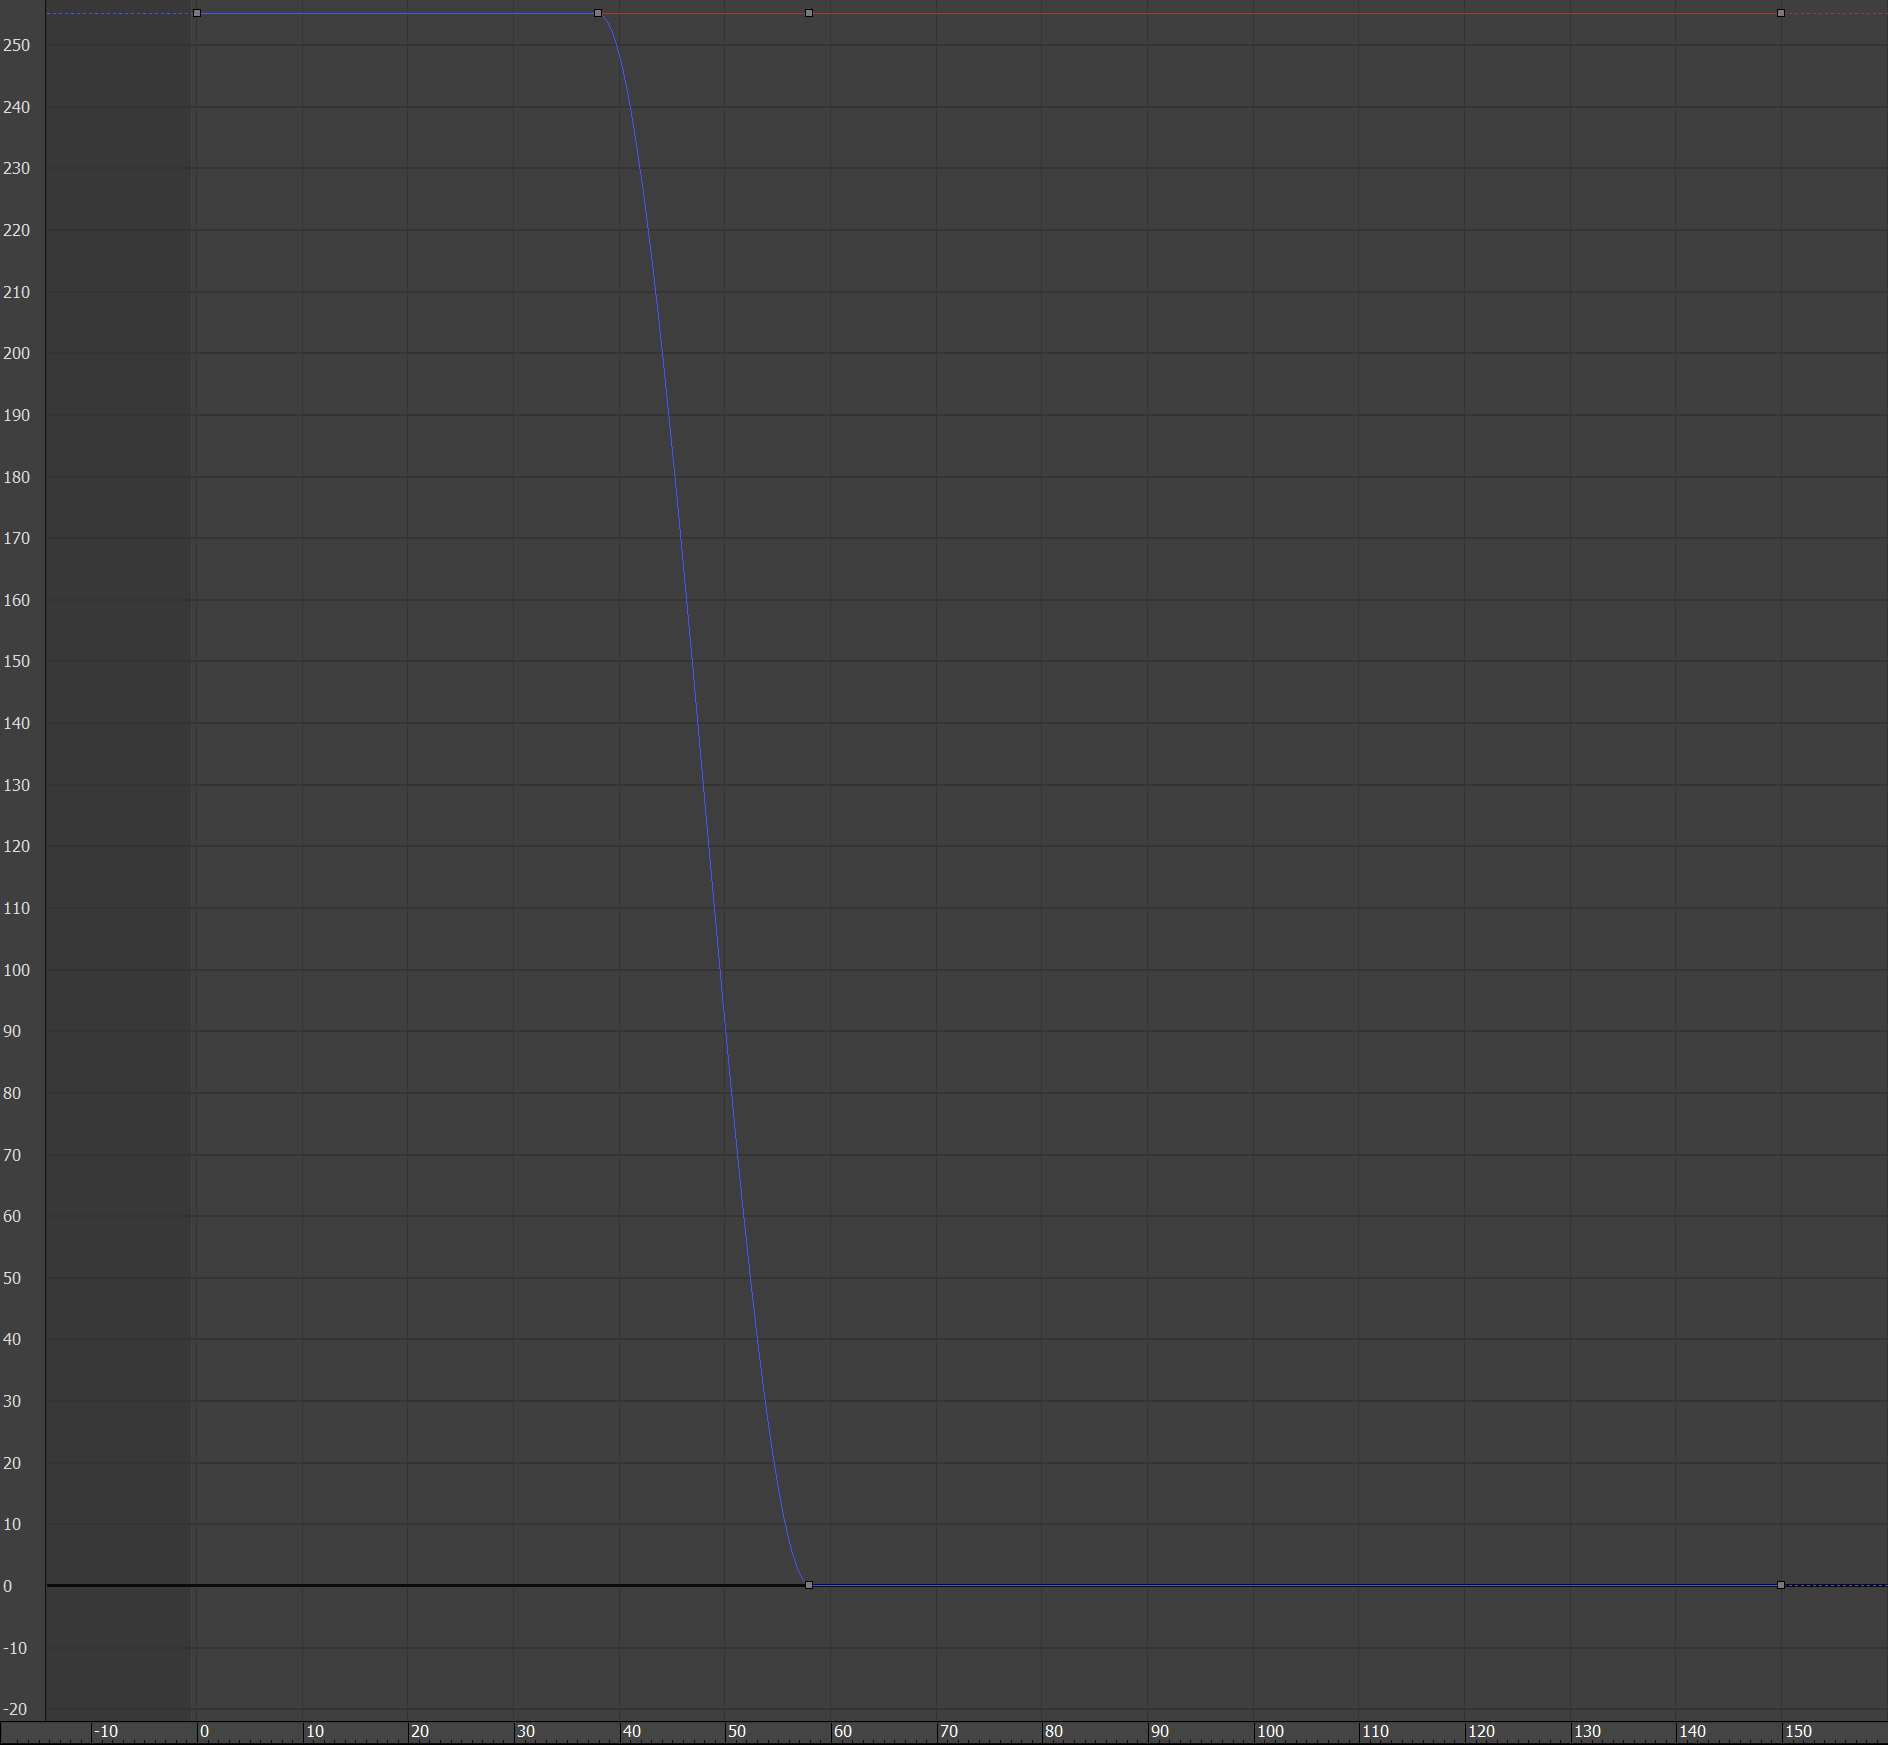
\includegraphics[width=0.6\textwidth]{imagenes/curvas/LL/filter.png}
    \caption{Curva que representa el color de la luz con respecto al tiempo.}
 \end{figure}

En la curva he usado una función \textit{Slow-in/Slow-out} para simular la iluminación progresiva que tendría una luz incandescente al ser encendidas y apagada.

 \begin{figure}[H]
    \centering
    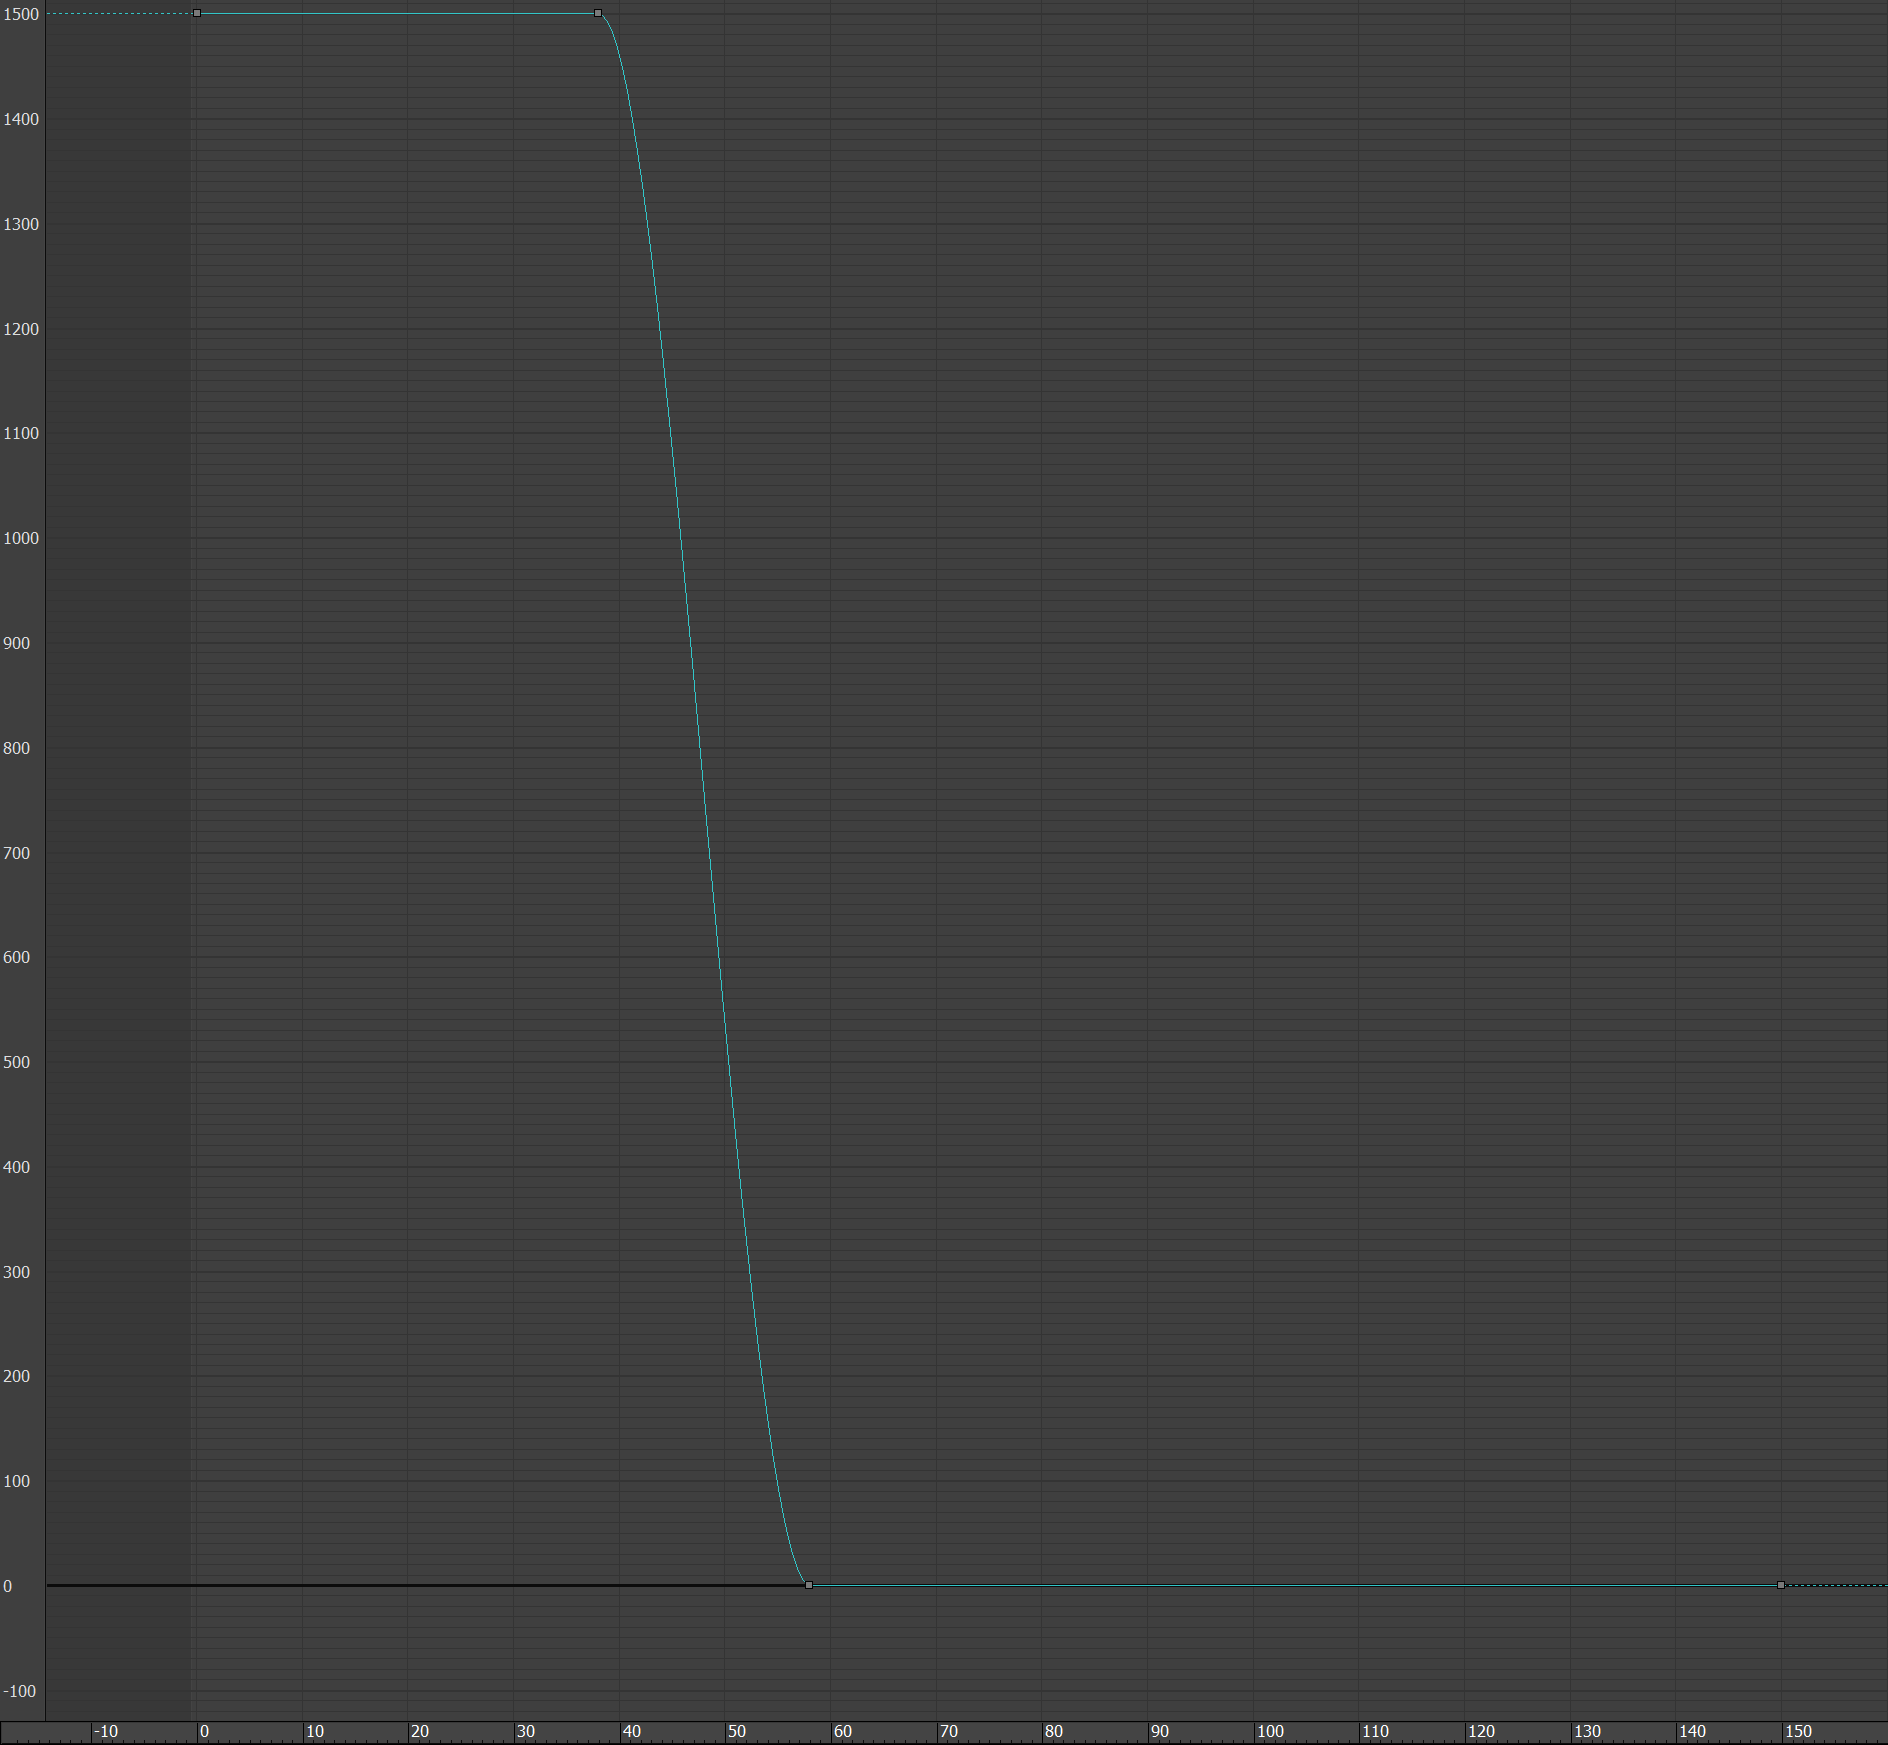
\includegraphics[width=0.6\textwidth]{imagenes/curvas/LL/intensity.png}
    \caption{Curva que representa la intensidad de la luz con respecto al tiempo.}
 \end{figure}

 En esta curva también he usado el mismo tipo de función que en la anterior, con el objetivo de simular el encendido y apagado progresivo que tienen algunas luces, entre ellas las incandescentes como antes.

 \subsubsection{Luz de la derecha}

 El punto de luz del otro extremo que ilumina la otra pelota tiene los mismos \textit{keyframes}, pero comenzando desde el final:

 \begin{itemize}
    \item \textbf{Instante 0: }Se encuentra de color rojo y con la intensidad a 0. Esto se hace para que la animación inversa funcione de manera correcta con las demás componentes y porque no se encuentra la pelota en la base.
    \item \textbf{Instante 92: }La luz sigue exactamente igual que en el instante anterior.
    \item \textbf{Instante 112: }La luz ahora se encuentra iluminada al máximo y de color blanco.
    \item \textbf{Instante 150: }Se encuentra exactamente igual que en el instante anterior, con el objetivo de que la animación inversa funcione correctamente y porque la pelota está rebotando en la base.
 \end{itemize}
 
 \bigskip

Las curvas de animación son las siguientes:

\begin{figure}[H]
    \centering
    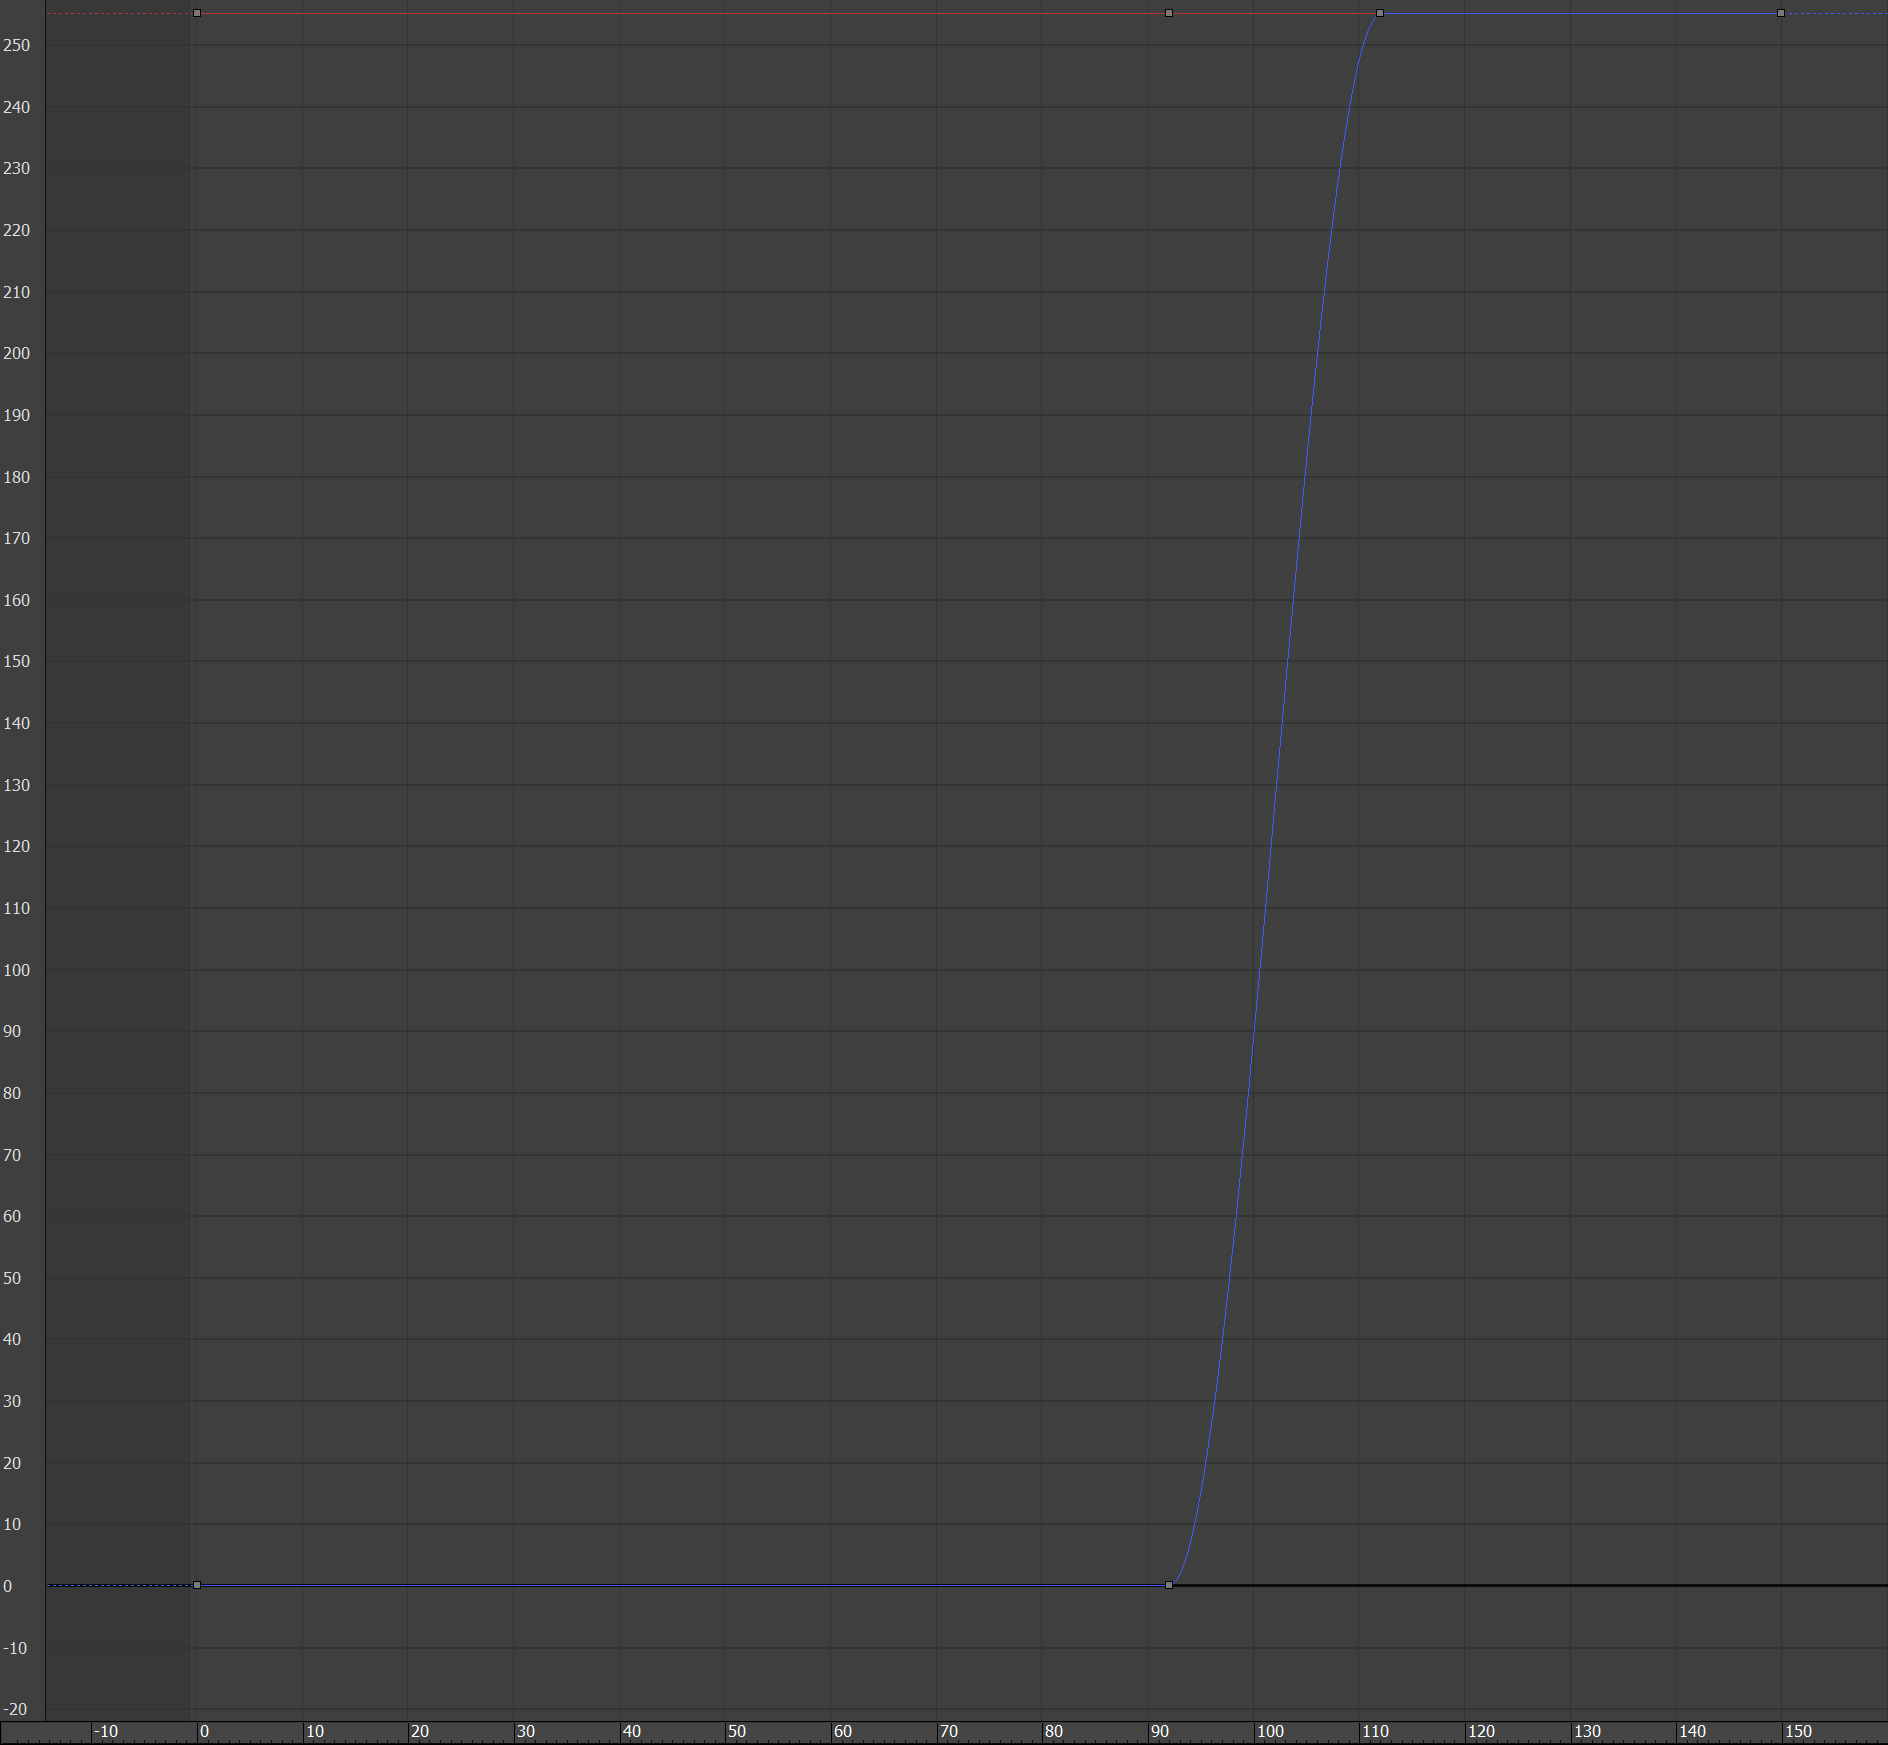
\includegraphics[width=0.6\textwidth]{imagenes/curvas/LR/filter.png}
    \caption{Curva que representa el color de la luz con respecto al tiempo.}
 \end{figure}

 \begin{figure}[H]
    \centering
    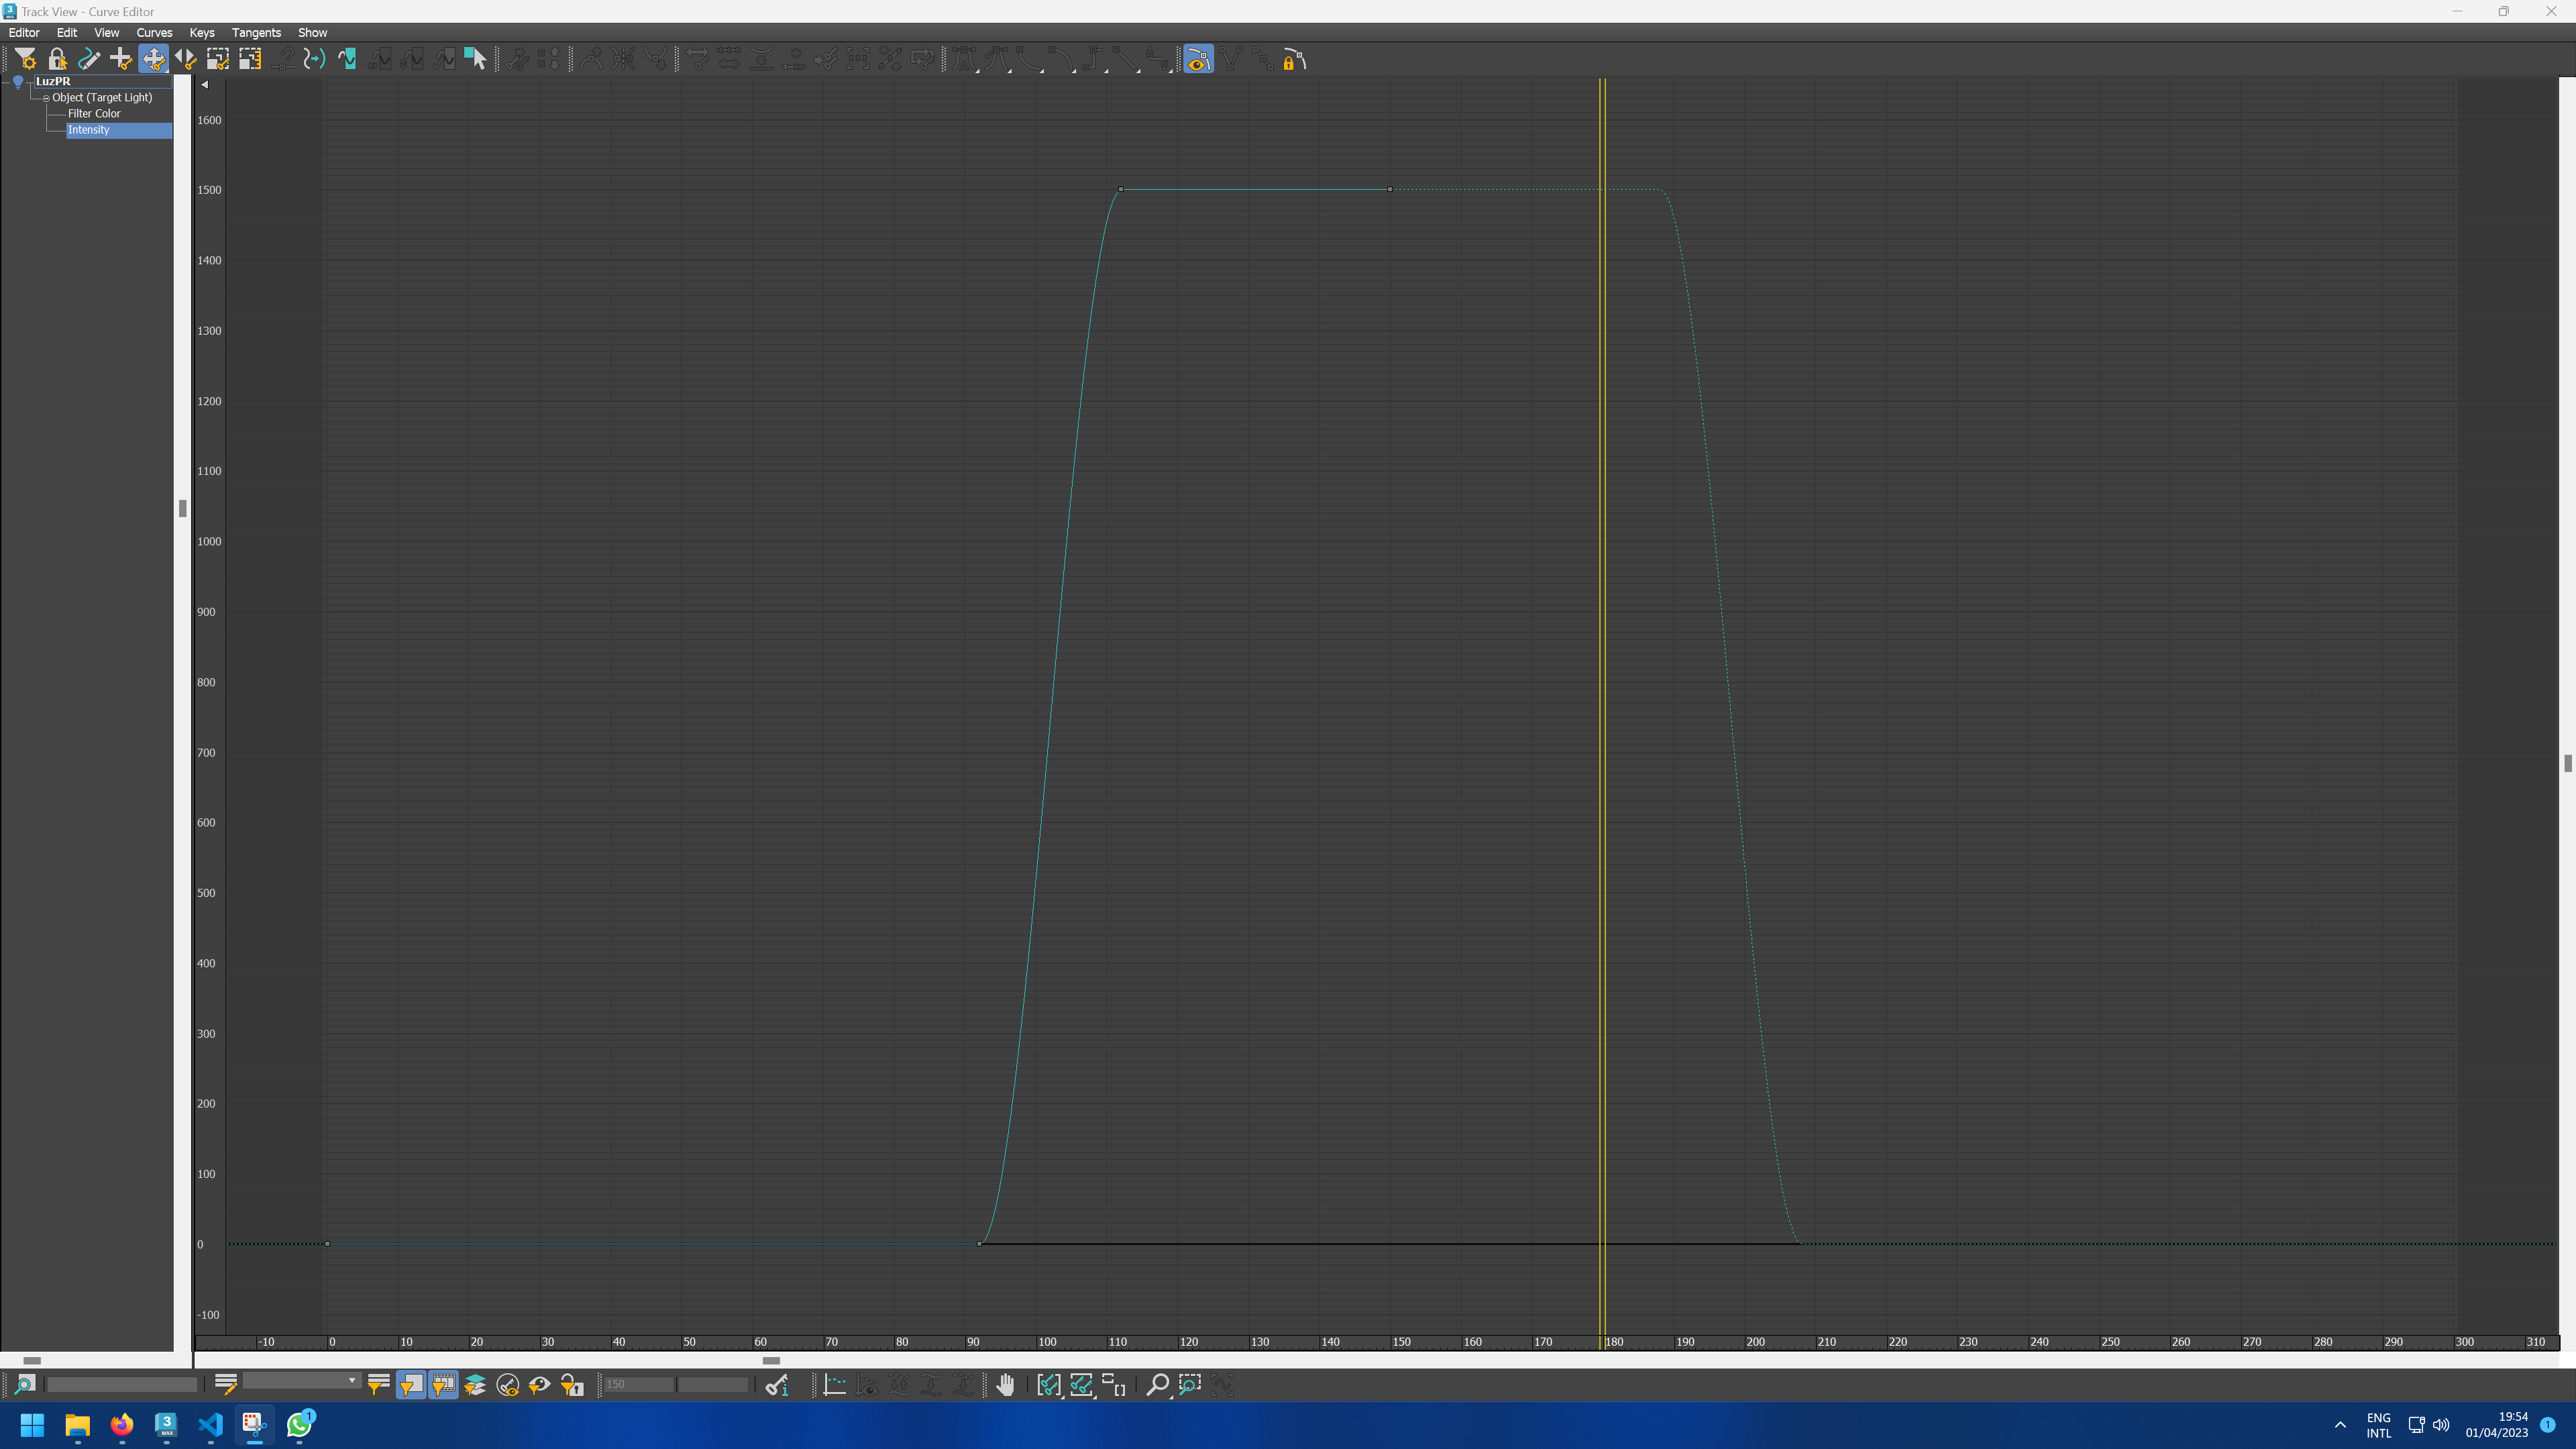
\includegraphics[width=0.6\textwidth]{imagenes/curvas/LR/intensity.png}
    \caption{Curva que representa la intensidad de la luz con respecto al tiempo.}
 \end{figure}

Al igual que con la luz del otro extremo, esta se encenderá y apagará progresivamente, simulando una luz incandescente.


\subsubsection{Luz central}

La luz intermedia, utilizada para iluminar el trampolín, tiene los siguientes \textit{keyframes}:

\begin{itemize}
    \item \textbf{Instante 0: }La luz se encuentra apagada y de color rojo, para hacer la animación inversa correctamente y porque no hay movimiento en el trampolín.
    \item \textbf{Instante 38: }La luz sigue exactamente igual que en el instante anterior.
    \item \textbf{Instante 58: }La luz se encuentra encendida y de color blanco, indicando que hay movimiento en el trampolín.
    \item \textbf{Instante 92: }La luz sigue exactamente igual que antes, ya que todavía hay movimiento en el trampolín.
    \item \textbf{Instante 112: }La luz ahora se encuentra apagada y de color rojo, al no haber más movimiento en el trampolín.
    \item \textbf{Instante 150: }Sigue sin haber movimiento, por lo que sigue apagada y de color rojo. También es para que la animación inversa funcione.
\end{itemize}

\newpage

Y las curvas de animación son:

\begin{figure}[H]
    \centering
    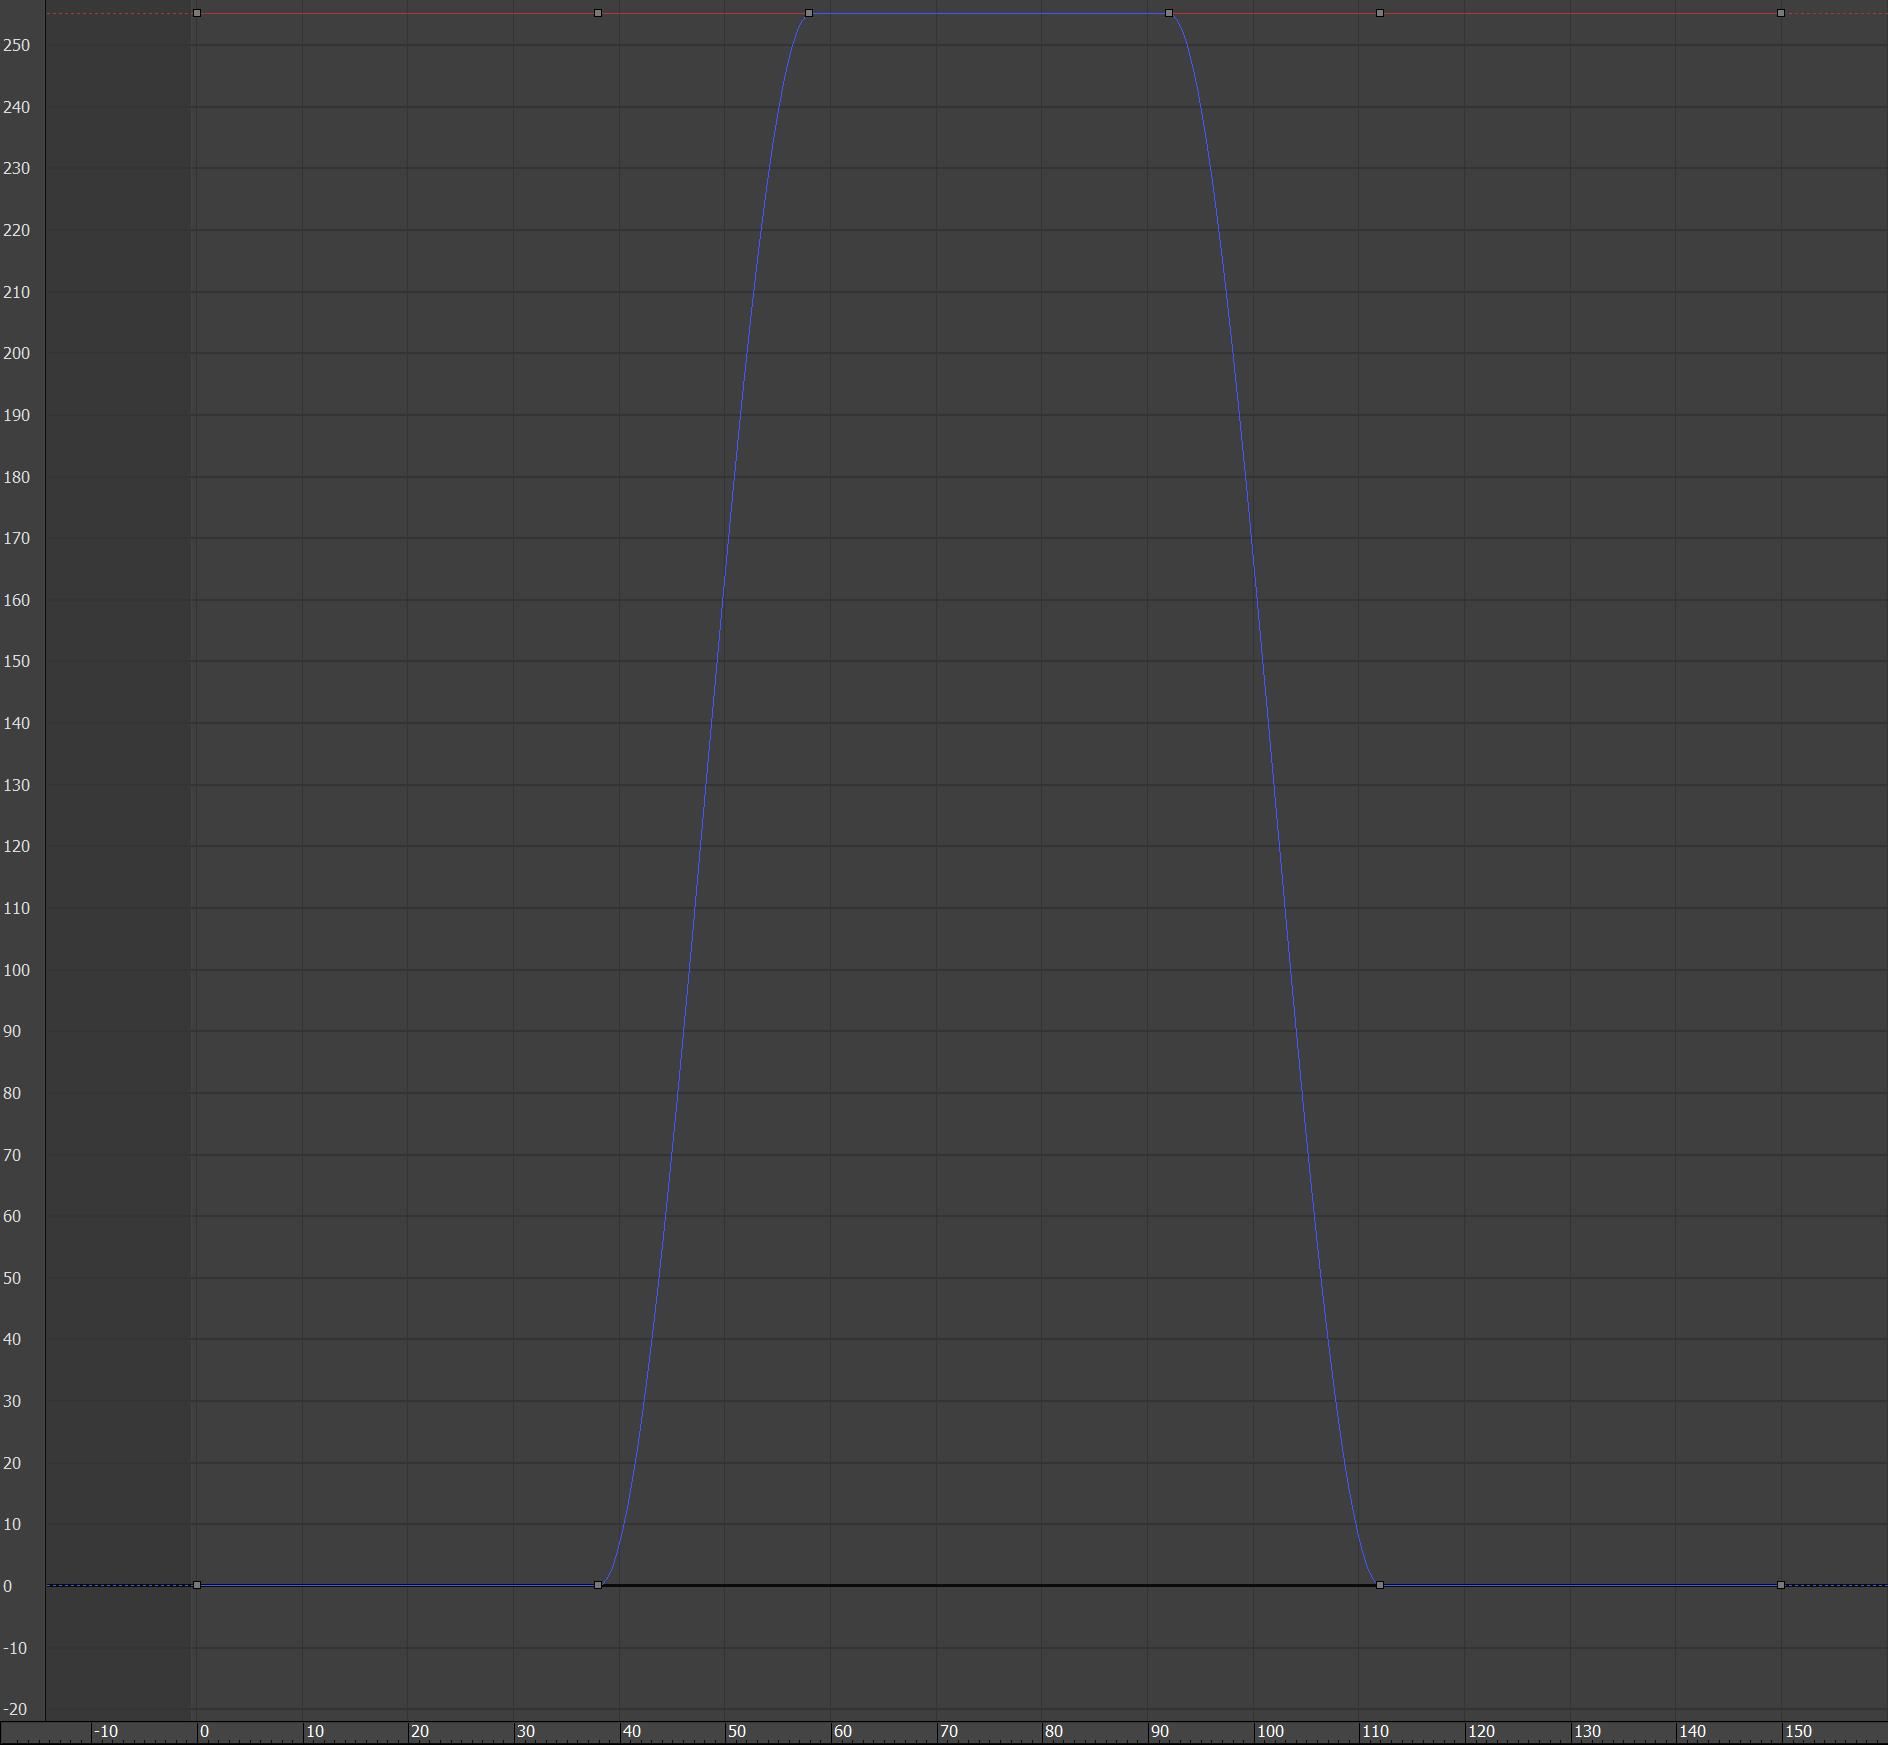
\includegraphics[width=0.6\textwidth]{imagenes/curvas/LC/filter.png}
    \caption{Curva que representa el color de la luz con respecto al tiempo.}
 \end{figure}

 \begin{figure}[H]
    \centering
    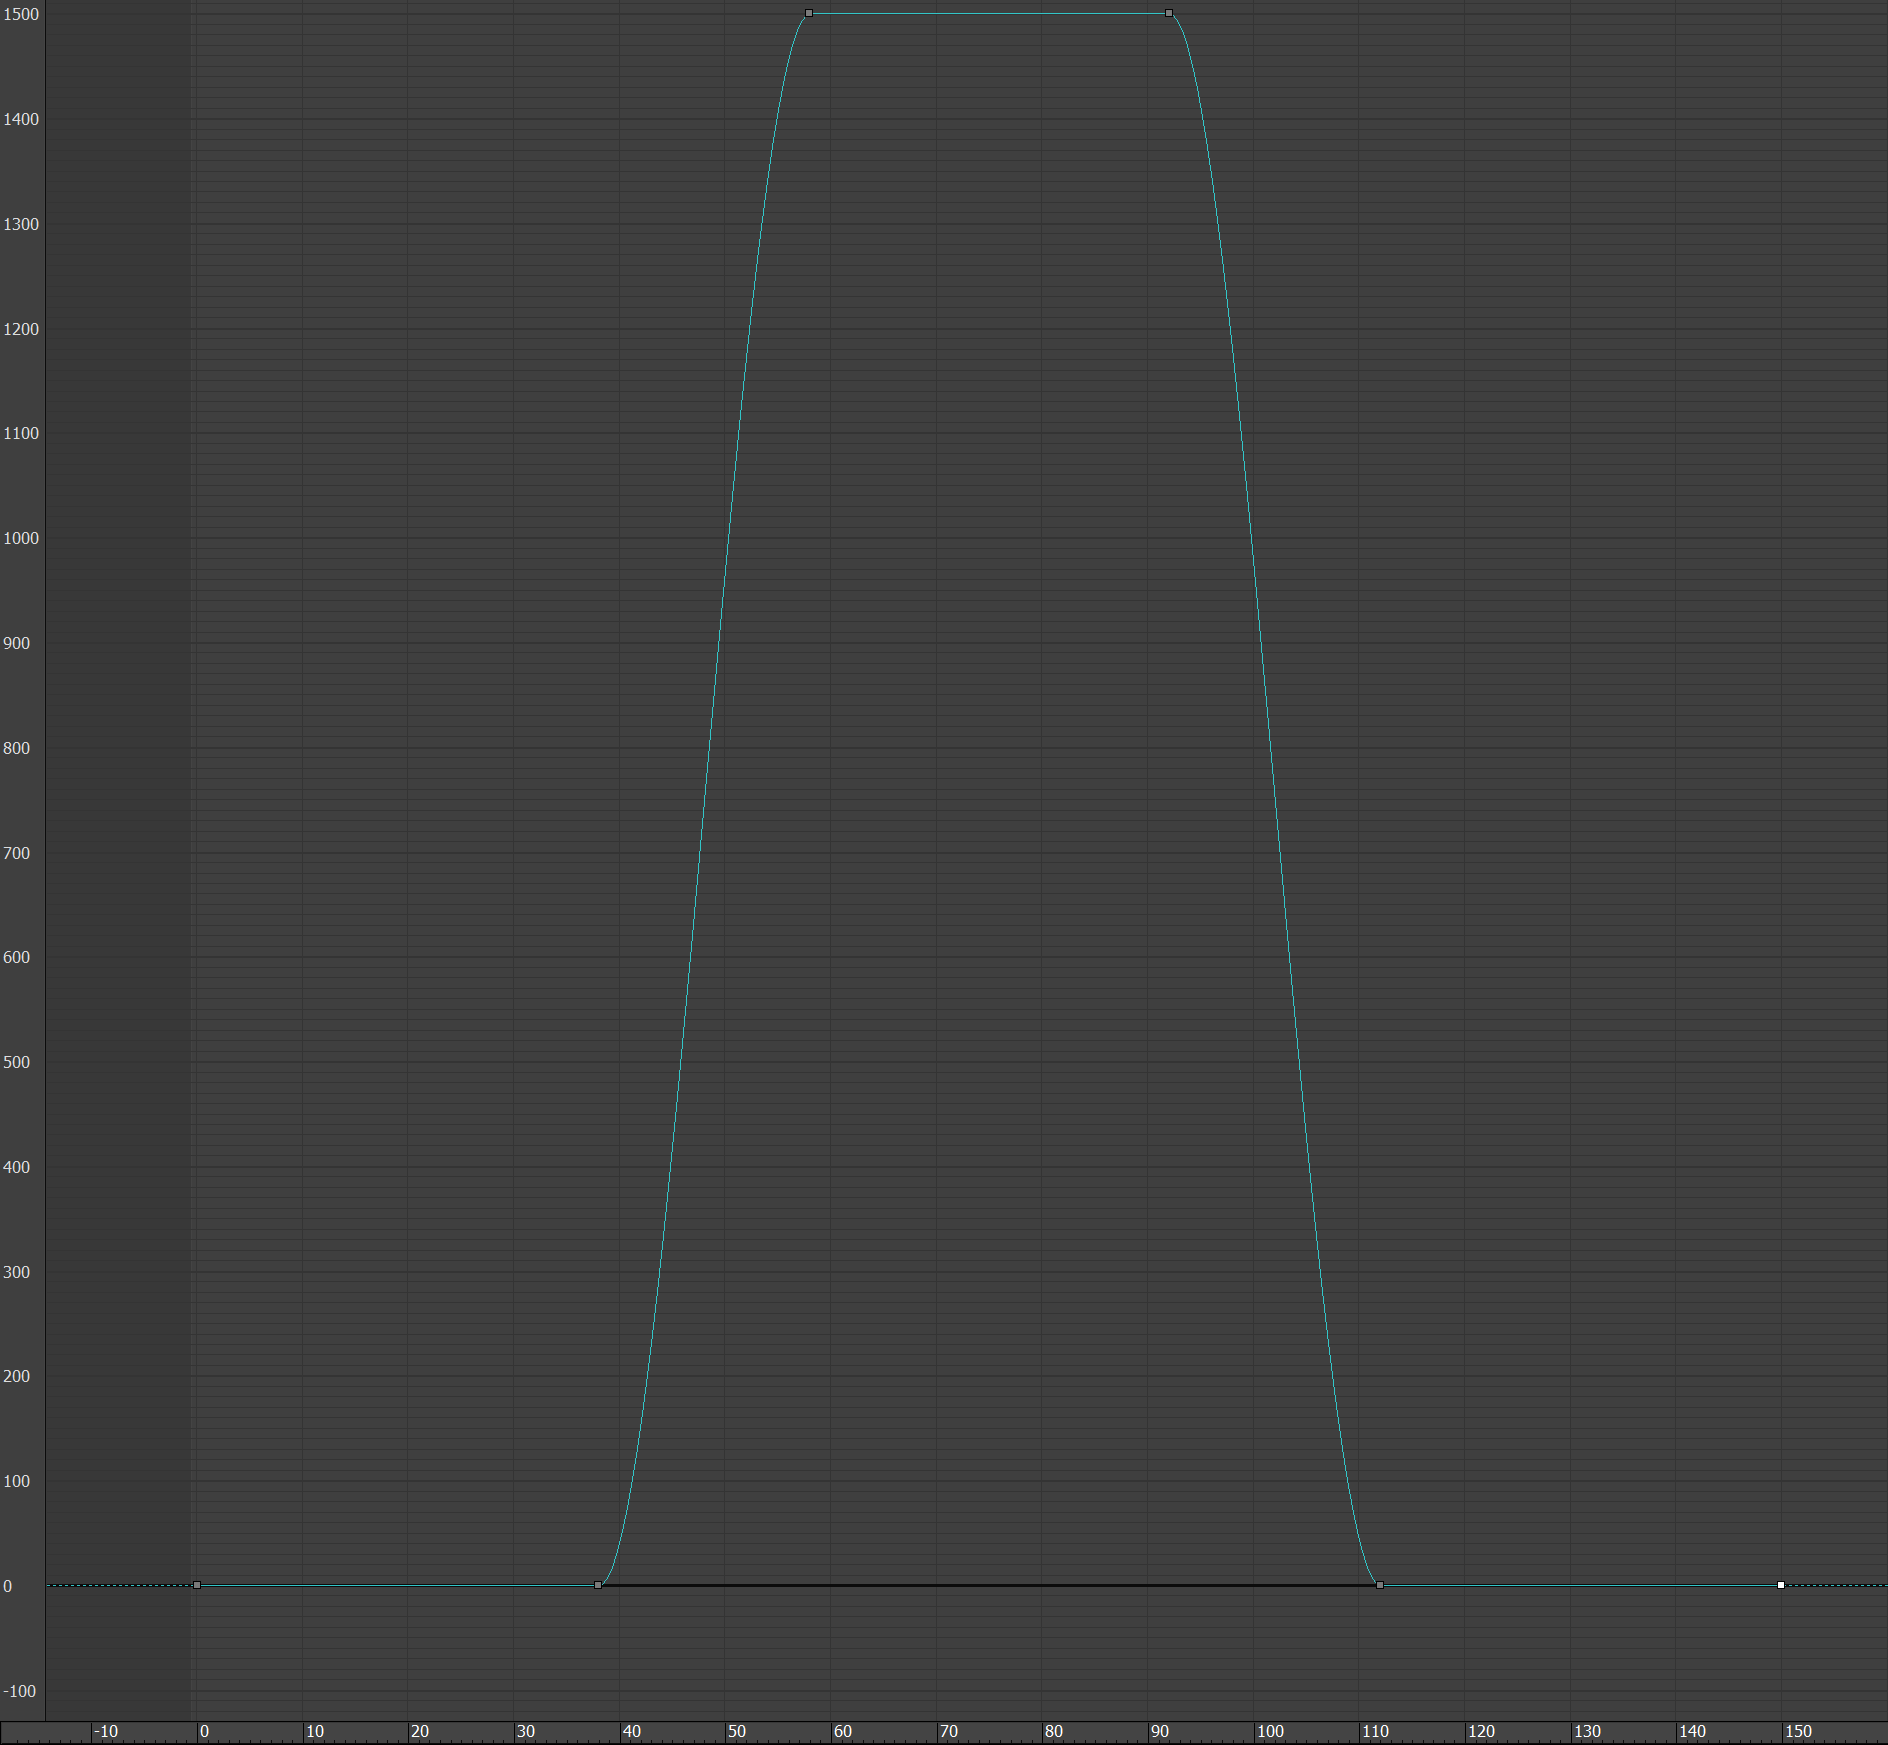
\includegraphics[width=0.6\textwidth]{imagenes/curvas/LC/intensity.png}
    \caption{Curva que representa la intensidad de la luz con respecto al tiempo.}
 \end{figure}

Al igual que con las otras luces, he utilizado una curva \textit{Slow-in/Slow-out} para simular el encendido y apagado progresivo de la luz.

\newpage

\section{Animación de la cámara}
Para animar el movimiento de la cámara he utilizado un \textit{Dummy} y he puesto como hijo a la propia cámara sin su \textit{Target}. Con esto, ya es posible animar el giro de la cámara sin demasiada complicación y permitiendo que siempre esté apuntando hacia la escena.

\bigskip

Los \textit{keyframes} de la cámara son:

\begin{itemize}
    \item \textbf{Instante 0: }La cámara se encuentra en la posición inicial, con una perspectiva similar a la que aparece en el guion.
    \item \textbf{Instante 150: }La cámara se encuentra en su posición final, que en este caso he decidido que sea la misma, para que haga una rotación completa en los 5 segundos.
\end{itemize}

\bigskip

La curva de animación del \textit{Dummy} de la cámara es:

\begin{figure}[H]
    \centering
    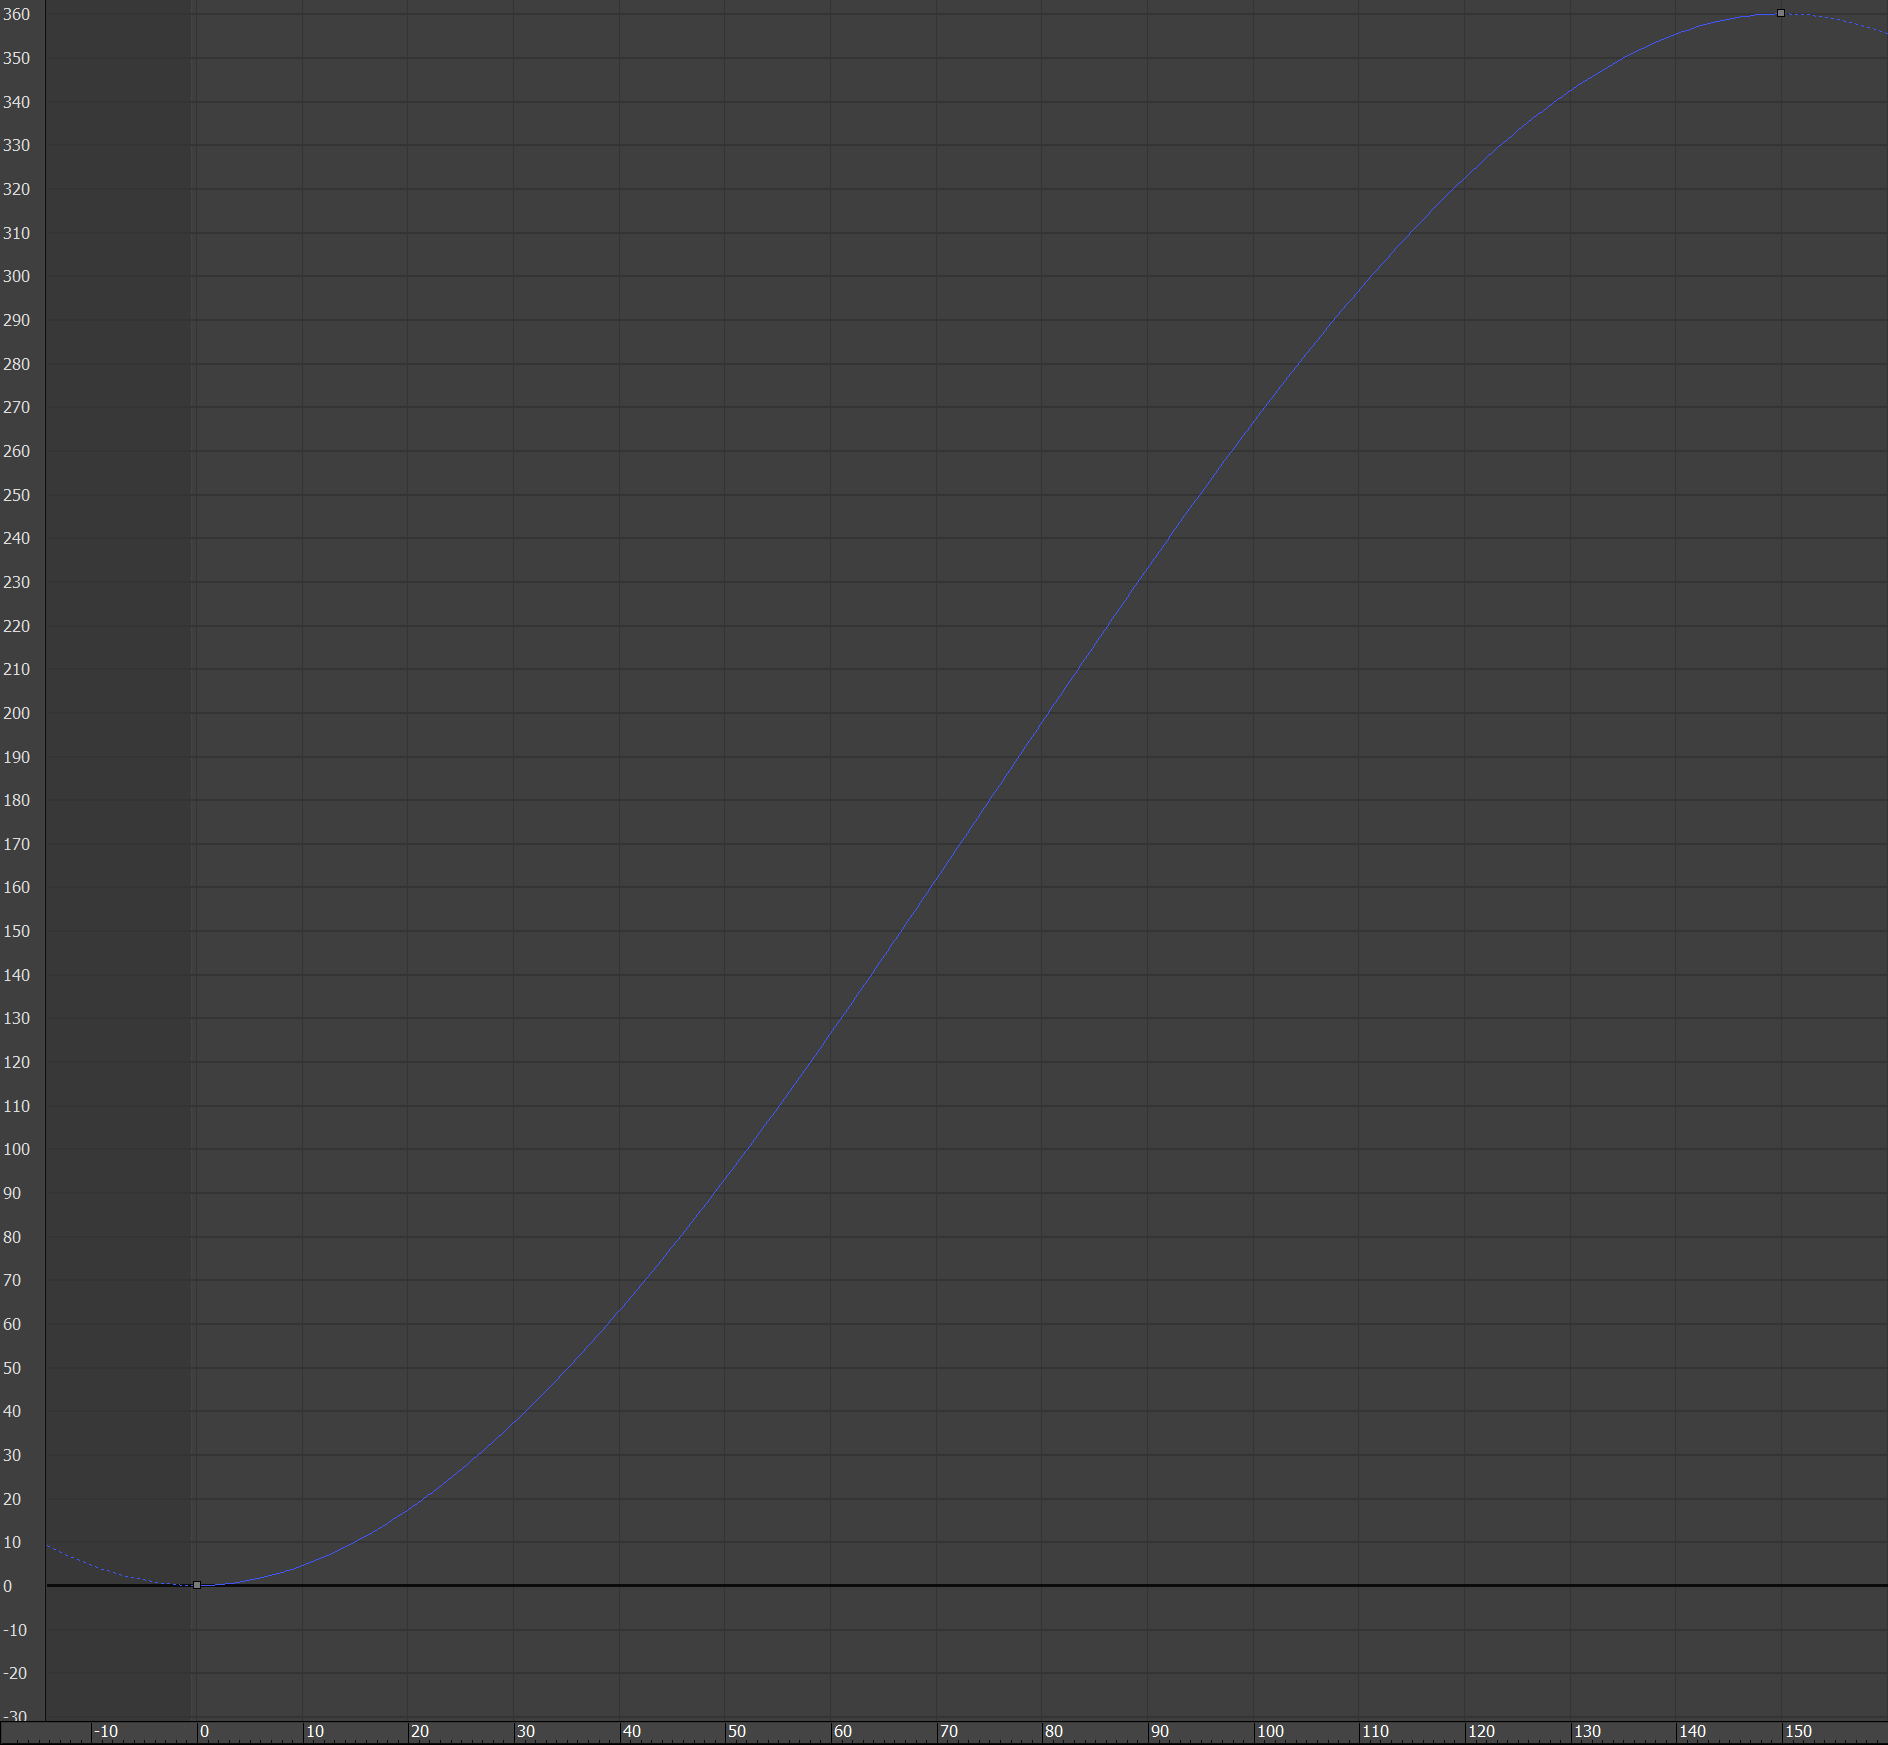
\includegraphics[width=0.6\textwidth]{imagenes/curvas/Camara/blue.png}
    \caption{Curva que representa la rotación en el eje Z con respecto al tiempo.}
 \end{figure}

Como se puede observar, he utilizado una función \textit{Slow-in/Slow-out}, para dar una sensación más realista al hacer la animación inversa, ya que de la otra forma parecía demasiado robótico.

\newpage

La trayectoria que sigue es la siguiente:

\begin{figure}[H]
   \centering
   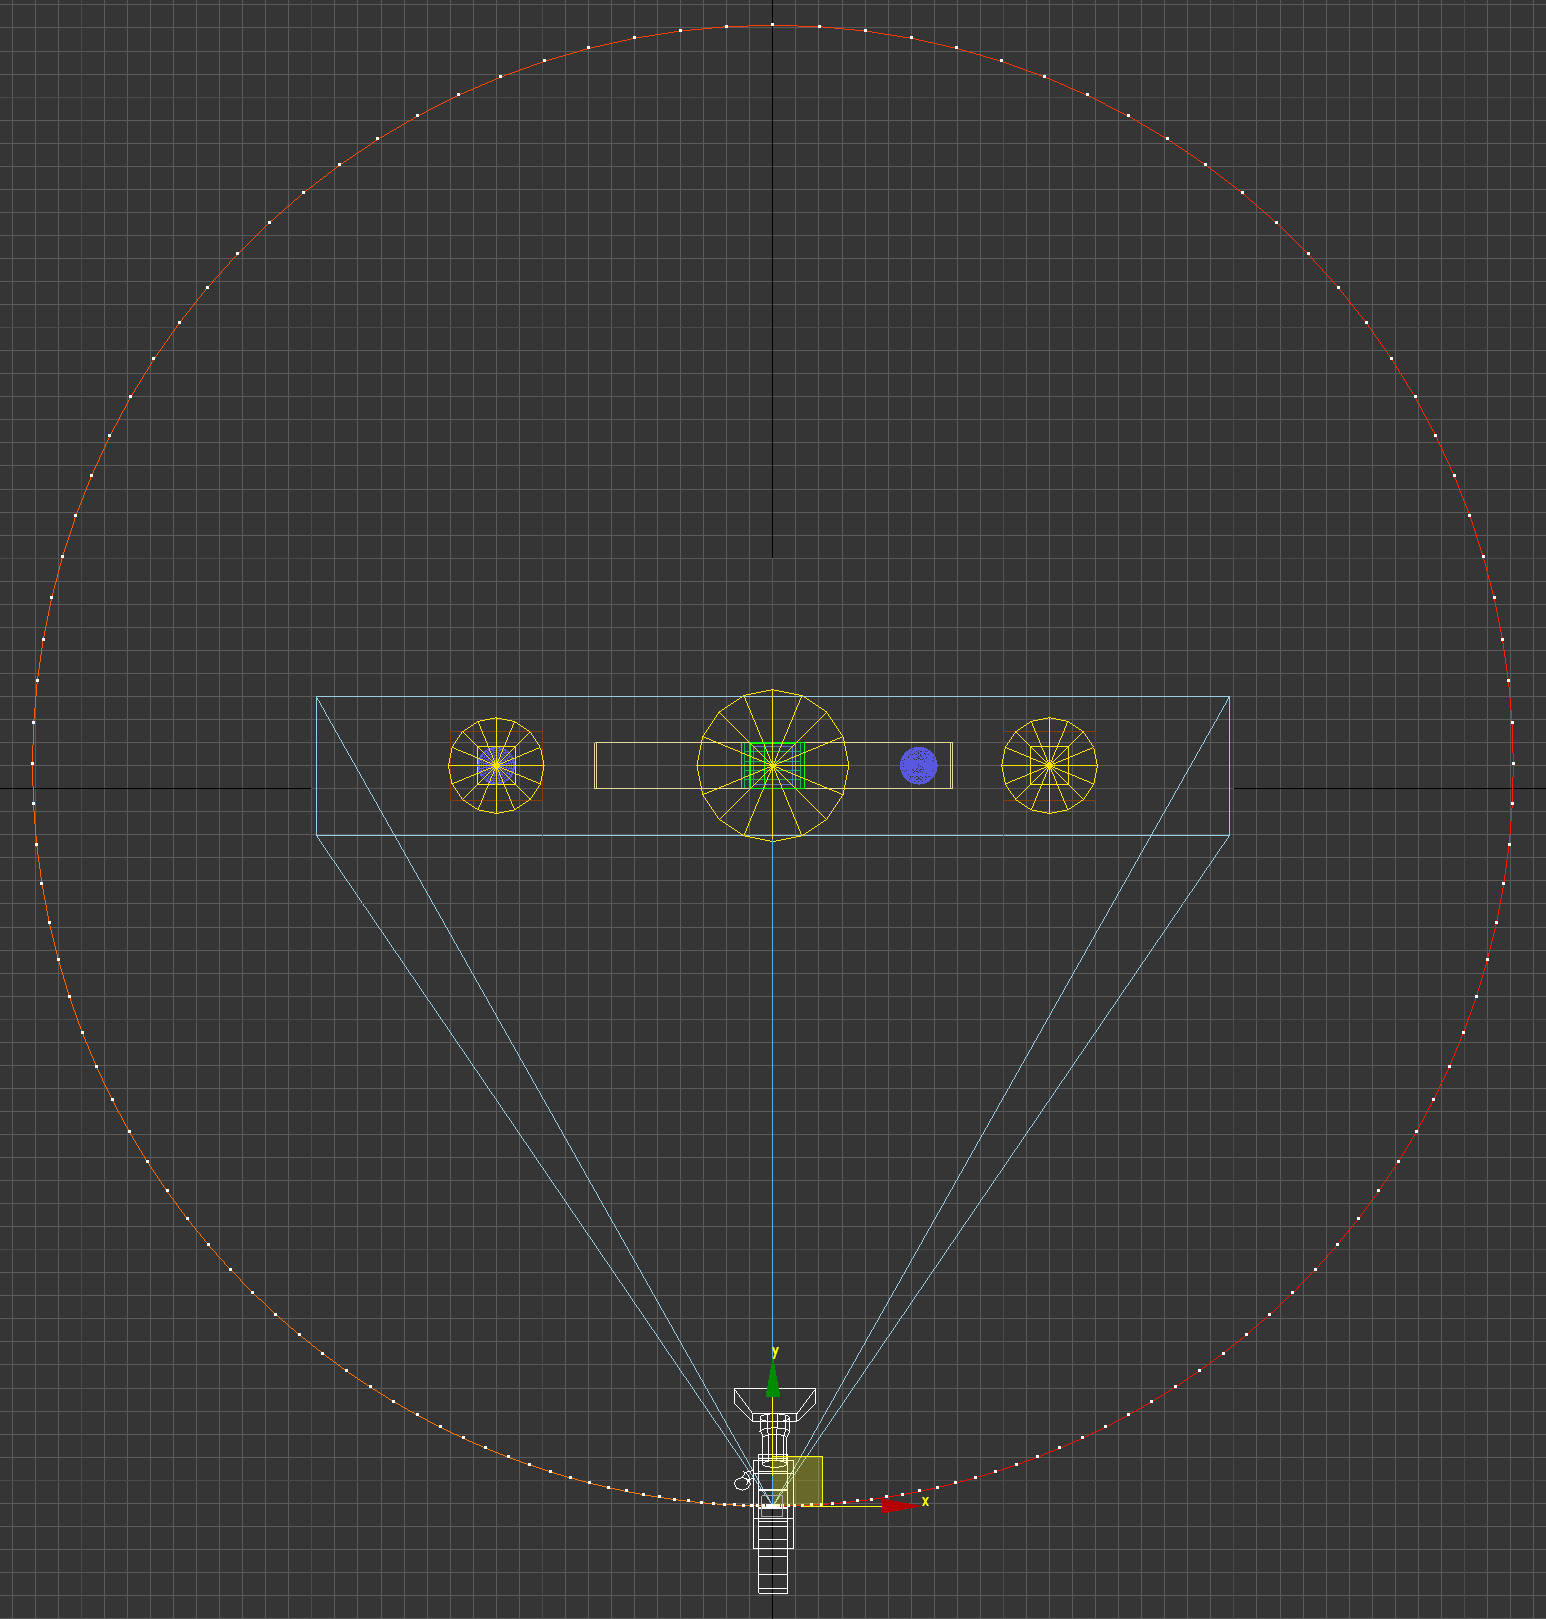
\includegraphics[width=0.5\textwidth]{imagenes/misc/CameraPath.png}
   \caption{Trayectoria final seguida por la cámara.}
\end{figure}

\bigskip

Y la posición del \textit{Dummy} y la cámara para que funcione correctamente es:

\begin{figure}[H]
   \centering
   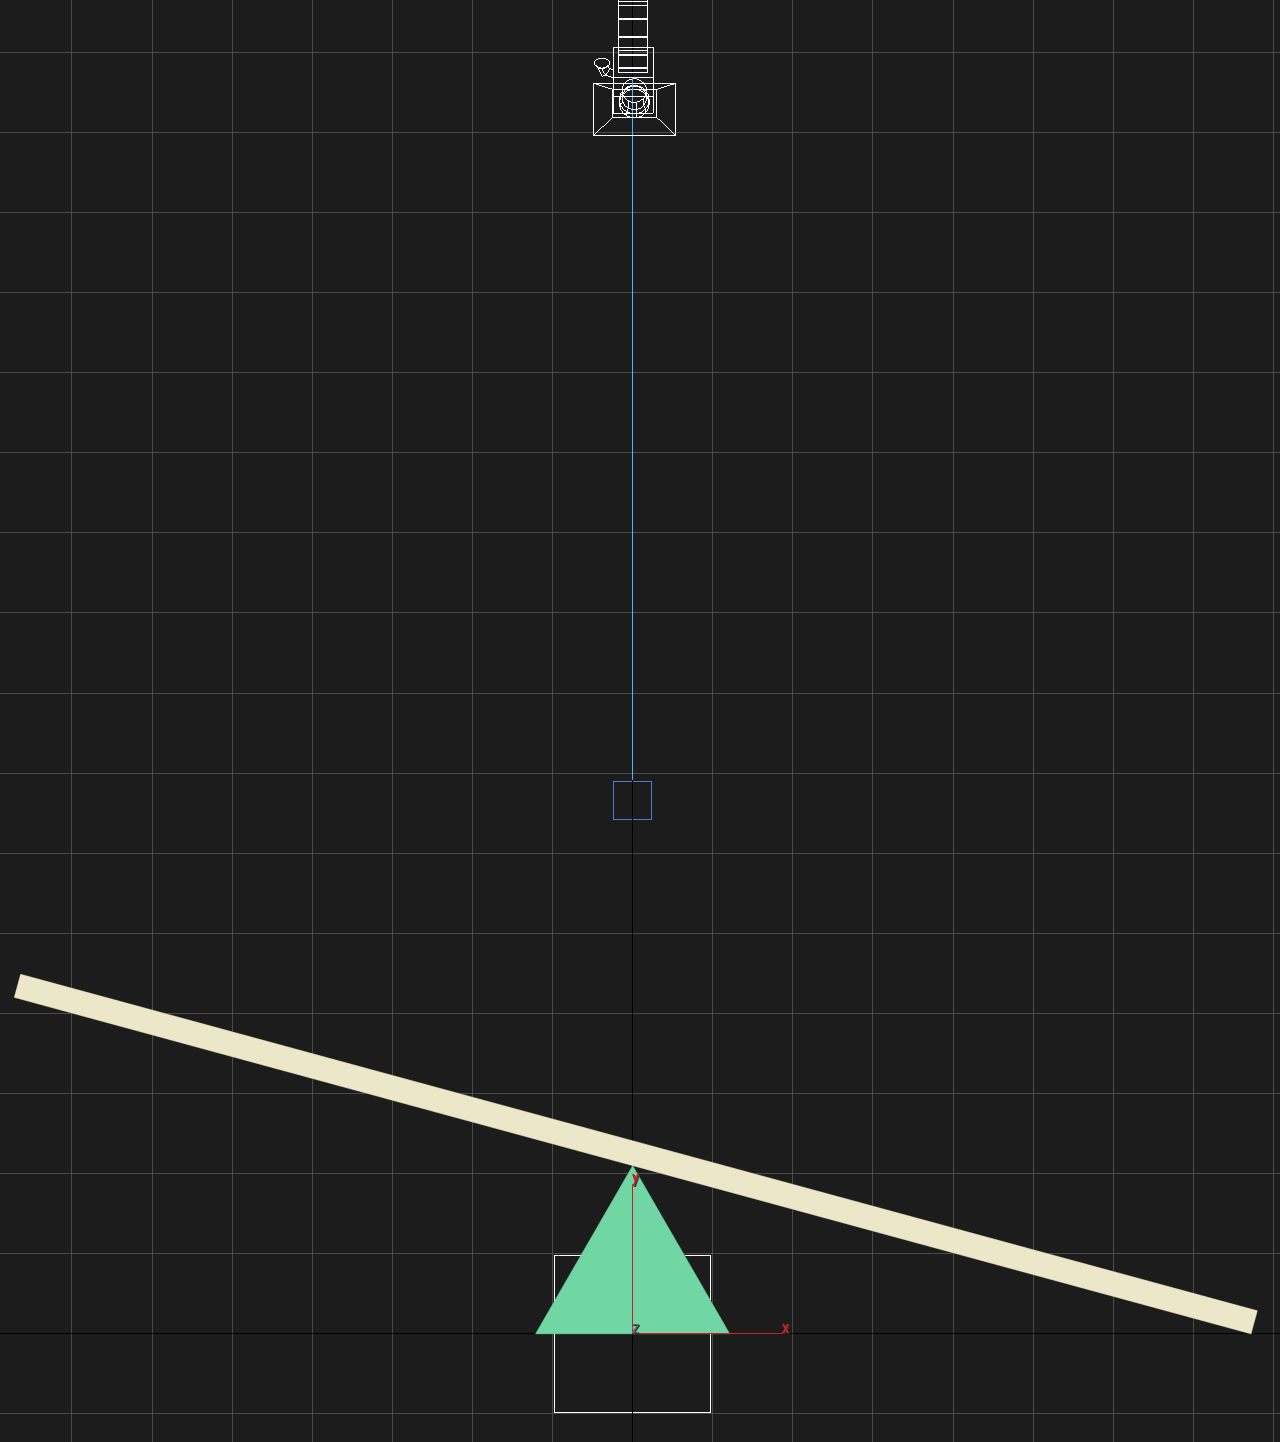
\includegraphics[width=0.5\textwidth]{imagenes/misc/DummyCamera.png}
   \caption{Cámara junto a su \textit{Dummy} en la escena. Así se consigue que la cámara apunte siempre a los objetos.}
\end{figure}

\newpage

\section{Configuración final}

Los instantes más importantes de la animación final, quitando el movimiento de la cámara para más claridad, son:

\begin{figure}[H]
    \centering 
\begin{subfigure}[t]{0.48\textwidth}
    \centering
    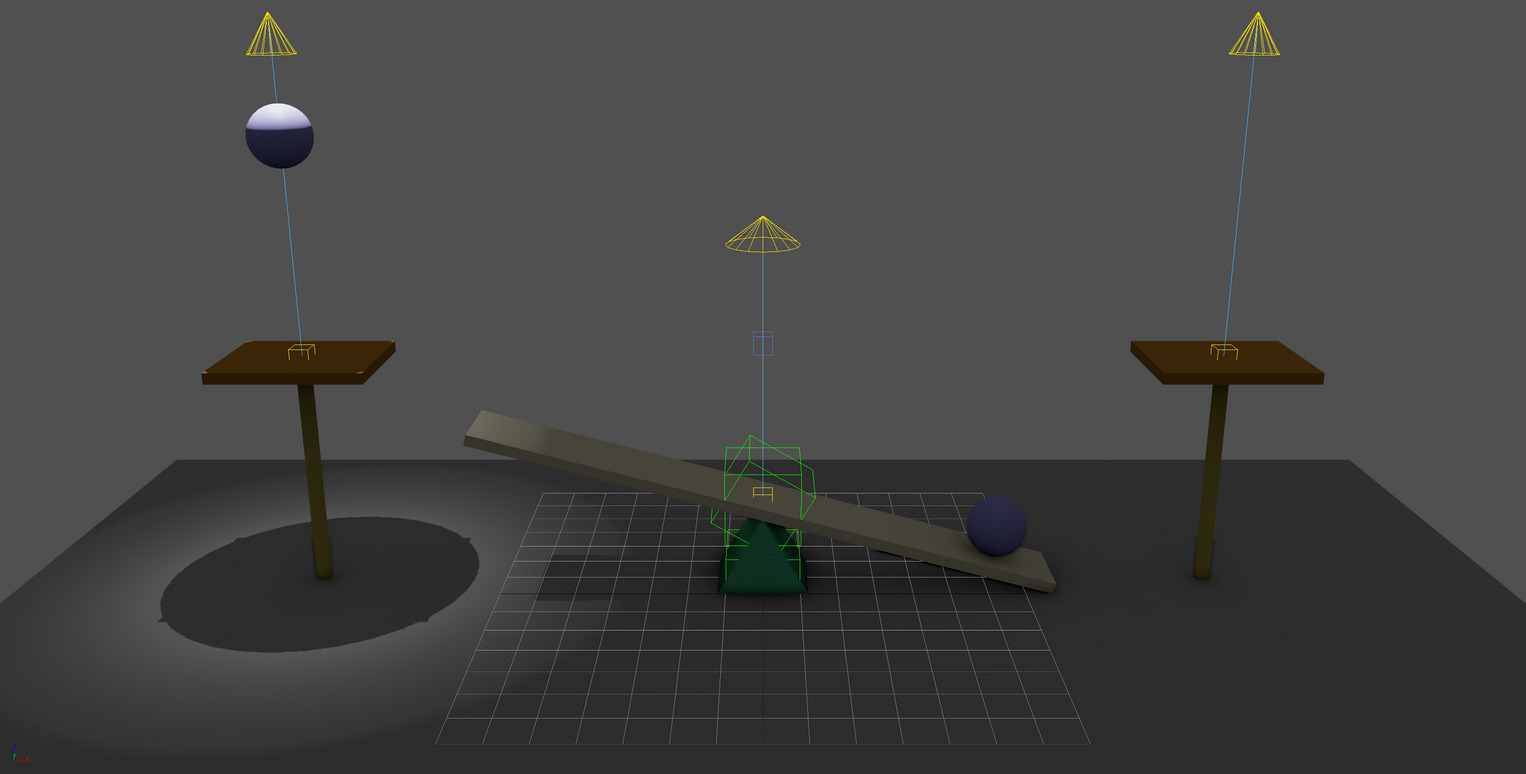
\includegraphics[width=\textwidth]{imagenes/animaciones/general/0.jpg}
    \caption{Animación de la escena en el instante 0.}
 \end{subfigure}
\hfill
 \begin{subfigure}[t]{0.48\textwidth}
    \centering
    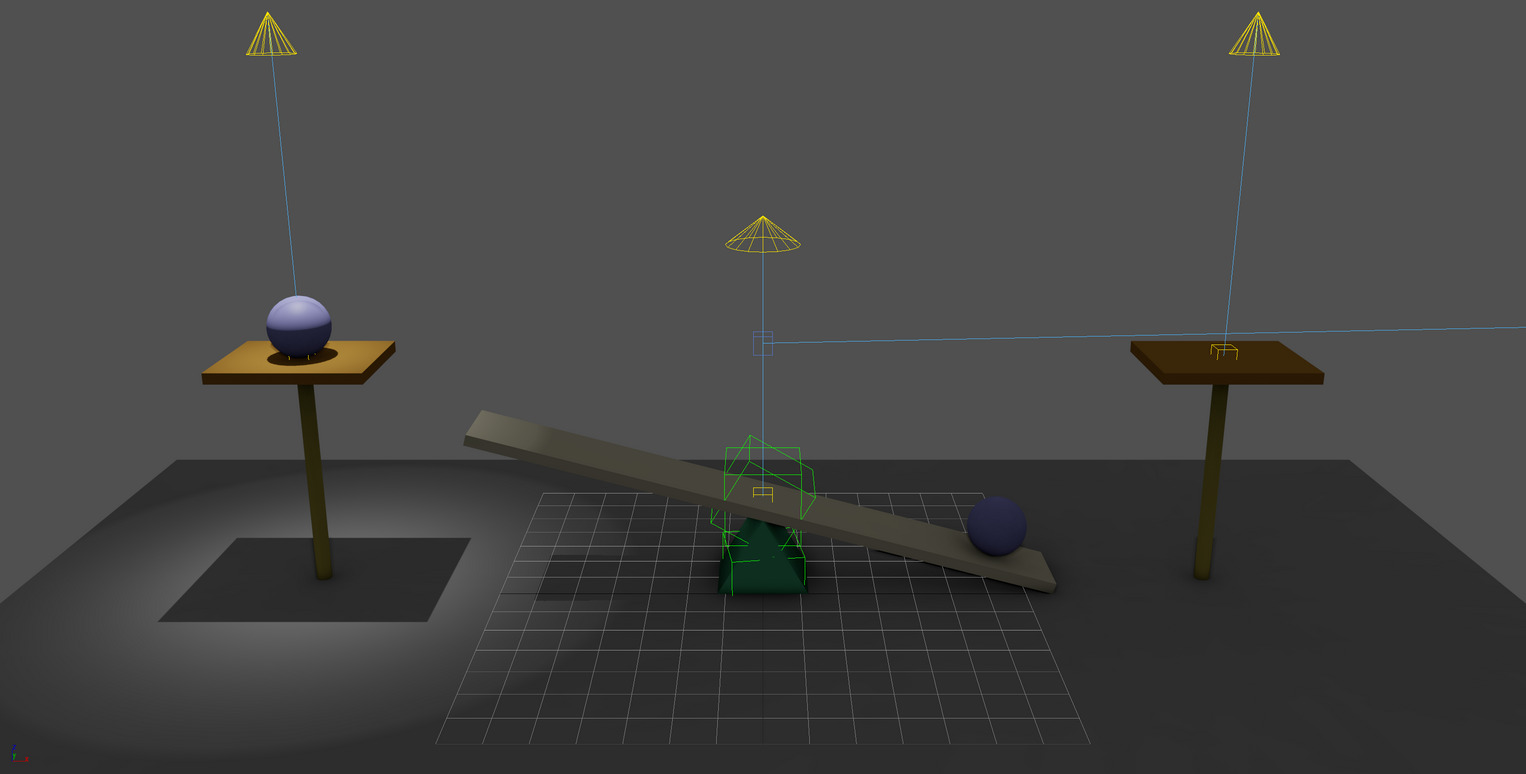
\includegraphics[width=\textwidth]{imagenes/animaciones/general/14.jpg}
    \caption{Animación de la escena en el instante 14.}
 \end{subfigure}
\hfill
 \begin{subfigure}[t]{0.48\textwidth}
    \centering
    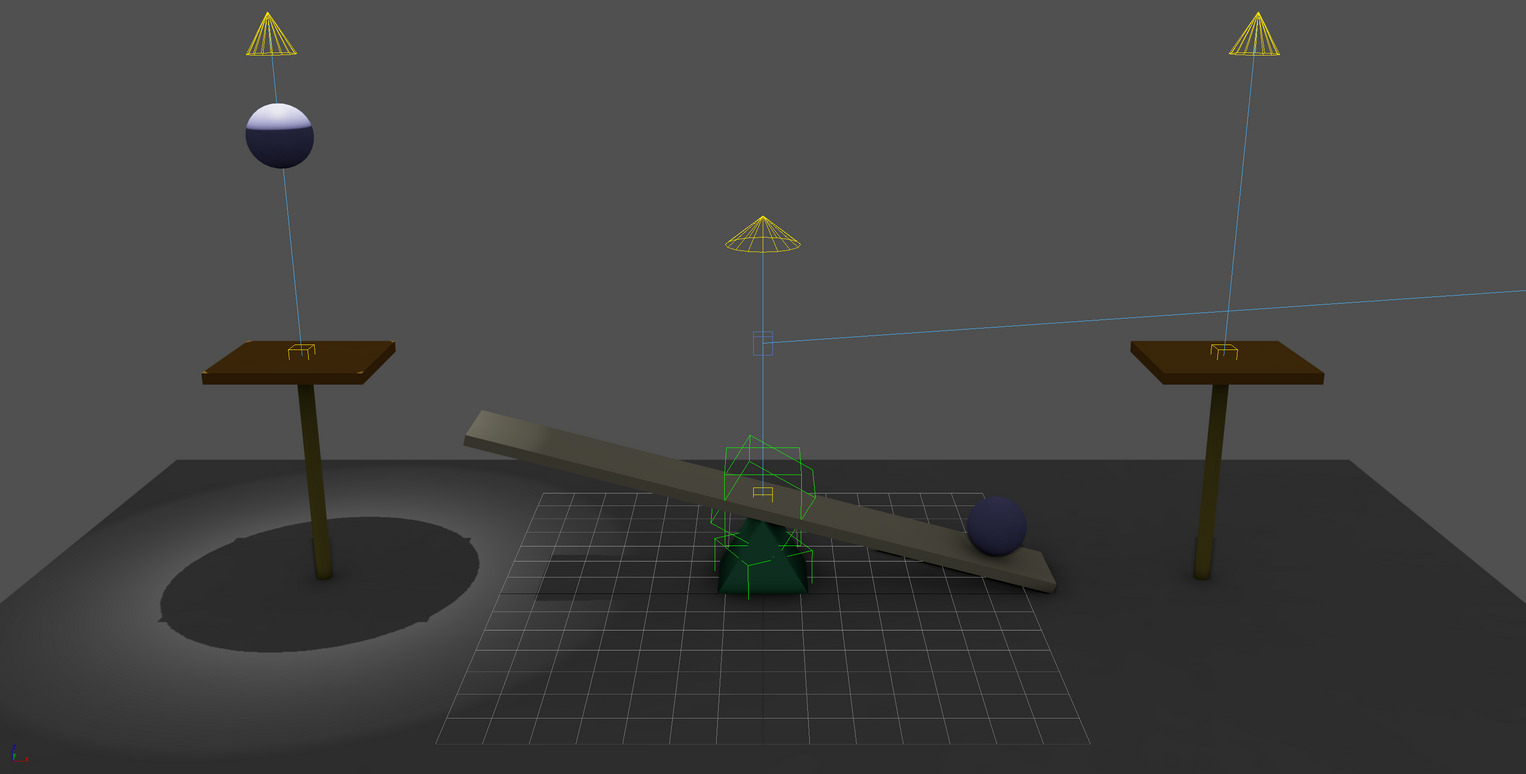
\includegraphics[width=\textwidth]{imagenes/animaciones/general/26.jpg}
    \caption{Animación de la escena en el instante 26.}
 \end{subfigure}
\hfill
 \begin{subfigure}[t]{0.48\textwidth}
    \centering
    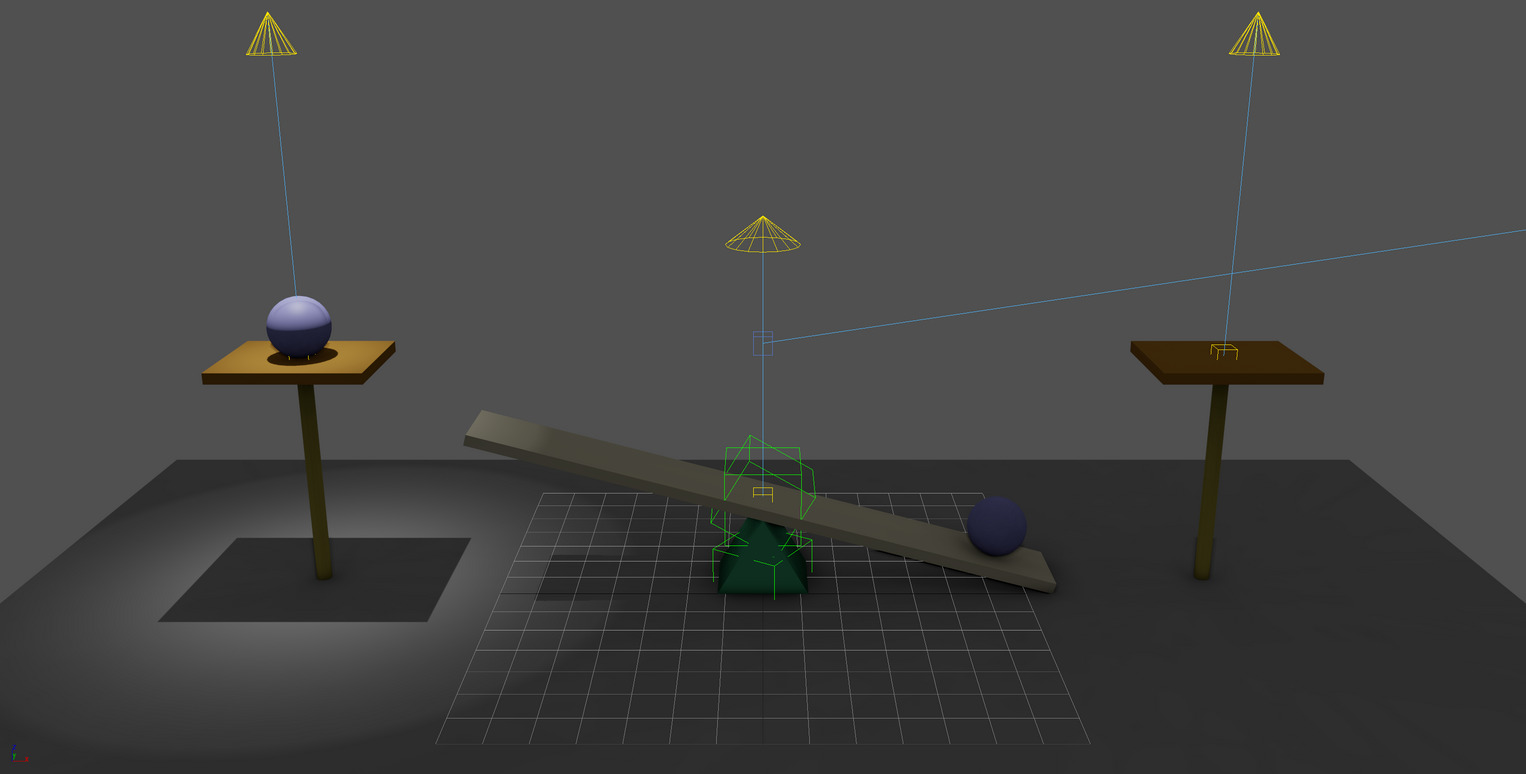
\includegraphics[width=\textwidth]{imagenes/animaciones/general/38.jpg}
    \caption{Animación de la escena en el instante 38.}
 \end{subfigure}
\hfill
 \begin{subfigure}[t]{0.48\textwidth}
    \centering
    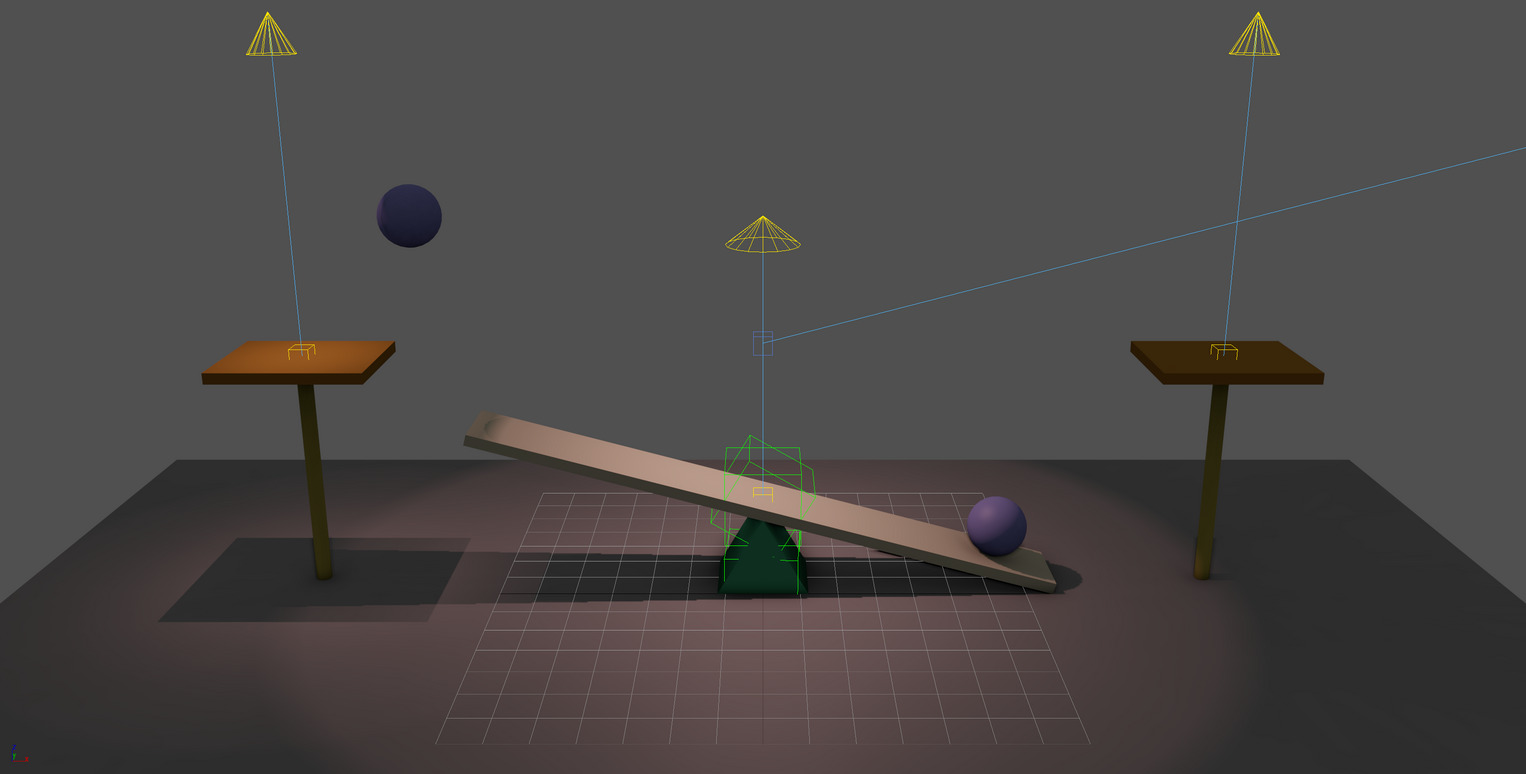
\includegraphics[width=\textwidth]{imagenes/animaciones/general/48.jpg}
    \caption{Animación de la escena en el instante 48.}
 \end{subfigure}
\hfill
 \begin{subfigure}[t]{0.48\textwidth}
    \centering
    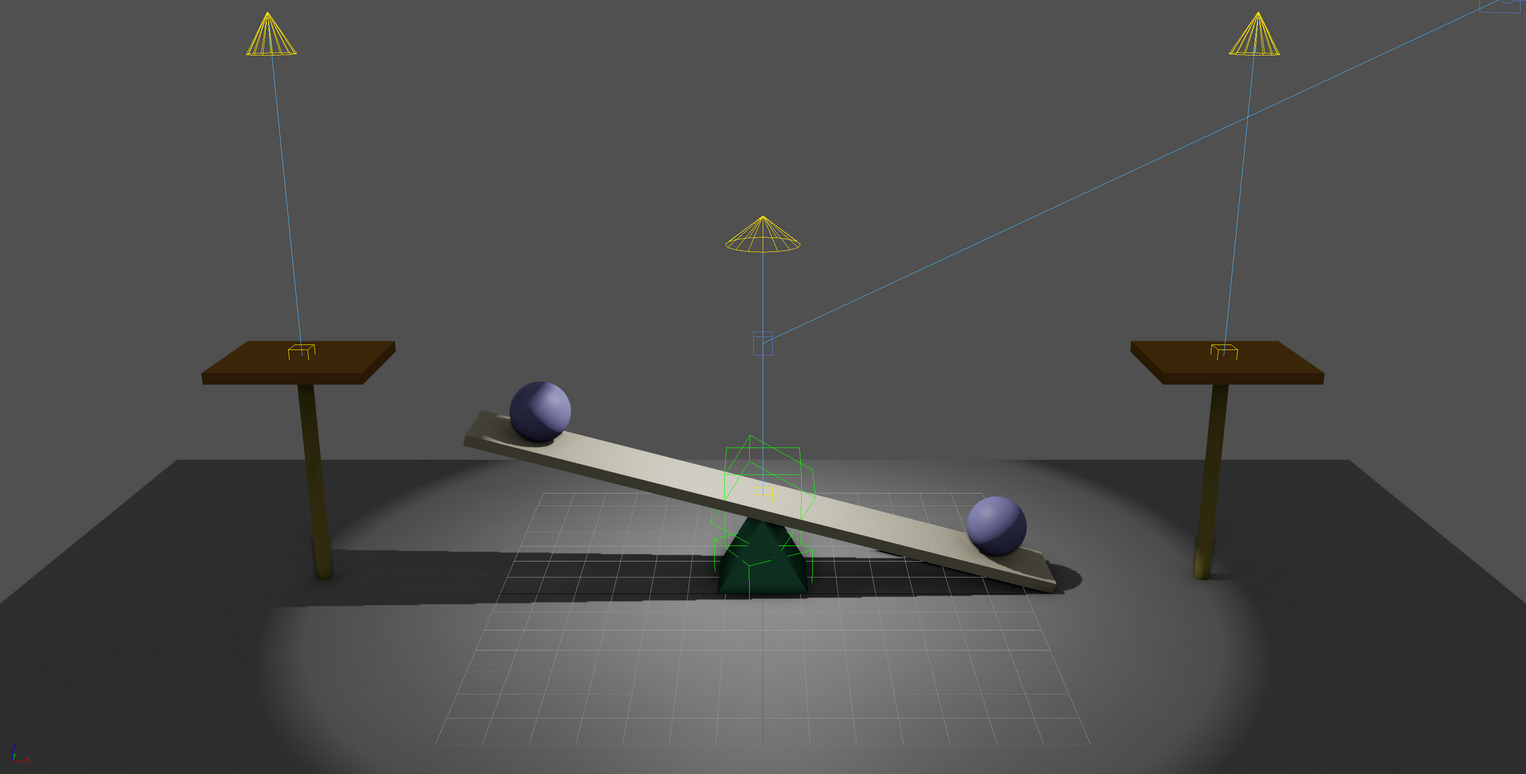
\includegraphics[width=\textwidth]{imagenes/animaciones/general/58.jpg}
    \caption{Animación de la escena en el instante 58.}
 \end{subfigure}
\hfill
 \begin{subfigure}[t]{0.48\textwidth}
    \centering
    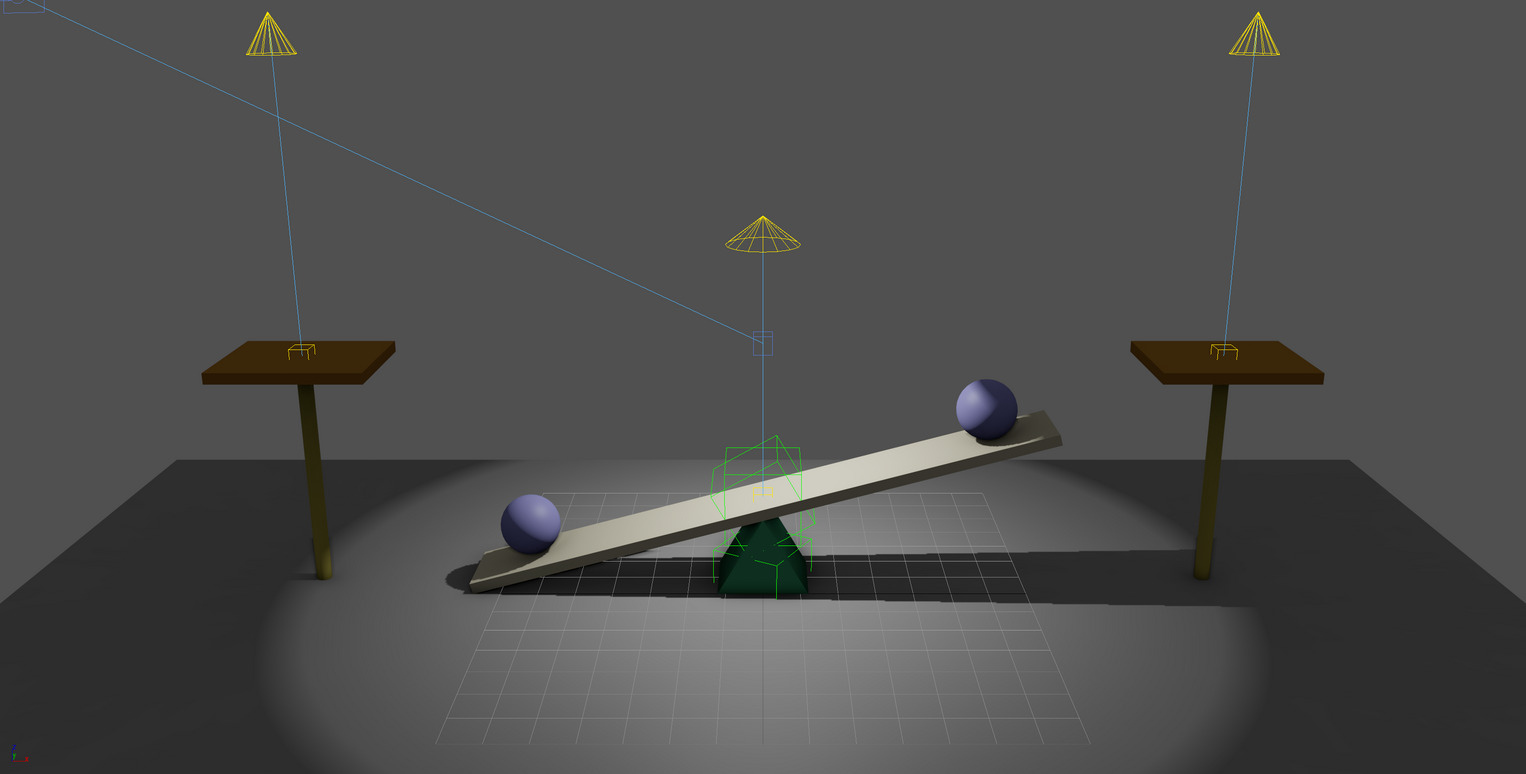
\includegraphics[width=\textwidth]{imagenes/animaciones/general/92.jpg}
    \caption{Animación de la escena en el instante 92.}
 \end{subfigure}
\hfill
 \begin{subfigure}[t]{0.48\textwidth}
    \centering
    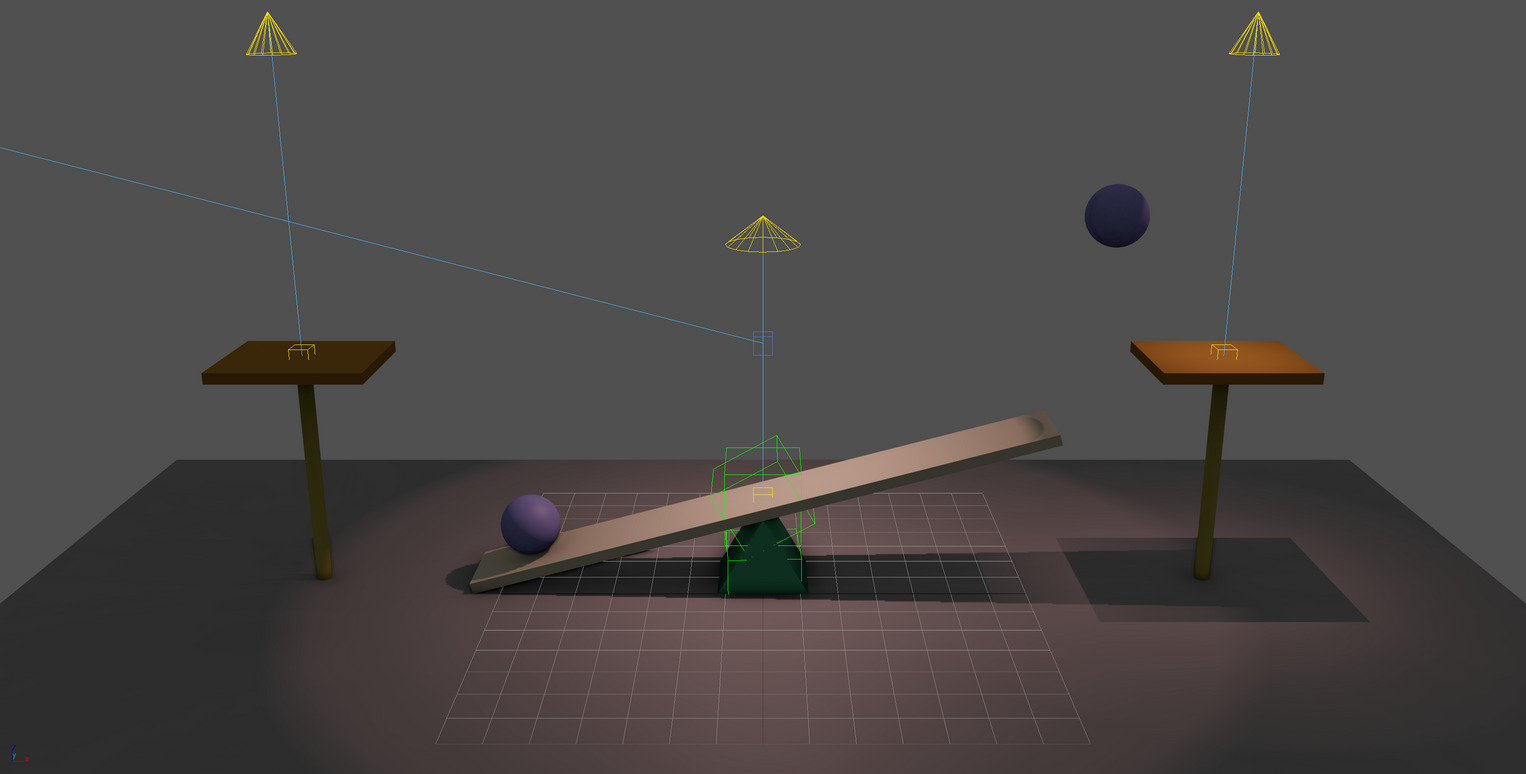
\includegraphics[width=\textwidth]{imagenes/animaciones/general/102.jpg}
    \caption{Animación de la escena en el instante 102.}
 \end{subfigure}
\hfill
 \begin{subfigure}[t]{0.48\textwidth}
    \centering
    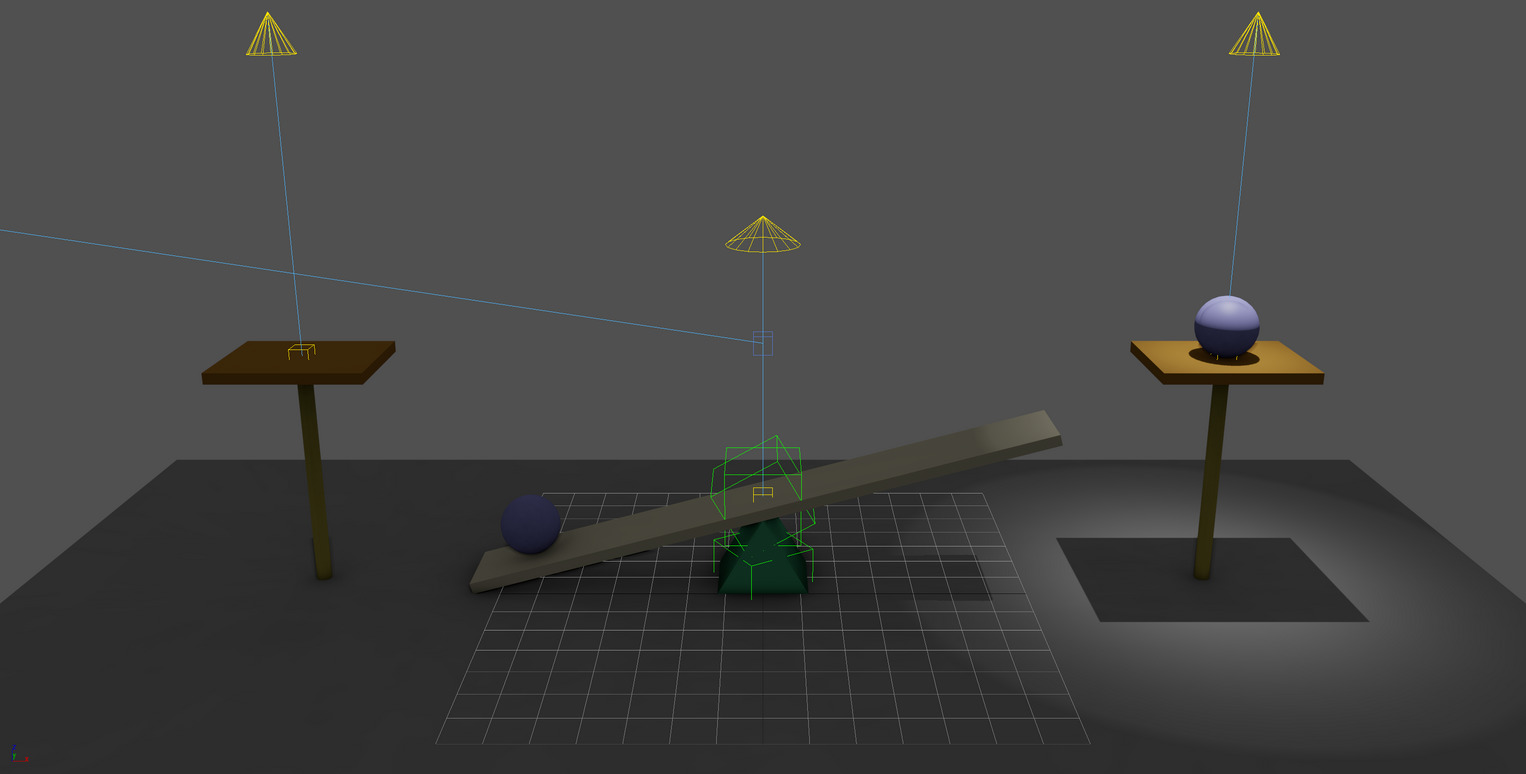
\includegraphics[width=\textwidth]{imagenes/animaciones/general/112.jpg}
    \caption{Animación de la escena en el instante 112.}
 \end{subfigure}
\hfill
 \begin{subfigure}[t]{0.48\textwidth}
    \centering
    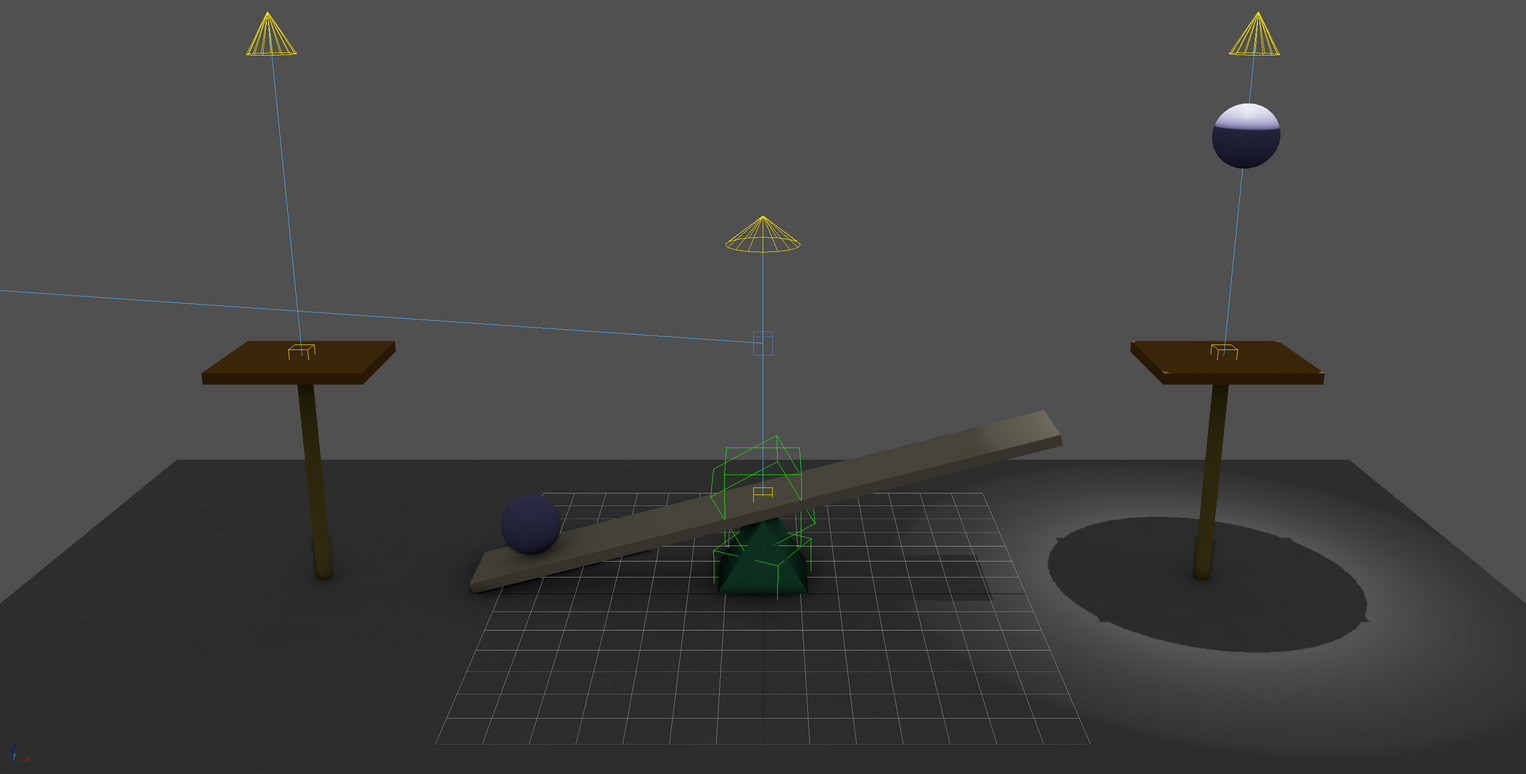
\includegraphics[width=\textwidth]{imagenes/animaciones/general/124.jpg}
    \caption{Animación de la escena en el instante 124.}
 \end{subfigure}
\end{figure}

\begin{figure}[H]\ContinuedFloat
 \begin{subfigure}[t]{0.48\textwidth}
    \centering
    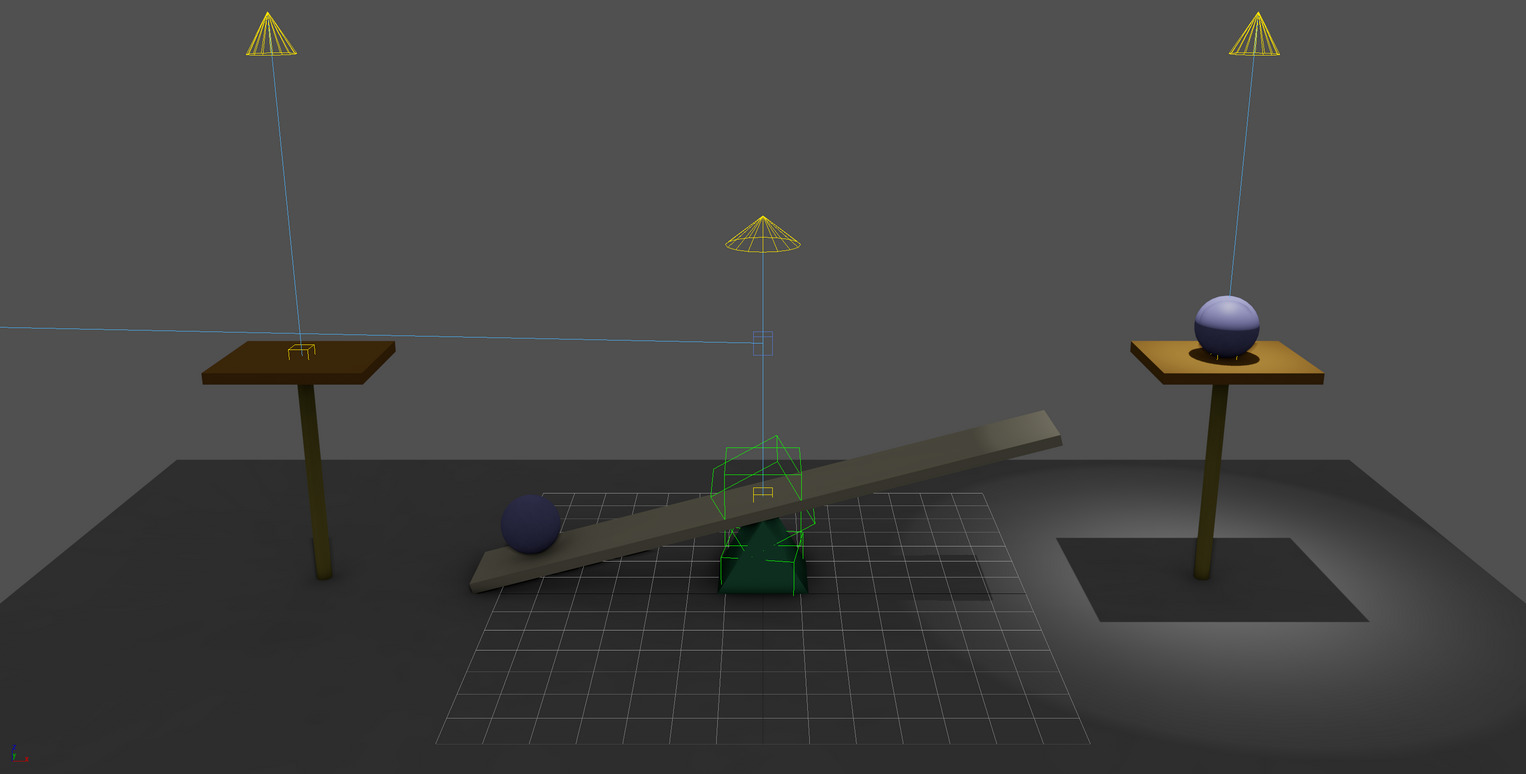
\includegraphics[width=\textwidth]{imagenes/animaciones/general/136.jpg}
    \caption{Animación de la escena en el instante 136.}
 \end{subfigure}
\hfill
 \begin{subfigure}[t]{0.48\textwidth}
    \centering
    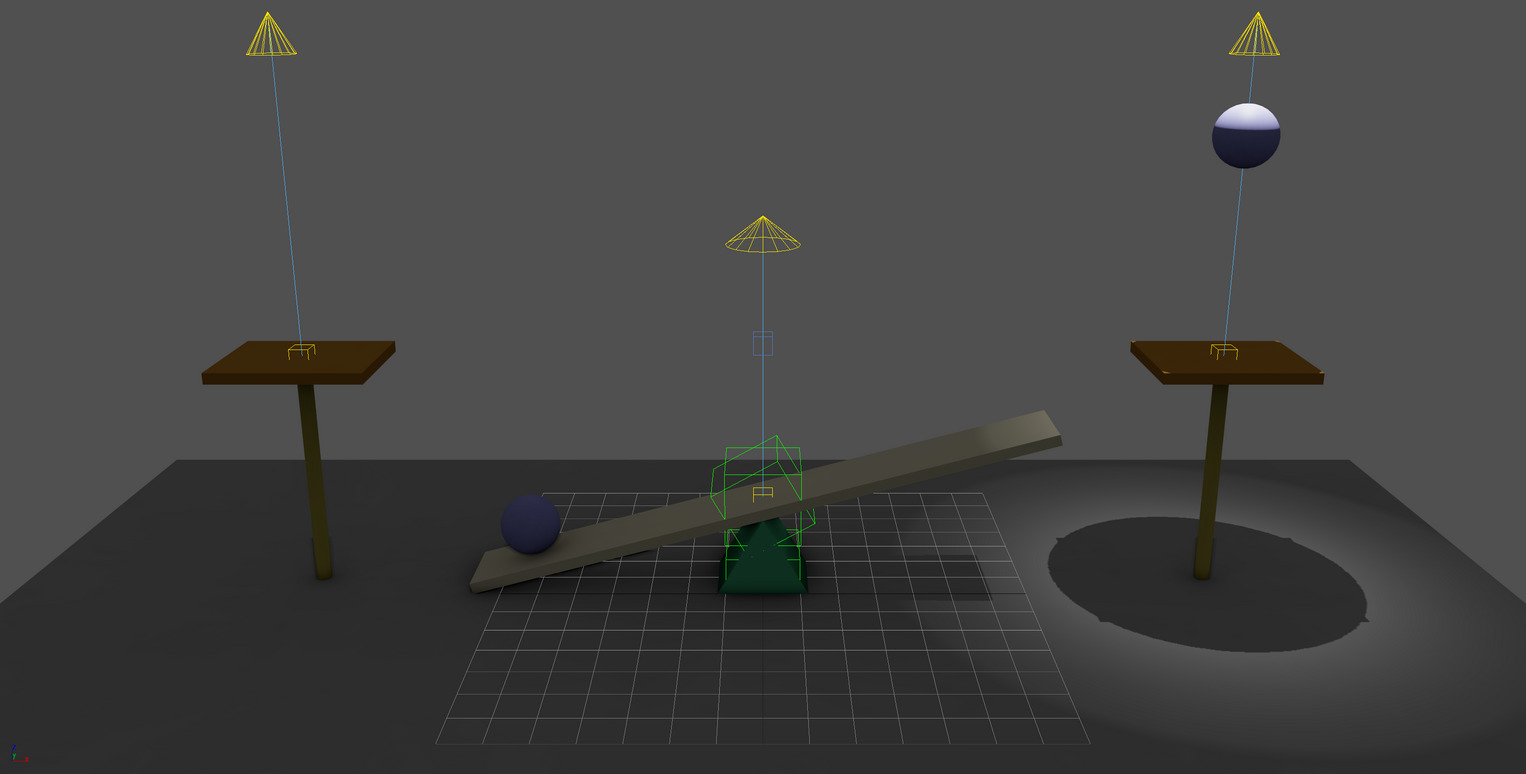
\includegraphics[width=\textwidth]{imagenes/animaciones/general/150.jpg}
    \caption{Animación de la escena en el instante 150.}
 \end{subfigure}
 \caption{Instantes más importantes de la animación resultante.}
\end{figure}
\end{document}
